\documentclass[a4paper,	11pt]{report}
% \usepackage[letterpaper,top=2cm,bottom=2cm,left=4cm,right=4cm,marginparwidth=1.75cm]{geometry}
% Include preambles
% ---------------- Packages ----------------
%\usepackage{hyphenat}

\usepackage[utf8]{inputenc}
\usepackage{graphicx}
% \usepackage[fleqn]{amsmath}
\usepackage{amsmath}
\usepackage{listings}
\usepackage[hidelinks]{hyperref}
% \usepackage{dtsyntax}
% \usepackage[colorinlistoftodos,prependcaption,textsize=tiny]{todonotes}
\usepackage[normalem]{ulem}
\usepackage{pdflscape}
\usepackage{amssymb}
\usepackage{longtable}
%\usepackage{tikz}
%\usepackage{algorithm}
\usepackage{tikz}
\usetikzlibrary{decorations.pathmorphing, calc, arrows.meta}

\usepackage{placeins}

\usepackage[a4paper,top=2.5cm,bottom=3cm,inner=2.5cm,outer=2.5cm]{geometry}
% \usepackage[letterpaper,top=2cm,bottom=2cm,left=4cm,right=4cm,marginparwidth=1.75cm]{geometry}

\usepackage{multirow}
% For \includegraphics with valign
\usepackage[export]{adjustbox}

\usepackage{tablefootnote}

% M: Tabla en vez de Cuadro
\usepackage[spanish,es-tabla]{babel}

\usepackage{xargs} % Use more than one optional parameter in a new commands

% Algorithms boxes
\usepackage{algorithm}
\usepackage{algorithmic}

% For \qtyrange and \hertz
\usepackage{siunitx}
\usepackage{textcomp}
\DeclareSIUnit{\pixel}{px}
\DeclareSIUnit{\fps}{fps}

\usepackage{subfig}
% \usepackage{subcaption}

% Code c++
\usepackage{listings}
\usepackage{xcolor}
\usepackage{tabularx}


\renewcommand{\lstlistingname}{Código}

% Define Modelica language style for listings
\lstdefinelanguage{Modelica}{
	keywords={
		algorithm, and, annotation, block, break, class, connect, connector,
		constant, discrete, each, else, elseif, elsewhen, encapsulated, end,
		enumeration, equation, expandable, extends, external, false, final,
		flow, for, function, if, import, in, initial, inner, input, loop,
		model, not, operator, or, outer, output, package, parameter, partial,
		protected, public, record, redeclare, replaceable, return, stream,
		then, true, type, when, while, within
	},
	sensitive=true,
	comment=[l]{//},
	morecomment=[s]{/*}{*/},
	morestring=[b]",
	morestring=[b]'
}

% Configure general listing settings
\lstset{
	language=Modelica,
	basicstyle=\small\ttfamily,
	keywordstyle=\color{blue}\bfseries,
	commentstyle=\color{gray}\itshape,
	stringstyle=\color{teal},
	numbers=left,
	numberstyle=\tiny\color{gray},
	stepnumber=1,
	numbersep=8pt,
	showstringspaces=false,
	breaklines=true,
	frame=single,
	captionpos=b
}


% ---------------- Macros / Custom commands ----------------

% Title page
\newcommand*{\titleGP}{\begingroup
    \centering
    \vspace*{\baselineskip}
    \thispagestyle{empty}

    \rule{\textwidth}{1.6pt}\vspace*{-\baselineskip}\vspace*{2pt}
    \rule{\textwidth}{0.4pt}\\[\baselineskip]

    {\LARGE Simulador en tiempo real de dinámica vehicular usando modelos orientados
a objetos. } \\[0.2\baselineskip]

    \rule{\textwidth}{0.4pt}\vspace*{-\baselineskip}\vspace{3.2pt}
    \rule{\textwidth}{1.6pt}\\[\baselineskip]

    \vspace*{2\baselineskip}

    
\includegraphics[width=0.3\textwidth]{img/logo-unr.png}

    \vspace*{2\baselineskip}

    \scshape
    Tesina de Grado\\[\baselineskip]
    Licenciatura en Ciencias de la Computación\par

    \vspace*{2\baselineskip}

    {\Large Autor: Juan Segundo Valero\\}
    {Legajo: V-3012/1}
    \vspace*{2\baselineskip}
    {\Large \\ Director: Ernesto Kofman} \vfill

    \vspace*{2\baselineskip}
    {\scshape \today} \\[0.3\baselineskip]

\endgroup}

\usepackage{amsmath}
\usepackage{amssymb}
\usepackage{amsopn}
\usepackage{mathtools}
\usepackage{float}

% set matrix maximum length
\setcounter{MaxMatrixCols}{20}

% math
\renewcommand{\vec}[1]{\boldsymbol{\mathbf{#1}}}
\newcommand{\norm}[1]{\lVert#1\rVert}

% Declare arg max and arg min functionss
\DeclareMathOperator*{\argmax}{arg\,max}
\DeclareMathOperator*{\argmin}{arg\,min}

% Declare atan2 
\DeclareMathOperator{\atantwo}{atan2}

% Homogeneous decoration function
\newcommand{\homo}[1]{\dot{#1}}


% Declare projection as math function
\DeclareMathOperator{\proj}{proj}
\newcommand{\fromCoord}[2]{{#1}_\mathrm{#2}}
\newcommand{\toCoord}[2]{\prescript{\mathrm{#2}}{}{#1}}
\newcommand{\worldCoordSystem}{\mathrm{W}}
\newcommand{\bodyCoordSystem}{\mathrm{B}}
\newcommand{\cameraCoordSystem}{\mathrm{C}}
\newcommand{\point}{\vec{p}}
\newcommand{\worldPoint}{\toCoord{\point}{\worldCoordSystem}}
\newcommand{\imagePoint}{\vec{u}}
\newcommand{\cameraPoint}{\toCoord{\point}{\cameraCoordSystem}}
\newcommand{\homoWorldPoint}{\toCoord{\homo{\point}}{\worldCoordSystem}}
\newcommand{\homoImagePoint}{\homo{\imagePoint}}
\newcommand{\homoCameraPoint}{\toCoord{\homo{\point}}{\cameraCoordSystem}}
\newcommand{\measurement}{\vec{z}}
\newcommand{\prediction}{\hat{\vec{z}}}
\newcommand{\seMatrix}{\vec{\xi}}
\newcommand{\transform}[2]{\toCoord{\fromCoord{\seMatrix}{#2}}{#1}}
\newcommand{\pointCoord}[1]{\toCoord{\point}{#1}}
\newcommand{\rotation}{\vec{R}}
\newcommand{\rotationCoord}[2]{\toCoord{\fromCoord{\rotation}{#2}}{#1}}
\newcommand{\translation}{\vec{t}}
\newcommand{\translationCoord}[2]{\toCoord{\fromCoord{\translation}{#2}}{#1}}
\newcommand{\intrinsicMatrix}{\vec{K}}
\newcommand{\principalPoint}{\vec{c}}
\newcommand{\reprojectionError}{u}
\newcommand{\projectionMatrix}{\vec{P}}
\newcommand{\cameraCenter}{\vec{o}}
\newcommand{\worldCameraCenter}{\toCoord{\cameraCenter}{\worldCoordSystem}}
\newcommand{\essentialMatrix}{\vec{E}}
\newcommand{\fundamentalMatrix}{\vec{F}}
\newcommand{\inverse}[1]{{#1}^{-1}}
\newcommand{\epipole}{\vec{e}}



% Localization (State Estiamtion)
\newcommand{\state}{x}
\newcommand{\observation}{z}
\newcommand{\controlCommand}{u}
\newcommand{\covariance}{\Sigma}
\newcommand{\motionModelNoise}{\epsilon}
\newcommand{\measurementModelNoise}{\delta}
\newcommand{\motionModelFunction}[1]{g\left( #1 \right)}
\newcommand{\observationModelFunction}[1]{h\left( #1 \right)}
\newcommand{\motionParametersCovariance}{R}
\newcommand{\observationModelCovariance}{Q}
\newcommand{\motionModelJacobian}{G}
\newcommand{\observationModelJacobian}{H}
\newcommand{\kalmanGain}{K}
\newcommand{\normalDistribution}[2]{\mathcal{N}\left( {#1}, {#2} \right)}
\newcommand{\motionModelJacobianControl}{V}
\newcommand{\motionModelCovariance}{M}
\newcommand{\stateEvolutionMatrix}{A}

% Mapping slides
\newcommand{\map}{m}
\newcommand{\mapRandomVariable}{m}

% SLAM slides
\newcommand{\informationMatrix}{\vec{\Omega}}
\newcommand{\error}{\vec{e}}
\newcommand{\observationBold}{\vec{z}}
\newcommand{\stateBold}{\vec{x}}
\newcommand{\jacobian}{\vec{J}}
\newcommand{\linearSystemb}{\vec{b}}
\newcommand{\linearSystemH}{\vec{H}}


% Motion Planning slides
\newcommand{\workSpace}{\mathcal{W}}
\newcommand{\obstaclesSet}{\mathcal{O}}
\newcommand{\robotInConfiguration}{\mathcal{A}}
\newcommand{\robotConfiguration}{q}
\newcommand{\configurationSpace}{\mathcal{C}}
\newcommand{\freeConfigurationSpace}{\configurationSpace_{free}}
\newcommand{\obstableConfigurationSpace}{\configurationSpace_{obs}}
\newcommand{\goalSet}{\configurationSpace_{goal}}
\newcommand{\startConfiguration}{\robotConfiguration_{I}}
\newcommand{\goalConfiguration}{\robotConfiguration_{G}}
\newcommand{\continuousPath}{\tau}
\newcommand{\motionLaw}{\gamma}
\newcommand{\robotActionSpace}{\mathcal{U}}


% Motion model
\newcommand{\position}{\vec{p}}
\newcommand{\orientation}{\vec{O}}
\newcommand{\orientationQuaternion}{\vec{q}}
\newcommand{\predictedPosition}{\hat{\vec{p}}}
\newcommand{\predictedOrientationQuaternion}{\hat{\vec{q}}}
\newcommand{\linearVelocity}{\vec{v}}
\newcommand{\angularVelocity}{\vec{\omega}}

\DeclareMathOperator{\slerpOp}{slerp}
\newcommand{\slerp}[1]{\slerpOp{\left( #1 \right)}}

% Map structure
\newcommand{\keyframesSet}{K}
\newcommand{\mapPointsSet}{P}
\newcommand{\observedMapPoints}{O}
\newcommand{\covisibilityKeyframes}{CK}
\newcommand{\localMap}{local\_map}

% Bundle Adjutment
\newcommand{\update}{\vec{\delta}}
\newcommand{\incremental}{\hat{\update}}


% Loop Closure names

% scaled operators and letters to fancy view
\newcommand{\sminus}{\scalebox{0.5}[1.0]{$-$}}
\newcommand{\splus}{\scalebox{0.6}[0.6]{$+$}}
\newcommand{\curr}{c}
\newcommand{\sind}[1]{\scalebox{0.6}[0.6]{$#1$}}
\newcommand{\ind}[1]{\scalebox{0.7}[0.7]{$#1$}}

\newcommand{\keyframe}{\vec{K}}
\newcommand{\bowVector}{\vec{v}}
\newcommand{\lcError}{\vec{\Omega}}
\newcommand{\relativeTransformation}{\seMatrix}
\DeclareMathOperator{\interpolate}{interpolate}

\newcommand{\relativeMotion}{\vec{\delta}}
\newcommand{\groundTruth}[1]{{#1}^{*}}

% definición del operador rot()
\DeclareMathOperator{\rotationOp}{rot}
\newcommand{\getRotation}[1]{\rotationOp{\left( #1 \right)}}

\DeclareMathOperator{\translationOp}{trans}
\newcommand{\getTranslation}[1]{\translationOp{\left( #1 \right)}}








% Document settings
% ---------------- Document settings and layout adjustments ----------------

% Page layout settings
\renewcommand\floatpagefraction{.9}
\renewcommand\topfraction{.9}
\renewcommand\bottomfraction{.9}
\renewcommand\textfraction{.1}
\setcounter{totalnumber}{50}
\setcounter{topnumber}{50}
\setcounter{bottomnumber}{50}



\begin{document}


% Title Page
\titleGP
\newpage
\thispagestyle{empty}

% Table of Contents
\tableofcontents

% 1 - Introducción

%   1.1 Motivación

%   1.2 Objetivos

%   1.3 Organización de la Tesina

% 2 - Herramientas y Antecedentes

%    2.1 Lenguaje Modelica

%    2.2 Librería Multicuerpos

%    2.3 Visualizadores

%   2.4 Simulaciones Man-in-the-Loop

%    2.5 Trabajos Relacionados

% 3 -  Desarrollo

%    3.1 Librería de Dinámica de Autos

%    3.2 Interfaces de Comunicación

%    3.3 Visualizador

% 4 - Ejemplos y Resultados

%   4.1 Modelos y Simulaciones a lazo abierto

%   4.2 Modelos y Simulaciones en tiempo real.

% 5 - Conclusiones

% 6 - Referencias Bibliográficas

% Abstract
\chapter*{Resumen}
\label{sec:abstract}
El prototipado digital y la simulación computacional se han consolidado como herramientas fundamentales en la industria automotriz y el automovilismo deportivo, permitiendo evaluar diseños en etapas tempranas y entrenar pilotos en entornos interactivos seguros (Driver-in-the-Loop). Sin embargo, el sector se encuentra dominado por plataformas comerciales cerradas, lo que evidencia una carencia de alternativas de código abierto basadas en técnicas de modelado modernas. Para abordar esta problemática, el presente trabajo propone el desarrollo de un simulador de dinámica vehicular interactivo, estrictamente modular y capaz de ejecutarse en tiempo real. El sistema propuesto se articula en tres componentes interoperables: un núcleo físico-matemático desarrollado en Modelica, que aprovecha su paradigma de lenguaje orientado a objetos para modelar la cinemática del chasis y la suspensión, una biblioteca de comunicación de baja latencia en C++ para la integración con hardware de simulación mediante las API SDL y DirectInput, y un entorno de visualización 3D sincrónico implementado en Unity. El objetivo es lograr una arquitectura de software desacoplada que facilite el intercambio de subsistemas mecánicos, validando la estabilidad numérica y el rendimiento del lazo cerrado conductor-simulador. De este modo, se busca sentar las bases y documentar una herramienta extensible que permita el acceso a la simulación vehicular de alta fidelidad para la investigación y el desarrollo independiente.

\chapter*{Agradecimientos}
\label{sec:acknowledgment}
Quiero agradecer a mi familia, por apoyarme todos estos años y darme todo lo que necesité y más para crecer como persona. \\

A mi director, Ernesto, por el gran acompañamiento que me dio en estos meses que hizo posible el desarrollo de esta tesina. \\

A todos los profesores de la carrera por darme una base excelente para formarme como científico de la computación. \\

A mis amigos, por ser siempre el apoyo que me ayudó a seguir adelante cuando necesitaba un empujón. \\
\vspace{1cm}

\begin{center}
	\textit{What would life be like if we only did what is necessary?} - Niki Lauda
\end{center}



% Preliminaries
\chapter{Introducción}
\label{sec:introduction}
\input{src/introduction.tex}

\section{Motivación}
\label{sec:motivation}
En la industria automotriz y el automovilismo deportivo modernos, el prototipado digital de vehículos ha adquirido una importancia fundamental. El constante aumento en los costos de desarrollo y fabricación, sumado a la creciente complejidad de los sistemas vehiculares, exige soluciones eficientes. Por ello, la industria está migrando aceleradamente hacia el uso de simulaciones avanzadas. Estas herramientas permiten evaluar diferentes enfoques de diseño en las etapas tempranas de construcción, lo que reduce drásticamente los costos, facilita la detección prematura de errores y permite analizar con precisión cómo se comporta dinámicamente el sistema en su conjunto.\\

Además de su valor en el diseño, este tipo de simulaciones se utiliza extensamente como herramienta de entrenamiento y preparación para pilotos de carreras (\textit{Driver-in-the-Loop}). Estos sistemas les permiten utilizar un entorno virtual que replica fielmente las condiciones reales de pista, a una fracción del costo y eliminando los riesgos físicos y materiales que implicaría realizar pruebas en un circuito.\\

Aunque existen plataformas comerciales robustas para llevar a cabo estas simulaciones, actualmente se observa una falta de alternativas de código abierto que integren las funcionalidades requeridas empleando técnicas y lenguajes de modelado modernos. Las soluciones en el mercado suelen ser propietarias y cerradas, lo que representa una barrera de entrada y limita severamente su adaptación, extensión o auditoría por parte de investigadores y desarrolladores independientes.\\

A esta limitación se suma la necesidad crítica de contar con una arquitectura de software inherentemente modular. El estudio de la dinámica vehicular exige una plataforma flexible, capaz de escalar en complejidad para satisfacer distintos objetivos de análisis o adaptarse a diferentes capacidades de cómputo. Para resolver este desafío, resulta coherente la adopción de Modelica. Gracias a su paradigma de modelado orientado a objetos, este lenguaje permite la encapsulación de cada componente físico, facilitando el intercambio fluido de los distintos subsistemas del vehículo y sentando las bases para una herramienta verdaderamente extensible e interoperable.\\


\section{Objetivo}
\label{sec:objective}
Como fue mencionado en la sección anterior, si bien existe software que permite realizar estas simulaciones, no hay actualmente herramientas libres basadas en el uso de lenguajes y técnicas modernas de modelado que integren las funcionalidades requeridas. \\

Con el objetivo de desarrollar un sistema que se acerque a cumplir estos requerimientos, se va a elaborar un proyecto en tres partes:
\begin{itemize}
    \item Una biblioteca en C++: Encargada de implementar una interfaz de comunicación de baja latencia con el hardware comercial utilizado en la simulación de vehículos (tales como servomotores para la respuesta del volante o Force Feedback, pedales y caja de cambios).
    \item Un modelo computacional en Modelica: Diseñado para simular la física y dinámica del vehículo. Este sistema procesará las entradas del conductor, calculará las fuerzas, momentos y transferencias de carga que afectan al vehículo, y emitirá los resultados de manera continua.
    \item Un entorno visualizador en Unity: Responsable de recibir la información de posicionamiento desde Modelica para renderizarla gráficamente, proporcionando al usuario una retroalimentación visual fluida.
\end{itemize}
Este sistema va a tener dos puntos de desarrollo claves: En primer lugar, la ejecución de la simulación en tiempo real estricto, lo cual es importante para que el modelo sea verdaderamente interactivo y útil para un conductor humano. En segundo lugar, su arquitectura modular. Al utilizar Modelica, un lenguaje de simulación orientado a objetos, resultará sencillo intercambiar diferentes partes y subsistemas del vehículo. Esto permitirá evaluar diversas geometrías de suspensión, modificar la rigidez de resortes y amortiguadores, o alterar componentes enteros con un esfuerzo mínimo. \\
Dada la complejidad de simular un vehículo completo, el desarrollo se concentrará principalmente en la simulación detallada del chasis y la cinemática de la suspensión. Sin embargo, la propia naturaleza de Modelica permitirá escalar el proyecto, dejando abierta la posibilidad de cambiar modelos simplificados (como los de neumáticos, motor o transmisión) por variantes más complejas si los requerimientos lo exigen. Finalmente, el diseño desacoplado asegura que las tres partes del sistema sean intercambiables; por ejemplo, se podría sustituir el visualizador en Unity por un software comercial alternativo, o adaptar la interfaz de los controles a hardware específico, sin comprometer la integridad del núcleo de simulación.

% \section{Trabajos publicados durante la tesina}
% \label{sec:publications}
% \input{src/publications.tex}

\section{Estructura del informe}
\label{sec:struture}
La siguiente tesina se organiza de la siguiente manera:

\begin{itemize}
    \item \textbf{Capítulo 2:} Desarrolla el marco teórico y el estado del arte. Aquí se introducen los conceptos matemáticos y computacionales fundamentales, así como las herramientas y antecedentes necesarios para comprender el proyecto.
    
    \item \textbf{Capítulo 3:} Detalla la implementación técnica del simulador. Se documenta el desarrollo del modelo físico-matemático de la dinámica vehicular, la construcción del entorno de visualización y la programación de la biblioteca de interfaces para la integración con el hardware.
    
    \item \textbf{Capítulo 4:} Presenta la validación del sistema y los resultados. Se exponen casos de estudio con el simulador en pleno funcionamiento, evaluando su rendimiento y estabilidad tanto en simulaciones precalculadas (lazo abierto) como en ejecuciones interactivas en tiempo real (lazo cerrado).
    
    \item \textbf{Capítulo 5:} Expone las conclusiones finales del trabajo. Se analizan los resultados obtenidos en contraste con los objetivos planteados, se discuten las limitaciones del modelo desarrollado y se proponen posibles líneas de trabajo futuro para la extensión y mejora de esta herramienta.
\end{itemize}

\chapter{Herramientas y Antecedentes}
\label{sec:prev_concepts}
\section{Simulación y modelado}
Antes de comenzar, se va a definir rápidamente los conceptos de simulación y modelado, ya que son la base de este proyecto. \\
El proceso de modelado se refiere a la extracción de conocimiento 
de un sistema físico que se desea simular, organizándolo de manera adecuada y representándolo de forma clara y sin ambigüedades. 
Por otro lado, el proceso de simulación hace referencia al desarrollo de experimentos sobre el modelo para hacer predicciones
sobre cómo se comportaría el sistema real si se fuesen a realizar los mismos experimentos sobre él  \cite{cellier2006}. \\


\section{Simulación de Sistemas Continuos}
Para el modelado del sistema físico, el siguiente proyecto adopta el paradigma de simulación de sistemas continuos. A diferencia de la simulación de eventos discretos, donde los cambios de estado ocurren de forma instantánea en momentos específicos, en un modelo continuo las variables del sistema evolucionan de manera ininterrumpida a lo largo del tiempo. Este comportamiento se define mediante sistemas de ecuaciones diferenciales ordinarias (ODE) y algebraicas diferenciales (DAE), las cuales describen las propiedades y la cinemática del modelo.\\


La elección de este enfoque es debido a la naturaleza dinámica de un vehículo. El comportamiento de un chasis involucra fenómenos físicos transitorios y de alta frecuencia, tales como la transferencia de carga, la compresión de los resortes de suspensión y el nivel de agarre variable. Es fundamental que el estado físico del vehículo esté definido para cualquier instante arbitrario $t$. Si no se garantizara esta continuidad matemática, se producirían vacíos de información o discontinuidades artificiales que alterarían las fuerzas resultantes, provocando inestabilidad numérica y un comportamiento dinámico completamente irreal. \\

\subsection{Modelos de ecuaciones diferenciales ordinarias (ODE)}

La forma más elemental de describir un sistema continuo es el modelo explícito de ecuaciones diferenciales ordinarias, también conocido como ODE o modelo en espacio de estados \cite{cellier2006}:
\begin{equation}
	\dot{\mathbf{x}}(t) = \mathbf{f}\bigl(\mathbf{x}(t), \mathbf{u}(t), t\bigr), \qquad \mathbf{x}(t_0) = \mathbf{x}_0
	\label{eq:state_space}
\end{equation}

$\mathbf{x}$ es el vector de estado,  $\mathbf{u}$ el vector de entradas y $t$ representa el tiempo. Las variables que se quieren observar como resultado de la simulación se obtienen mediante ecuaciones de salida que dependen únicamente de los estados y las entradas, $\mathbf{y} = \mathbf{g}(\mathbf{x}, \mathbf{u}, t)$. \\

Las variables de estado son las salidas de los integradores del modelo. No es el modelo quien las calcula, sino el algoritmo de integración numérica, el modelo solo debe proveer las derivadas de los estados  $\dot{\mathbf{x}}$. El modelo calcula $\dot{\mathbf{x}}(t_k)$ a partir de $\mathbf{x}(t_k)$, y el algoritmo de integración calcula $\mathbf{x}(t_{k+1})$ a partir de ambos \cite{cellier2006}.

Mientras $\mathbf{f}$ y sus derivadas no presenten discontinuidades, cada trayectoria de estado $x_i(t)$ es una función continua del tiempo, y puede aproximarse mediante un desarrollo en serie de Taylor alrededor de cualquier punto de la trayectoria:
\begin{equation}
	x_i(t^* + h) = x_i(t^*) + f_i(t^*)\cdot h + \frac{d f_i(t^*)}{dt}\cdot\frac{h^2}{2!} + \dots
\end{equation}
Los distintos algoritmos de integración difieren en cómo aproximan las derivadas de orden superior y en la cantidad de términos de la serie que consideran \cite{cellier2006}.

\subsection{Modelos de ecuaciones algebraico-diferenciales (DAE)}
\label{sec:dae_section}
Para muchos sistemas físicos no resulta sencillo ni natural formular el modelo como un sistema ODE. Lo habitual es obtener un conjunto de ecuaciones en el que las derivadas de los estados aparecen de forma implícita, mezcladas con ecuaciones algebraicas. A este tipo de descripciones se las denomina ecuaciones algebraico-diferenciales (DAE) y en su forma implícita más general se escriben como \cite{cellier2006}:

\begin{equation}
	\mathbf{f}\bigl(\mathbf{x}, \dot{\mathbf{x}}, \mathbf{u}, t\bigr) = \mathbf{0}
	\label{eq:implicit_dae}
\end{equation}

El modelado orientado a objetos de sistemas físicos conduce a descripciones DAE implícitas. Cada componente aporta sus propias ecuaciones constitutivas y las conexiones entre componentes agregan más ecuaciones de acoplamiento. El resultado es un sistema en el cual ninguna ecuación indica qué variable debe calcularse a partir de ella \cite{cellier2006}. En este estado las ecuaciones son acausales, es decir, el signo igual expresa una igualdad y no una asignación. \\

%El modelado orientado a objetos de sistemas físicos conduce invariablemente a descripciones DAE implícitas. Cada componente aporta sus propias ecuaciones constitutivas, y las conexiones entre componentes aportan ecuaciones adicionales de acoplamiento; el resultado es un sistema extenso en el que ninguna ecuación indica qué variable debe calcularse a partir de ella \cite{cellier2006}. En este estado las ecuaciones son \textit{acausales}: el signo igual expresa una igualdad y no una asignación. Esto refleja una propiedad de la física misma, en la que la causalidad computacional de una ley no está predeterminada. En una resistencia, por ejemplo, no puede afirmarse que la corriente provoque la caída de tensión ni que la diferencia de potencial provoque la corriente; ambas son aspectos simultáneos de un mismo fenómeno, y según el contexto el cálculo deberá adoptar una u otra dirección \cite{cellier2006}. \\


Un modelo DAE implícito puede convertirse en uno explícito decidiendo qué variable se despeja de cada ecuación (ordenamiento horizontal) y ordenando las ecuaciones de modo que ninguna variable se utilice antes de ser calculada (ordenamiento vertical). Después de aplicar este proceso, cada incógnita aparece exactamente una vez, a la izquierda del signo igual y estos pasan a funcionar como asignaciones. Si después se sustituyen las ecuaciones explícitas hasta que las derivadas de los estados dependan únicamente de los estados y las entradas, se obtiene el modelo ODE de la Ecuación (2.1) \cite{cellier2006}. Existen algoritmos que realizan este ordenamiento de forma automática, como las variantes del algoritmo de Tarjan \cite{cellier2006}. \\

Sin embargo, no todo sistema DAE puede ordenarse por completo. Pueden aparecer dos tipos de dificultades estructurales \cite{cellier2006}:

\begin{itemize}

	
	\item \textbf{Lazos algebraicos:} Subconjuntos de ecuaciones en los que cada ecuación y cada incógnita resultante dependen de al menos otras dos, por lo que no es posible despejarlas individualmente y deben resolverse al mismo tiempo, ya sea simbólicamente o mediante iteración numérica.
	
	\item \textbf{Singularidades estructurales:} Situaciones en las que existen restricciones algebraicas entre variables de estado, por lo que no son independientes entre sí y el sistema tiene menos grados de libertad que los integradores.
\end{itemize}

Estas dificultades se miden usando el índice de perturbación del sistema. Un DAE de índice $0$ no contiene lazos algebraicos ni singularidades estructurales, uno de índice $1$ tiene lazos algebraicos pero no singularidades y uno de índice mayor a $1$ (también conocido como DAE de índice superior) contiene singularidades estructurales  \cite{cellier2006}. Existen algoritmos de reducción de índice, como el de Pantelides que diferencian simbólicamente las ecuaciones de restricción para disminuir el índice del sistema en una unidad por aplicación del algoritmo. \\

Una vez formulado un modelo DAE, existen dos caminos para simularlo: convertirlo en un modelo ODE explícito que luego se integra con los métodos numéricos tradicionales o resolverlo directamente con un solver de DAE. En este último caso, al aplicar una fórmula de integración implícita a la ecuación (2.3), las derivadas $\dot{\mathbf{x}}_{k+1}$ se expresan en función de los estados, y el paso de integración se reduce a un sistema de ecuaciones no lineales $\mathbf{F}(\mathbf{x}_{k+1}) = \mathbf{0}$ \cite{cellier2006}. \\

%Una vez formulado un modelo DAE, existen dos caminos para simularlo: convertirlo simbólicamente en un modelo ODE explícito que luego se integra con los métodos numéricos tradicionales, o resolverlo directamente con un \textit{solver} de DAE. En este último caso, al aplicar una fórmula de integración implícita a la Ecuación~\eqref{eq:implicit_dae}, las derivadas $\dot{\mathbf{x}}_{k+1}$ se expresan en función de los estados, y el paso de integración se reduce a un sistema de ecuaciones no lineales $\mathbf{F}(\mathbf{x}_{k+1}) = \mathbf{0}$ que se resuelve por iteración de Newton \cite{cellier2006}. \\

Esto resulta relevante para los sistemas mecánicos multicuerpo. Formular un modelo ODE de un sistema de este estilo no es práctico, mientras que un modelo DAE es relativamente sencillo de obtener, alcanza con describir la dinámica de cada cuerpo por separado y agregar las interacciones entre ellos como ecuaciones de restricción. Este procedimiento suele dar lugar a modelos de índice $3$ con restricciones no lineales, en especial si hay topologías con bucles cinemáticos cerrados \cite{cellier2006}. Además, la cantidad de ecuaciones depende fuertemente de la elección de variables de estado, una elección descuidada puede hacer que crezca con la cuarta potencia de la cantidad de articulaciones, mientras que una elección adecuada logra que crezca solo linealmente \cite{cellier2006}.\\

%Esta distinción resulta particularmente relevante para los sistemas mecánicos multicuerpo. Formular un modelo ODE de un sistema multicuerpo complejo no es práctico, mientras que un modelo DAE es relativamente sencillo de obtener: basta con describir la dinámica de cada cuerpo por separado y agregar las interacciones entre ellos como ecuaciones de restricción. No obstante, este procedimiento suele dar lugar a modelos de índice~3 con restricciones fuertemente no lineales, en especial en topologías con lazos cinemáticos cerrados \cite{cellier2006}. Además, la cantidad de ecuaciones resultante depende fuertemente de la elección de las variables de estado: una elección descuidada puede hacer que crezca con la cuarta potencia de la cantidad de articulaciones, mientras que una elección adecuada logra que crezca solo linealmente. Por este motivo, la biblioteca multicuerpo desarrollada por Martin Otter no recurre al algoritmo de Pantelides, sino que formula sus ecuaciones de modo que las singularidades estructurales queden resueltas desde la propia formulación del modelo \cite{cellier2006}. \\

\subsection{Solvers}

Como se mencionó anteriormente, una vez traducido y compilado, el conjunto de componentes del sistema de simulación pasa a un sistema de ecuaciones algebraico-diferenciales (DAE). La integración de este sistema en el tiempo no puede realizarse de forma analítica, por lo que se recurre a métodos de integración numérica (\textit{solvers}). En el marco de OpenModelica se evaluaron dos solvers de referencia para la ejecución de la simulación: DASSL y CVODE. Ambos comparten la característica de ser especialmente adecuados para sistemas \textit{rígidos} (\textit{stiff}), condición que presenta el modelo del vehículo debido a la coexistencia de dinámicas de muy distinta escala temporal. A continuación se va a explicar el funcionamiento de ambos, lo cual va a resultar necesario para comprender esta tesina.

\subsubsection*{DASSL}

DASSL (\textit{Differential/Algebraic System Solver}) es el solver por defecto de OpenModelica, desarrollado por Petzold en Sandia National Laboratories \cite{petzold1982}. La principal ventaja es que opera directamente sobre la forma implícita  $F(t, y, \dot{y}) = 0$, más general que la forma explícita estándar $\dot{y} = f(t, y)$, lo que lo hace más apto ante sistema DAE como los que surgen del análisis dinámico de sistemas mecánicos multicuerpo. En particular, DASSL es aplicable incluso  cuando la matriz jacobiana $\partial F / \partial \dot{y}$ es singular, situación habitual en presencia de restricciones algebraicas.


El algoritmo se basa en la idea de Gear de reemplazar la derivada $\dot{y}$ en la ecuación implícita por una aproximación en diferencias, y resolver la ecuación no lineal resultante en el instante actual $t_n$ mediante el método de Newton. Para ello, emplea la fórmula de diferenciación regresiva (\textit{Backward Differentiation Formula}, BDF) de orden $k$, con $k$ variable entre $1$ y $5$. En su forma más simple, de primer orden, la aproximación es:

\begin{equation}
	F\!\left(t_n,\, y_n,\, \frac{y_n - y_{n-1}}{\Delta t_n}\right) = 0
\end{equation}

En cada paso, DASSL selecciona automáticamente tanto el orden $k$ como el tamaño de paso $\Delta t_n$ en función del comportamiento de la solución y de una estimación del error local de truncamiento, empleando además una formulación BDF de coeficiente líder fijo (\textit{fixed-leading-coefficient}) que mejora la estabilidad numérica. La ecuación no lineal se resuelve con una variante del método de Newton cuya matriz de iteración,

\begin{equation}
	G = \frac{\partial F}{\partial \dot{y}} + \alpha\, \frac{\partial F}{\partial y}
\end{equation}

donde $\alpha$ es un escalar que depende del paso y el orden. se factoriza y se reutiliza durante tantos pasos como sea posible para reducir el coste computacional. Su robustez frente a la forma DAE completa lo convierte en la opción de referencia para la validación del modelo.

\subsubsection*{CVODE}

CVODE (\textit{C-language Variable-coefficient ODE solver}) fue desarrollado por Cohen y Hindmarsh en Lawrence Livermore National Laboratory como una reescritura en C de los paquetes VODE y VODPK, y forma parte de la suite SUNDIALS \cite{cohen1995}. A diferencia de DASSL, CVODE resuelve el problema de valor inicial de forma explícita $\dot{y} = f(t, y)$, por lo tanto, para su uso, el compilador de OpenModelica debe reducir previamente el sistema DAE a una forma de estado equivalente (índice 1 o forma ODE), operación que se apoya en la reducción de índice que aportan los ensamblajes analíticos de las suspensiones.

CVODE resuelve tanto sistemas rígidos como no rígidos mediante dos familias de métodos lineales multipaso de coeficiente, orden y paso variable: las fórmulas de Adams-Moulton (para problemas no rígidos, con orden entre $1$ y $12$) y las fórmulas BDF (para problemas rígidos, con orden entre $1$ y $5$). Ambas familias se expresan en la forma general:

\begin{equation}
	\sum_{i=0}^{K_1} \alpha_{n,i}\, y_{n-i} + h_n \sum_{i=0}^{K_2} \beta_{n,i}\, \dot{y}_{n-i} = 0
\end{equation}

donde para el caso BDF se tiene $K_1 = q$ y $K_2 = 0$, siendo $q$ el orden. En cada paso debe resolverse un sistema no lineal, que CVODE aborda mediante iteración funcional (para el caso no rígido, sin resolución de sistemas lineales) o mediante iteración de Newton (para el caso rígido). En este último caso, la iteración de Newton requiere resolver sistemas lineales con la matriz:

\begin{equation}
	M \approx I - \gamma\, J, \qquad J = \frac{\partial f}{\partial y}, \qquad \gamma = h_n\, \beta_{n,0}
\end{equation}

Para el tratamiento del jacobiano $J$ en el caso rígido, CVODE ofrece varias opciones: tratamiento denso, en banda, diagonal aproximado, o un método iterativo de Krylov (GMRES precondicionado), lo que le confiere gran flexibilidad y eficiencia. Su arquitectura modular, en la que el integrador principal es independiente del solver lineal empleado, junto con su condición de código moderno y activamente mantenido, lo convierten en una alternativa atractiva a DASSL para la búsqueda de un rendimiento adecuado en la ejecución en tiempo real.\\


\subsection{Manejo del reloj}

En una simulación, el tiempo no pasa por sí solo, el usuario tiene que especificar cuándo y cómo sucede. Dependiendo de cómo se controla este reloj pueden haber efectos en la eficiencia y fidelidad de la simulación \cite{cellier2006}.\\

Una computadora digital no tiene forma de calcular cualquier valor de una función real en un valor de tiempo real. Lo que se hace para evitar esto es discretizar el eje que representa el tiempo en la simulación, de forma que la cantidad de puntos discretos es finita y la simulación procede saltando entre estos puntos que representan al tiempo \cite{cellier2006}. A mayor cantidad de puntos generados, la fidelidad de la simulación aumenta, a cambio de tiempo de procesamiento que se gasta calculando esos valores extra.\\

Dentro de la simulación, el modelo se vuelve a convertir reduciendo las ecuaciones diferenciales a ecuaciones en diferencias ($\Delta E$), convirtiendo modelos ODE explícitos a modelos  $\Delta E$ y modelos DAE implícitos a modelos $\Delta AE$ \cite{cellier2006}.\\

% Inside the simulation box, the model gets converted once more by reducing differential equation models to difference equation (ΔE) models. Thereby, an explicit ODE model is converted to an explicit ΔE model, whereas an implicit DAE model is converted to an implicit ΔAE model, etc.

%A digital computer has no means of computing numerically any real-valued function of a real–valued argument. To do so would require an infinite amount of real time. Instead, the time axis in the simulation must be discretized, such that the total number of discrete time points within the range of simulated time remains finite, and the simulation must proceed by jumping from one discrete time point to the next. 


%Cabe destacar que, si bien el modelo teórico es de naturaleza continua, su resolución en un entorno de hardware digital requiere la aplicación de métodos de integración numérica (solvers). Estos métodos calculan el estado continuo del sistema aproximándolo en intervalos o pasos de tiempo computacionales (time steps) lo suficientemente pequeños como para garantizar tanto la fidelidad física como la ejecución del sistema en tiempo real.

%%%%%%%%%%%%%%


%Cabe destacar que, si bien el modelo teórico es de naturaleza continua, su resolución en un entorno de hardware digital requiere la aplicación de métodos de integración numérica (solvers). Estos métodos calculan el estado continuo del sistema aproximándolo en intervalos o pasos de tiempo computacionales (time steps) lo suficientemente pequeños como para garantizar tanto la fidelidad física como la ejecución del sistema en tiempo real.

%La elección de este enfoque es debido a la naturaleza dinámica de un vehículo. El comportamiento de un chasis involucra fenómenos físicos transitorios y de alta frecuencia, tales como la transferencia de carga, la compresión de los resortes de suspensión y el nivel de agarre variable. Es fundamental que el estado físico del vehículo esté definido para cualquier instante arbitrario $t$. Si no se garantizara esta continuidad matemática, se producirían vacíos de información o discontinuidades artificiales que alterarían las fuerzas resultantes, provocando inestabilidad numérica y un comportamiento dinámico completamente irreal. \\

%Cabe destacar que, si bien el modelo teórico es de naturaleza continua, su resolución en un entorno de hardware digital requiere la aplicación de métodos de integración numérica (solvers). Estos métodos calculan el estado continuo del sistema aproximándolo en intervalos o pasos de tiempo computacionales (time steps) lo suficientemente pequeños como para garantizar tanto la fidelidad física como la ejecución del sistema en tiempo real.

\section{Lenguaje Modelica}
Para la implementación del modelo continuo se adoptará Modelica, un lenguaje de modelado orientado a objetos diseñado para la representación de sistemas físicos dinámicos complejos. Este lenguaje proporciona herramientas nativas que permiten definir tanto las ecuaciones intrínsecas de cada componente como las relaciones estructurales (topología) que rigen la interacción y el acoplamiento entre dichos componentes.\\

Si bien Modelica comparte similitudes sintácticas y de encapsulamiento con lenguajes de programación orientados a objetos tradicionales, como C++ o Python, difiere de estos en dos aspectos computacionales fundamentales. En primer lugar, es estrictamente un lenguaje de modelado: sus clases no generan secuencias de instrucciones ejecutables de manera directa, sino que se traducen en sistemas de ecuaciones que posteriormente son resueltos por un motor de simulación. En segundo lugar, Modelica emplea un paradigma declarativo, en lugar de asignar valores a variables mediante algoritmos paso a paso, el desarrollador plantea igualdades matemáticas donde la dirección del flujo de datos no está predefinida, siendo el compilador el encargado de analizar y determinar la causalidad algorítmica necesaria para su resolución.\\

\subsection{Desarrollo de un modelo en Modelica}
En esta sección se va a explicar cómo se desarrolla un modelo en Modelica. Para este ejemplo, se van a utilizar elementos de la Modelica Standard Library, una librería abierta y gratuita desarrollada por la Modelica Association, que incluye, entre otras cosas, elementos para construir sistemas mecánicos, eléctricos, magnéticos, térmicos, de fluidos y de control \cite{msl}.

\begin{figure}[htbp]
	\centering
	% Replace 'example-image' with your file name
	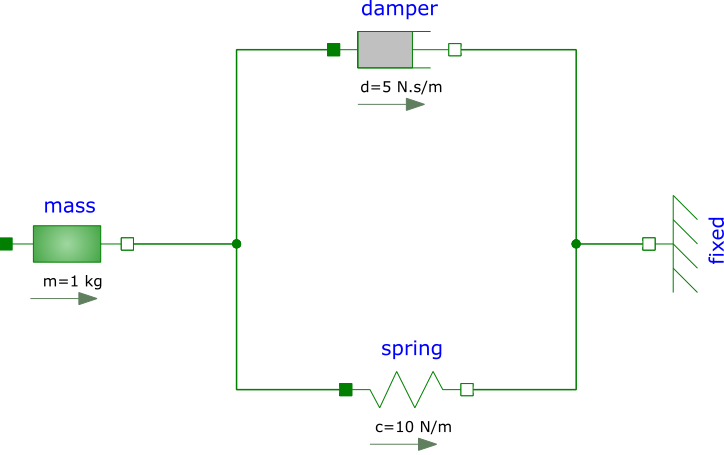
\includegraphics[width=1\textwidth]{img/Example.png} 
	
	\vspace{1em} % Adds spacing between image and quote
	
	\caption[Modelo de ejemplo en Modelica]{Gráfico de bloques de un sistema resorte-amortiguador creado y exportado como SVG desde OpenModelica.}
	\label{fig:example}
\end{figure}




\newpage

\begin{lstlisting}[caption={Código del ejemplo resorte-amortiguador}, label={lst:example}]
model Example
	Modelica.Mechanics.Translational.Components.Mass mass(m = 1);
	Modelica.Mechanics.Translational.Components.Fixed fixed;
	Modelica.Mechanics.Translational.Components.Damper damper(d = 5);
	Modelica.Mechanics.Translational.Components.Spring spring(s_rel(start = 0), c = 10, s_rel0 = 2);
equation
	connect(mass.flange_b, damper.flange_a);
	connect(damper.flange_b, fixed.flange;
	connect(spring.flange_a, mass.flange_b);
	connect(spring.flange_b, fixed.flange);
end Example;
\end{lstlisting}

En la figura~\ref{fig:example} se muestra un modelo de ejemplo desarrollado en OpenModelica, representa a una masa de $1$ kg conectada a un sistema resorte-amortiguador de una dimensión. El modelo está compuesto de otros modelos que se usan como base, particularmente, se están utilizando los modelos \textit{Mass}, \textit{Damper}, \textit{Spring} y \textit{Fixed}. Cada uno de estos modelos tiene sus ecuaciones constitutivas, y se conectan entre ellos mediante conectores denominados \textit{flange} (en el caso de un sistema de una dimensión translacional). \\

El gráfico representa la \textit{Diagram View} o vista de diagrama, que es una herramienta visual para crear modelos en la cual los objetos simplemente se arrastran al diagrama y se conectan de forma interactiva, sin embargo, esto es solamente una interfaz gráfica que funciona como frente ante el código en Modelica. El código~\ref{lst:example} es la traducción de la figura~\ref{fig:example} a lenguaje Modelica, esto se hace automáticamente y ambas representaciones son equivalentes y válidas por sí mismas. Este lenguaje utiliza un paradigma orientado a objetos, lo que hace sencillo importar y utilizar los elementos de la librería mencionados anteriormente. \\

Tanto el gráfico como el código orientado a objetos son una forma de facilitar el modelado para el usuario, luego, el compilador se encarga de procesar el modelo para obtener código ejecutable, el cual corre la simulación. En el caso de OpenModelica, el compilador OMC se organiza en cuatro etapas: un \textit{frontend}, un \textit{backend} de optimización simbólica, una etapa de generación de código y los entornos de ejecución (\textit{runtimes}) \cite{om_compiler}. \\

\subsubsection{Frontend y aplanamiento} 




Primero, el código pasa por las etapas clásicas de un compilador: análisis léxico, análisis sintáctico y análisis semántico. El árbol resultante de las etapas anteriores se traduce a una representación intermedia denominada SCode, que el \textit{frontend} continúa procesando hasta obtener una representación DAE del modelo \cite{om_compiler}. En este proceso se realiza el aplanamiento o \textit{flattening}, que produce una representación plana del modelo que contiene solamente declaraciones de variables, funciones, registros y ecuaciones. Todos los elementos de un lenguaje orientado a objetos se eliminan \cite{om_flattening}. Cada conexión entre componentes se reemplaza por otras generadas automáticamente a partir de las definiciones de dicho modelo. El resultado es un sistema DAE implícito como el de la ecuación~\eqref{eq:example_flat}, que en modelos multicuerpo puede alcanzar las miles de ecuaciones.

\begin{subequations}
	\label{eq:example_flat}
	\begin{align}
		% --- Ecuaciones generadas por las conexiones ---
		s_{k,a} &= s_{m,b}, & s_{k,a} &= s_{d,a}, \label{eq:flat_conn_first}\\
		s_{k,b} &= s_{F},   & s_{k,b} &= s_{d,b}, \\
		f_{m,a} &= 0, & f_{k,a} + f_{d,a} + f_{m,b} &= 0, \\
		& & f_{k,b} + f_{d,b} + f_{F} &= 0, \label{eq:flat_conn_last}\\[4pt]
		% --- Masa ---
		v_m &= \dot{s}_m, & a_m &= \dot{v}_m, \\
		m\, a_m &= f_{m,a} + f_{m,b}, & & \\
		s_{m,a} &= s_m - \tfrac{L}{2}, & s_{m,b} &= s_m + \tfrac{L}{2}, \\[4pt]
		% --- Soporte fijo ---
		s_F &= s_0, & & \\[4pt]
		% --- Amortiguador ---
		f_d &= d\, v_d, & P_d &= f_d\, v_d, \\
		s_d &= s_{d,b} - s_{d,a}, & v_d &= \dot{s}_d, \\
		f_{d,b} &= f_d, & f_{d,a} &= -f_d, \\[4pt]
		% --- Resorte ---
		f_k &= c\,\bigl(s_k - s_{k0}\bigr), & s_k &= s_{k,b} - s_{k,a}, \\
		f_{k,b} &= f_k, & f_{k,a} &= -f_k.
	\end{align}
\end{subequations}

\begin{table}[H]
	\centering
	\small
	\begin{tabularx}{\linewidth}{@{}l >{\raggedright\arraybackslash}X >{\raggedright\arraybackslash}X@{}}
		\hline
		Símbolo & Variable en OpenModelica & Descripción \\ \hline
		$s_m,\ v_m,\ a_m$ & \texttt{mass.s}, \texttt{mass.v}, \texttt{mass.a} & Posición, velocidad y aceleración de la masa \\
		$m,\ L$ & \texttt{mass.m}, \texttt{mass.L} & Masa y longitud \\
		$s_d,\ v_d$ & \texttt{damper.s\_rel}, \texttt{damper.v\_rel} & Elongación y velocidad relativa del amortiguador \\
		$f_d,\ P_d,\ d$ & \texttt{damper.f}, \texttt{damper.lossPower}, \texttt{damper.d} & Fuerza, potencia disipada y constante de amortiguamiento \\
		$s_k,\ f_k$ & \texttt{spring.s\_rel}, \texttt{spring.f} & Elongación y fuerza del resorte \\
		$c,\ s_{k0}$ & \texttt{spring.c}, \texttt{spring.s\_rel0} & Rigidez y longitud natural del resorte \\
		$s_0,\ s_F,\ f_F$ & \texttt{fixed.s0}, \texttt{fixed.flange.s}, \texttt{fixed.flange.f} & Posición y fuerza del soporte fijo \\
		$s_{i,j},\ f_{i,j}$ & \texttt{<comp>.flange\_<j>.s/f} & Posición y fuerza en la brida $j$ del componente $i$ \\ \hline
	\end{tabularx}
	\caption{Nomenclatura del ejemplo masa-resorte-amortiguador.}
	\label{tab:example_nomenclature}
\end{table}

\subsubsection{Backend: optimización simbólica} 
El \textit{backend} transforma ese sistema en una forma apta para la integración numérica, aplicando los algoritmos descritos en la sección~\ref{sec:dae_section}. Este paso se divide en tres fases \cite{om_compiler}:
\begin{itemize}
	
	
	\item \textbf{Preoptimización:} Particiona el sistema y elimina variables alias. Las ecuaciones triviales del tipo $a = b$ se descartan conservando una sola de las variables, la cual reemplaza a la otra. En OMC esta tarea la realiza el módulo \texttt{removeSimpleEquations} \cite{om_flags}.
	
	\item \textbf{Causalización:} Hace el \textit{matching} que asigna a cada ecuación la variable que debe despejarse de ella (ordenamiento horizontal), el ordenamiento de ecuaciones en una secuencia ejecutable (ordenamiento vertical) y la reducción de índice \cite{om_compiler}.
	
	%\item \textbf{Causalización:} comprende el \textit{matching}, que asigna a cada ecuación la variable que debe despejarse de ella (el ordenamiento horizontal), el ordenamiento de las ecuaciones en una secuencia ejecutable (el ordenamiento vertical) y la reducción de índice \cite{om_compiler}. Por defecto, OMC reduce el índice mediante el método \texttt{dynamicStateSelection}, que selecciona dinámicamente qué variables actuarán como estados en función de un análisis del sistema; alternativamente, el método \texttt{dummyDerivatives} realiza una selección estática basada en heurísticas \cite{om_flags}. La selección dinámica responde a que, en sistemas mecánicos con lazos cinemáticos cerrados, puede no existir un único conjunto de variables de estado que resulte adecuado durante toda la simulación, por lo que la decisión se posterga hasta el tiempo de ejecución \cite{cellier2006}.
	\item \textbf{Postoptimización:} Aplica \textit{tearing} sobre los lazos algebraicos restantes y calcula los jacobianos \cite{om_compiler}.
	
	%\item \textbf{Postoptimización:} aplica \textit{tearing} sobre los lazos algebraicos remanentes y calcula los jacobianos \cite{om_compiler}. El \textit{tearing} selecciona un subconjunto de variables de iteración (variables de corte) tal que el resto de las ecuaciones del lazo pueda resolverse explícitamente a partir de ellas, dejando un sistema reducido de ecuaciones residuales. De esta forma disminuye el tamaño de los sistemas lineales y no lineales que deben resolverse, el tamaño de sus jacobianos y la cantidad de valores iniciales requeridos por el método de Newton \cite{om_solving, cellier2006}.
\end{itemize}

El resultado de ejecutar estos pasos sobre el modelo DAE descrito anteriormente es un sistema DAE explícito el bloque de la ecuación~\ref{eq:example_ode_sorted} permite calcular las derivadas de los estados y la ecuación~\ref{eq:example_alg_sorted} las salidas.

% Ecuaciones evaluadas por el integrador en cada paso (ordenadas)
\begin{subequations}
	\label{eq:example_ode_sorted}
	\begin{align}
		\dot{s}_d &\coloneqq v_d \\
		f_d       &\coloneqq d\, v_d \\
		s_{k,a}   &\coloneqq s_0 - s_d \\
		s_k       &\coloneqq s_0 - s_{k,a} \\
		f_k       &\coloneqq c\,\bigl(s_k - s_{k0}\bigr) \\
		f_F       &\coloneqq -f_k - f_d \\
		a_m       &\coloneqq -f_F / m \\
		\dot{v}_d &\coloneqq -a_m
	\end{align}
\end{subequations}

% Ecuaciones algebraicas evaluadas solo para las salidas
\begin{subequations}
	\label{eq:example_alg_sorted}
	\begin{align}
		\dot{s}_m &\coloneqq -v_d, & v_m &\coloneqq -v_d, \\
		\dot{s}_{k,a} &\coloneqq -v_d, & P_d &\coloneqq f_d\, v_d, \\
		s_m &\coloneqq s_{k,a} - \tfrac{L}{2}, & s_{m,a} &\coloneqq s_m - \tfrac{L}{2}, \\
		\ddot{s}_{k,a} &\coloneqq a_m, & \dot{v}_m &\coloneqq a_m, \\
		f_{m,b} &\coloneqq -f_F. & &
	\end{align}
\end{subequations}

\subsubsection{Generación de código y ejecución}
A partir de la representación optimizada el compilador genera código en C o C++ y compila el resultado en un ejecutable de simulación \cite{om_compiler}. Por defecto, OpenModelica transforma el modelo a una representación ODE y la integra numéricamente. Los lazos algebraicos que el \textit{tearing} no pudo eliminar se resuelven en cada evaluación del modelo mediante \textit{solvers} lineales y no lineales. Además, OpenModelica ofrece un modo DAE, en el que el sistema completo de ecuaciones, incluidos sus lazos algebraicos, se entrega directamente al integrador IDA de la suite SUNDIALS \cite{om_solving}.


 %El paso central de este proceso es el \textit{aplanamiento} (\textit{flattening}), que produce una representación plana del modelo que contiene únicamente declaraciones de variables, funciones y registros, ecuaciones y ecuaciones iniciales. Todas las características orientadas a objetos del lenguaje, como la búsqueda de nombres, la instanciación, la herencia y las conexiones, desaparecen en esta representación \cite{om_flattening}. En particular, cada conexión entre componentes se reemplaza por ecuaciones generadas automáticamente a partir de la topología del modelo, de modo que muchas de las ecuaciones del sistema final no fueron escritas explícitamente por el modelador \cite{cellier2006}. El resultado es un sistema DAE implícito como el de la Ecuación~\eqref{eq:implicit_dae}, que en modelos multicuerpo puede alcanzar fácilmente miles de ecuaciones.







%La traducción y resolución de estos modelos se llevará a cabo mediante OpenModelica, un entorno de desarrollo de código abierto mantenido por el \textit{Open Source Modelica Consortium} (OSMC). La elección de esta plataforma se fundamenta en su naturaleza libre y gratuita, atributo que permite el acceso a herramientas de simulación de grado industrial para desarrolladores independientes e instituciones académicas. Dentro de este ecosistema, el proyecto se apoyará principalmente en dos componentes: el OMC (\textit{OpenModelica Compiler}), cuyo núcleo se encarga de analizar, optimizar y traducir el código Modelica a lenguaje C para su compilación final; y OMEdit, una interfaz gráfica de usuario (GUI) que facilita la creación, edición y visualización topológica de los modelos.\\

\section{Biblioteca \textit{MultiBody}}
Como base estructural para el desarrollo del modelo, se empleará la biblioteca \textit{MultiBody} de Modelica, perteneciente a la Modelica Standard Library. Esta biblioteca proporciona un conjunto de modelos predefinidos para componentes mecánicos tridimensionales, los cuales se interconectan utilizando un conector común, el marco de referencia \cite{msl_multibody}. Estos elementos actuarán como los bloques de construcción fundamentales del proyecto, los cuales serán interconectados, parametrizados y, en caso de ser necesario, extendidos para representar la topología cinemática y el comportamiento dinámico de los distintos subsistemas del vehículo.\\

Adicionalmente, la biblioteca \textit{MultiBody} incluye un motor de animación 3D integrado que permite la visualización geométrica de las partes mecánicas directamente dentro del entorno de OpenModelica  \cite{msl_multibody}. Si bien esta herramienta nativa resultará valiosa durante las etapas tempranas de desarrollo para la verificación de la correctitud de la cinemática y la ejecución de pruebas automatizadas de validación, presenta limitaciones significativas para el objetivo final del proyecto. Al estar diseñada principalmente para el análisis de ingeniería estático o precalculado, su motor de renderizado no está optimizado para garantizar la baja latencia que exige una simulación interactiva. Por este motivo, su uso se restringirá exclusivamente a la validación teórica del modelo físico, delegando la retroalimentación visual del usuario en tiempo real al motor gráfico Unity. \\

\subsection{Componentes de la biblioteca \textit{MultiBody}}

A continuación se van a detallar los componentes de la librería \textit{MultiBody} que son relevantes para comprender los modelos desarrollados en esta tesina. Toda la información sobre ellos se toman de la documentación oficial de la \textit{Modelica Standard Library} \cite{msl_multibody, otter2003}.

\subsection*{Sistema de referencia y conectores}



\subsubsection{Frame\_a / Frame\_b} 
El conector \verb|Frame| es el elemento sobre el cual se construyen los modelos multicuerpos. Representa un marco de referencia unido a un punto de un cuerpo, y transporta cuatro variables  \cite{msl_multibody}: el vector de posición \verb|r_0| que contiene las coordenadas \textit{x}, \textit{y} y \textit{z}, con respecto al origen del marco global (\textit{world}), resuelto con respecto a este, el objeto de orientación \verb|R|, que describe la rotación y dirección del conector, también con respecto al marco global y la fuerza \verb|f| y el torque \verb|t| resueltos en el marco del conector. Las dos primeras variables son de esfuerzo (\textit{potential}) y las dos últimas son variables de flujo (\textit{flow}), esta estructura es la que permite la conexión física: al conectar dos marcos, se igualan las posiciones y orientaciones, mientras que las fuerzas y torques se igualan a cero, respetando la tercera ley de Newton.  Las variantes \verb|Frame_a| (icono relleno) y \verb|Frame_b| (icono sin rellenar) son idénticas en contenido y solo se distinguen gráficamente para indicar la convención de conexión \cite{msl_multibody}.



\subsubsection{World}
El modelo \verb|World| define el marco de referencia global y el campo de gravedad uniforme del entorno de la simulación, además de los ajustes de animación por defecto. Todo modelo multicuerpo debe contener exactamente una instancia de \verb|World| para que todos los componentes estén sincronizados. Esta instancia debe ser declarada como objeto \texttt{inner}, para que el resto de los componentes puedan acceder a la gravedad y parámetros de visualización compartidos mediante la referencia \texttt{outer}.

\subsection*{Cuerpos e inercias}



\subsubsection{Body} 
Modela un cuerpo rígido usando un único marco de referencia \verb|frame_a|. Se parametriza mediante la masa $m$ (kg), la posición del centro de masa \verb|r_CM| relativa a \verb|frame_a| y las componentes del tensor de inercia. Se utiliza este componente cuando la geometría del cuerpo no es relevante y solo se necesitan sus propiedades inerciales, como en la masa de los neumáticos.



\subsubsection{BodyBox / BodyCylinder} 
Son cuerpos rígidos que poseen una forma geométrica dada, la de un paralelepípedo y un cilindro (opcionalmente hueco) respectivamente. Estos componentes calculan automáticamente la masa y el tensor de inercia completo a partir de las dimensiones geométricas y la densidad del material \cite{msl_multibody}. A diferencia de \verb|Body|, estos exponen dos marcos de referencia  (\verb|frame_a| y \verb|frame_b|) en sus extremos, permitiendo que se puedan insertar como eslabones en una cadena. La geometría de \verb|BodyBox| resulta útil para abstraer la distribución del peso de un chasis, mientras que \verb|BodyCylinder| se utiliza por la misma razón en los brazos de suspensión.



\subsubsection{FixedTranslation}
Representa una traslación rígida y sin masa que posiciona el vector de posición $r$ entre \verb|frame_a| y \verb|frame_b|, manteniendo ambos marcos con la misma orientación. Se utiliza para definir los puntos de montaje, por ejemplo: anclajes de suspensión, \textit{offsets} de rueda sin añadir inercia al sistema.


\subsection*{Articulaciones (\textit{Joints})}



\subsubsection{Revolute} 
Articulación de rotación sobre un único grado de libertad: el ángulo de giro $\varphi$ alrededor de un eje $n$ fijo en \verb|frame_a|. Cuando se activa la opción \verb|useAxisFlange|, expone una brida rotacional unidimensional (\verb|axis|) que permite alterar el giro (por ejemplo, iniciando, frenando o bloqueando), acoplando de esa forma el dominio mecánico tridimensional con el rotacional de una dimensión. Se utiliza como la base de los giros de las ruedas y de los pivotes de dirección.

\subsubsection{Prismatic} 
Articulación de traslación con un solo grado de libertad: el desplazamiento relativo $s$ a lo largo de un eje $n$. Al igual que \verb|Revolute|, admite una brida opcional. Se utiliza para modelar el recorrido vertical de la suspensión \verb|McPherson|.



\subsubsection{FreeMotion} 
Articulación con los seis grados de libertad (tres traslacionales y tres rotacionales), que describe el movimiento libre de \verb|frame_b| respecto de \verb|frame_a|. Se utiliza para conectar al chasis con el mundo sin imponer restricciones cinemáticas, la posición y velocidad relativas actúan como variables de estado, lo que permite fijar condiciones iniciales como la posición del vehículo al iniciar la simulación.



\subsubsection{JointRRR} 
Pertenece al subpaquete \verb|Joints.Assemblies| y agrega tres articulaciones de revolución con ejes de rotación paralelos, conectadas entre sí por dos barras rígidas, formando así, un bucle cinemático plano \cite{msl_multibody}. Su característica principal es que no introduce restricciones ni variables de estado, sino que resuelve analíticamente la cinemática no lineal del bucle a partir de la posición y orientación de \verb|frame_a| y \verb|frame_b|. La documentación oficial recomienda su uso en los bucles cinemáticos siempre que sea posible, para evitar sistemas de ecuaciones no lineales \cite{msl_multibody}. Además de \verb|frame_a| y \verb|frame_b|, disponibiliza los marcos interiores \verb|frame_ia|, \verb|frame_im| y \verb|frame_ib|, y su geometría se define mediante los vectores de barra \verb|rRod1_ia| y \verb|rRod2_ib|. Este componente es el que hace posible modelar las suspensiones \verb|DoubleWishbone| y \verb|MultiLink| sin degradar la eficiencia numérica y evitando fallos a la hora de ejecutar la simulación.

\subsection*{Elementos de fuerza}

\subsubsection{SpringDamperParallel} 
Elemento de fuerza que conecta un resorte lineal en paralelo con un amortiguador lineal, actuando a lo largo de la recta definida por \verb|frame_a| y \verb|frame_b|. Sus parámetros se componen de la constante de rigidez $c$, el coeficiente de amortiguamiento $d$ y la longitud sin estirar \verb|s_unstretched|. La fuerza resultante a lo largo de la línea de acción es $f = c\,(s - s_0) + d\,\dot{s}$, siendo $s$ la distancia entre \verb|frame_a| y \verb|frame_b|. Constituye la base de todos los conjunto resorte-amortiguador de la suspensión.

\subsubsection{WorldForce / WorldForceAndTorque}
Aplican un vector de fuerza y adicionalmente un vector de torque, respectivamente, sobre el marco al que se conectan, resueltos en el marco global. Se emplean para agregar en el modelo las fuerzas de contacto con el suelo y la fricción calculados en el paquete \verb|Roads|.

\subsection*{Visualización}


\subsubsection{Visualizers}
La biblioteca \textit{MultiBody} incorpora componentes exclusivamente gráficos que no aplican fuerzas ni torques. La clase base \verb|PartialVisualizer| y los modelos \verb|Advanced.Shape| y \verb|Advanced.Surface| renderizan formas geométricas (cajas, cilindros u otras superficies arbitrarias) siguiendo la posición y orientación de un marco de referencia. Se utilizan para representar visualmente el terreno, los neumáticos y demás elementos en el motor de animación 3D de OpenModelica.\\\\

Vale la pena mencionar que los subsistemas de transmisión, dirección y frenado emplean elementos de la biblioteca \textit{Modelica.Mechanics.Rotational}, que contiene elementos de mecánica rotacional unidimensionales, tales como los conectores de brida (\verb|Flange_a|, \verb|Flange_b|), las fuentes de posición y par (\verb|Sources.Position|, \verb|Sources.Torque|), el sensor de velocidad (\verb|Sensors.SpeedSensor|) y el anclaje fijo (\verb|Components.Fixed|), que se acoplan al dominio tridimensional mediante la brida de eje de las articulaciones \verb|Revolute| y \verb|Prismatic|.

\section{Biblioteca \textit{Modelica\_DeviceDrivers}}

Para la comunicación entre el modelo Modelica y los sistemas externos (el visualizador y el puente de hardware) se emplea la biblioteca \textit{Modelica\_DeviceDrivers} (MDD), una biblioteca de código abierto destinada a interconectar controladores de hardware y protocolos de comunicación con modelos de Modelica \cite{mdd}. De ella se utilizaron componentes de tres grupos funcionales: el empaquetado serializado de datos, la comunicación por UDP y la sincronización con el tiempo real. Estos bloques son los que materializan los modelos del paquete \verb|Interfaces| descritos más adelante. Toda la información sobre los modelos que se describen a continuación se obtuvo de la documentación oficial \cite{mdd_docs}.

\subsection*{Empaquetado de datos (\textit{SerialPackager})}

El subpaquete \verb|Packaging.SerialPackager| resuelve la serialización de datos en un formato binario transmisible para la comunicación por red. Según la documentación oficial, el objetivo del \textit{SerialPackager} es permitir agregar y recuperar datos de un paquete de manera independiente del dispositivo \cite{mdd}. Los bloques se encadenan a través de conectores (\verb|pkgIn| y \verb|pkgOut|) que representan un buffer de paquete a compartir, el cual va siendo construido o desarmado a medida que se recorre la cadena.


\subsubsection{Packager}
Es el bloque de cabecera de la cadena: inicializa el búfer del paquete sobre el que los bloques posteriores escriben o del que leen.

\subsubsection{AddFloat}

Toma un vector de valores \verb|Real| y los convierte en un número de punto flotante de $32$ bits para luego añadirlos al paquete. El parámetro \verb|nu| indica el número de entradas. Se emplea del lado emisor para serializar las coordenadas y/o señales.



\subsubsection{GetFloat} 
Realiza la operación inversa a \verb|AddFloat|, extrae un vector de números de punto flotante del paquete recibido y los convierte a doble precisión antes de asignarlo a un arreglo \verb|Real| de Modelica \cite{mdd}. Se emplea del lado receptor para obtener las señales entrantes

\subsection*{Comunicación por UDP}

El subpaquete \verb|Communication| provee los bloques de entrada y salida de red que transportan el paquete serializado a través del protocolo UDP.



\subsubsection{UDPSend}
Bloque que permite el envío de datagramas UDP hacia la red. Recibe el paquete ensamblado a través de su conector \verb|pkgIn| y lo emite como un datagrama hacia el puerto \verb|port_send| con un período definido por \verb|sampleTime|. Es el bloque final de la cadena de transmisión.



\subsubsection{UDPReceive}
Bloque que permite la recepción de datagramas UDP. Escucha en el puerto definido por \verb|port_recv|, mediante un hilo de recepción en el segundo plano y expone los bytes serializados recibidos a través de su conector \verb|pkgOut| para que luego los bloques \verb|GetFloat| los desempaqueten. Es el bloque inicial de la cadena de recepción.

\subsection*{Sincronización con el tiempo real}



\subsubsection{RealtimeSynchronize}
Este bloque se encarga de la sincronización del tiempo de la simulación con el reloj de tiempo real del sistema operativo. Su funcionamiento consiste en comparar, mediante una función externa en C, el tiempo de simulación con el reloj del sistema, deteniendo la ejecución del hilo hasta que el primero alcanza al segundo. Es indispensable para que una simulación que podría ejecutarse más rápido que el tiempo real se ajuste al ritmo del mundo físico, condición necesaria tanto para una visualización fiel, como para cerrar el feedback del conductor. La documentación advierte de que se trata de una sincronización blanda (\textit{soft real-time}) no apta para aplicaciones de tiempo real estricto ni de seguridad crítica \cite{mdd}, pero para un simulador de conducción interactivo, esta aproximación me pareció suficiente. El bloque admite además un modo muestreado (\textit{sampled}) que ofrece un comportamiento más determinista y menos sensible al solver.

En conjunto, estos bloques se utilizan en dos sentidos:  en la transmisión, \verb|Packager| $\rightarrow$ \verb|AddFloat| (uno por señal) $\rightarrow$ \verb|UDPSend|, y en la recepción, \verb|UDPReceive| $\rightarrow$ \verb|GetFloat| (uno por señal), todo ello sincronizado por \verb|RealtimeSynchronize|.


\section{Visualizadores}
Para realizar el entorno de interacción entre el modelo matemático y el usuario, resulta fundamental contar con una herramienta de visualización capaz de recibir, procesar y renderizar los datos del vehículo de forma fluida y con latencia baja. En la industria de la simulación profesional existen plataformas dedicadas a este propósito, tales como rFpro o las versiones profesionales de Assetto Corsa. Sin embargo, estas soluciones son de carácter propietario e involucran costos de licencia prohibitivos para la investigación independiente. Adicionalmente, al ser plataformas integrales, presentan características que resultan redundantes o irrelevantes para este trabajo, el cual requiere estrictamente un motor de representación gráfica externo.
\\

Para el desarrollo de esta tesina se seleccionó el motor gráfico Unity como entorno de visualización. Esta elección se fundamenta en su arquitectura flexible, su extensa documentación técnica y, principalmente, su capacidad nativa para integrarse de manera eficiente con bibliotecas externas (a través de scripts y protocolos de red). Utilizando esta plataforma, se implementará un entorno tridimensional que actuará como cliente visualizador, el cual estará dedicado exclusivamente a interpretar el flujo de datos telemétricos provenientes de Modelica y reflejar, en tiempo real estricto, el estado dinámico del vehículo y su posicionamiento espacial dentro del entorno virtual. \\


\subsection{El motor gráfico Unity}

%Unity es un motor gráfco de desarrollo multiplataforma para aplicaciones interactivas en tiempo real
La arquitectura de Unity se organiza en torno a algunos conceptos fundamentales, definidos en su documentación oficial \cite{unity_docs}, que resultan necesarios para comprender la interfaz desarrollada:

\begin{itemize}
	\item \textbf{Escena y \textit{GameObjects}.} Una escena contiene un conjunto de objetos (\textit{GameObjects}), que son los contenedores básicos de todo elemento del mundo virtual, en este caso se utilizan para el chasis y las cuatro ruedas del auto.
	
	\item \textbf{Componente \textit{Transform}.} Cada \textit{GameObject} posee un componente \verb|Transform| que almacena la posición, rotación, escala y estado de jerarquía del objeto. Al modificar este componente, el objeto puede reposicionarse y reorientarse en la escena.
	
	\item \textbf{\textit{MonoBehaviour} y \textit{scripts}.} El comportamiento programable de un objeto se agrega mediante \textit{scripts} escritos en C\# que derivan de la clase base \verb|MonoBehaviour|. Esta clase expone una serie de funciones de ciclo de vida que el motor invoca automáticamente, como \verb|Start| (inicialización) y \verb|FixedUpdate| (actualización por intervalo).
	
	
	\item \textbf{Bucle de física \textit{FixedUpdate}.} A diferencia de \verb|Update|, que se ejecuta una vez por fotograma renderizado y por lo tanto su frecuencia varía dependiendo del rendimiento del computador, \verb|FixedUpdate| se invoca a intervalos fijos como parte del bucle de física del motor \cite{unity_docs}, lo que garantiza un ritmo de actualización determinista, independiente de la tasa de refresco gráfico.
	
	
	\item \textbf{Sistema de coordenadas.} Unity emplea un sistema de coordenadas levógiro (sentido antihorario) con el eje $Y$ apuntando hacia arriba, y representa las rotaciones internamente como cuaterniones. Esta convención difiere de la de Modelica, que es dextrógira (sentido horario) y también con $Y$ vertical, discrepancia que la interfaz debe resolver explícitamente.
\end{itemize}


\section{Simulaciones Man-In-The-Loop}
El término simulación \textit{Man-in-the-Loop} (MITL), también denominado \textit{Human-in-the-Loop} (HITL) o, en el contexto específico de la simulación automotriz, \textit{Driver-in-the-Loop} (DIL), hace referencia a aquellos entornos de simulación que integran de forma activa y directa a un humano dentro del control del sistema. En estas arquitecturas, las acciones del usuario modifican dinámicamente las variables de estado y la evolución del modelo físico. Este enfoque se vuelve indispensable cuando las decisiones, reacciones y comportamientos del operador presentan un grado de variabilidad que resulta complejo de replicar mediante algoritmos deterministas o modelos matemáticos.\\

La inclusión del factor humano en tiempo real permite que el usuario altere el curso y el resultado de un proceso o evento simulado. El nivel de inmersión y fidelidad que ofrecen estos entornos contribuye de manera efectiva a una transferencia de las habilidades y reflejos adquiridos en el entorno virtual hacia el mundo real. \\

Asimismo, a diferencia de los modelos de simulación completamente automatizados, el paradigma \textit{Human-in-the-Loop} es el único capaz de reproducir y evaluar el impacto del error humano, la fatiga y los tiempos de reacción ante situaciones críticas o límites. A pesar de los esfuerzos actuales por automatizar sistemas complejos, el juicio, la percepción sensorial y la experiencia del conductor siguen siendo componentes críticos. En este tipo de simulación interactiva, el operador procesa la información y los estímulos provistos por la plataforma (como la retroalimentación visual y de fuerzas) para determinar el siguiente curso de acción en fracciones de segundo, cerrando así un ciclo de retroalimentación.


\section{Trabajos Anteriores}
En la actualidad, el lenguaje Modelica se ha consolidado como un estándar en la industria automotriz para el desarrollo de simuladores. Grandes fabricantes del sector, tales como Honda, Rimac y BMW, emplean esta tecnología para modelar la dinámica de sus vehículos \cite{modelon}. No obstante, estas implementaciones suelen depender de ecosistemas cerrados que incluyen bibliotecas propietarias y compiladores comerciales de alto costo, como es el caso de Dymola. Si bien existen investigaciones previas y artículos académicos que demuestran la viabilidad de utilizar estas bibliotecas para definir sistemas complejos en tiempo real \cite{modelicart}, el acceso a dichas herramientas representa una barrera para investigadores independientes o desarrolladores con recursos limitados. Este proyecto tiene el objetivo de recrear una alternativa de código abierto que permita el acceso a estas capacidades de simulación, permitiendo su uso y extensión por parte de una comunidad más amplia. \\

Se identificó una publicación con objetivos similares a los de este trabajo \cite{modelica2003}. Sin embargo, esta implementación data de hace más de dos décadas, lo que conlleva problemas de compatibilidad con versiones modernas de OpenModelica y con los estándares actuales del lenguaje. El desfase tecnológico también omite avances recientes en métodos de integración numérica y optimización de modelos que son importantes para la estabilidad en tiempo real. \\

En cuanto a la interacción con el sistema, se cuenta con el hardware de simulación necesario para actuar como periférico de entrada. Para la gestión de estos dispositivos, se utilizarán las bibliotecas SDL \cite{sdl} y DirectInput \cite{di}. La elección de estas herramientas permite mantener una estandarización con los periféricos y softwares de simulación comercial actuales. Esto garantiza que el sistema desarrollado sea compatible con una amplia gama de volantes, pedaleras y palancas de cambio de grado profesional y comercial, asegurando una experiencia de usuario consistente con los estándares de la industria.

% Contributions
\chapter{Desarrollo}
\label{sec:method}
%\section{Componentes de la biblioteca \textit{MultiBody}}

%Antes de detallar la arquitectura de la biblioteca desarrollada, resulta conveniente describir los componentes de la biblioteca estándar \textit{MultiBody} que se emplearon como bloques de construcción fundamentales. Todos ellos se toman de la documentación oficial de la \textit{Modelica Standard Library} \cite{msl_multibody, otter2003}. La biblioteca \textit{MultiBody} proporciona modelos de componentes mecánicos tridimensionales (cuerpos rígidos, articulaciones y elementos de fuerza) que se interconectan de a través de un conector común, el marco de referencia.


\section{Componentes de la biblioteca \textit{Modelica\_DeviceDrivers}}

Para la comunicación entre el modelo Modelica y los sistemas externos (el visualizador y el puente de hardware) se emplea la biblioteca \textit{Modelica\_DeviceDrivers} (MDD), una biblioteca libre destinada a interconectar controladores de hardware y protocolos de comunicación con modelos de Modelica \cite{mdd}. De ella se utilizaron componentes de tres grupos funcionales: el empaquetado serializado de datos, la comunicación por UDP y la sincronización con el tiempo real. Estos bloques son los que materializan los modelos del paquete \verb|Interfaces| descritos más adelante.

\subsection*{Empaquetado de datos (\textit{SerialPackager})}

El subpaquete \verb|Packagin.SerialPackager| resuelve la serialización de datos en un formato binario transmisible para la comunicación por red. Según la documentación oficial, el objetivo del \textit{SerialPackager} es permitir agregar y recuperar datos de un paquete de manera independiente del dispositivo \cite{mdd}. Los bloques se encadenan a través de conectores (\verb|pkgIn| y \verb|pkgOut|) que representan un buffer de paquete a compartir, el cual va siendo construido o desarmado a medida que se recorre la cadena.


\subsubsection{Packager}
Es el bloque de cabecera de la cadena: inicializa el búfer del paquete sobre el que los bloques posteriores escriben o del que leen.

\subsubsection{AddFloat}

Toma un vector de valores \verb|Real| y los convierte en un número de punto flotante de $32$ bits para luego añadirlos al paquete. El parámetro \verb|nu| indica el número de entradas. Se emplea del lado emisor para serializar las coordenadas y/o señales.



\subsubsection{GetFloat} 
Realiza la operación inversa a \verb|AddFloat|, extrae un vector de números de punto flotante del paquete recibido y los convierte a doble precisión antes de asignarlo a un arreglo \verb|Real| de Modelica \cite{mdd}. Se emplea del lado receptor para obtener las señales entrantes

\subsection*{Comunicación por UDP}

El subpaquete \verb|Communication| provee los bloques de entrada y salida de red que transportan el paquete serializado a través del protocolo UDP.



\subsubsection{UDPSend}
Bloque que permite el envío de datagramas UDP hacia la red. Recibe el paquete ensamblado a través de su conector \verb|pkgIn| y lo emite como un datagrama hacia el puerto \verb|port_send| con un período definido por \verb|sampleTime|. Es el bloque final de la cadena de transmisión.



\subsubsection{UDPReceive}
Bloque que permite la recepción de datagramas UDP. Escucha en el puerto definido por \verb|port_recv|, mediante un hilo de recepción en el segundo plano y expone los bytes serializados recibidos a través de su conector \verb|pkgOut| para que luego los bloques \verb|GetFloat| los desempaqueten. Es el bloque inicial de la cadena de recepción.

\subsection*{Sincronización con el tiempo real}



\subsubsection{RealtimeSynchronize}
Este bloque se encarga de la sincronización del tiempo de la simulación con el reloj de tiempo real del sistema operativo. Su funcionamiento consiste en comparar, mediante una función externa en C, el tiempo de simulación con el reloj del sistema, deteniendo la ejecución del hilo hasta que el primero alcanza al segundo. Es indispensable para que una simulación que podría ejecutarse más rápid que el tiempo real se ajuste al ritmo del mundo físico, condición necesaria tanto para una visualización fiel, como para cerrar el feedback del conductor. La documentación advierte de que se trata de una sincronización blanda (\textit{soft real-time}) no apta para aplicaciones de tiempo real estricto ni de seguridad crítica \cite{mdd}, pero para un simulador de conducción interactivo, esta aproximación me pareció suficiente. El bloque admite ademas un modo muestreado (\textit{sampled}) que ofrece un comportamiento más determinista y menos sensible al solver.

En conjunto, estos bloques se utilizan en dos sentidos:  en la transmisión, \verb|Packager| $\rightarrow$ \verb|AddFloat| (uno por señal) $\rightarrow$ \verb|UDPSend|, y en la recepción, \verb|UDPReceive| $\rightarrow$ \verb|GetFloat| (uno por señal), todo ello sincronizado por \verb|RealtimeSynchronize|.

\section{Biblioteca de dinámica vehicular}

En esta sección se explicará el desarrollo y arquitectura de la biblioteca de dinámica vehicular implementada en Modelica. Para garantizar la modularidad y facilitar el mantenimiento y evolución del código, la bilbioteca se organizó en tres paquetes principales:


\begin{itemize}
    \item \verb|Roads|: Contiene la lógica referida al entorno de la simulación, incluyendo características topológicas de la pista/circuito y la geometría de la superficie de contacto.
    \item \verb|Interfaces|: Define los conectores estandarizados y los protocolos de comunicación, permitiendo la comunicación fluida entre los diferentes subsistemas y la compatibilidad con componentes externos.
    \item \verb|Cars|: Agrupa los modelos físico-matemáticos correspondientes a la topología del vehículo, en este paquete se incluye el detalle de la cinemática del chasis, los sistemas de suspensión y demás elementos mecánicos estructurales, entre otras cosas.
\end{itemize}

\subsection{Interfaces}

El paquete \verb|Interfaces| actúa como capa de compatibilidad entre el dominio mecánico de la bibliotecta \textit{MultiBody} y los dominios de las señales de entrada del piloto y de la comunicación de red. Su función es tanto extraer información de estado del modelo físico y ponerla a disposición de otros subsistemas, ya sea como señales continuas internas o como datagramas transmitidos en tiempo real hacia un cliente externo mediante UDP, como permitir la recepción de señales pertenecientes a los inputs del vehículo, también mediantes datagramas UDP. Este paquete contiene dos familias de modelos: los que transmiten únicamente la posición (\verb|FrameToReal| y \verb|FrameToUDP|) y los que además transmiten la orientación del marco de referencia (\verb|FrameToRealOrientation| y \verb|FrameToUDPOrientation|), necesarios para reproducir en el visualizador la dirección del vehículo y el giro de las ruedas. A estos transmisores se suma un modelo de recepción, \verb|UDPInput|, que implementa el canal inverso: la lectura de los comandos del conductor enviados por la interfaz de hardware.\\

\subsubsection{FrameToReal}

El modelo \verb|FrameToReal| cumple con la función de sensor de posición sobre un conector \verb|Frame_a| de la biblioteca \textit{MultiBody}. Este marco transporta, entre sus componentes, el vector de posición en el sistema de referencia global $\mathbf{r}_0 \in \mathbb{R}^3$, así como las fuerzas y torques aplicados sobre este. Dado que el modelo tiene carácter observacional, las ecuaciones extraen las componentes cartesianas del vector de posición y las asignan a tres salidas de señal continua, de tipo \verb|Real|, sin aplicar ni fuerza ni torque sobre el frame, para garantizar que no se introducen variaciones inesperadas en el sistema::

\begin{align}
    x_{\text{out}} &= r_{0,1} \\
    y_{\text{out}} &= r_{0,2} \\
    z_{\text{out}} &= r_{0,3} \\
    \mathbf{f} &= \mathbf{0} \\
    \boldsymbol{\tau} &= \mathbf{0}
\end{align}

Las tres salidas son de tipo \verb|RealOutput| (pertenecientes a \verb|Modelica.Blocks.Interfaces|), lo que las hace directamente compatibles con cualquier bloque de procesamiento de señales del ecosistema Modelica.\\

\subsubsection{FrameToUDP}

El modelo \verb|FrameToUDP| construye sobre la funcionalidad de \verb|FrameToReal|, agregando una cadena de serialización y transmisión de datos por red basada en la biblioteca \verb|Modelica_DeviceDrivers|. Su objetivo es enviar la posición del vehículo a un cliente externo, en este caso, a el motor gráfico Unity, mediante el protocolo UDP, permitiendo la visualización en tiempo real del estado del sistema/vehículo. \\

Por dentro, el modelo encadena los siguientes componentes: \verb|FrameToReal| que extrae las tres coordenadas del marco de referencia como variables \verb|Real|, un bloque \verb|Packager| que inicializa el buffer del datagrama, tres instancias de \verb|AddFloat| que agregan cada coordenada como un número de punto flotante de 32 bits en formato IEEE 754 little-endian \cite{mdd}, finalmente, \verb|UDPSend| transmite el paquete resultante al puerto 12345 (configurable) con un período de muestreo de 
0{,}01 s, es decir a una frecuencia de 100Hz, esta frecuencia puede ser aumentada para mejorar la fidelidad de la simulación a cambio de necesitar más poder de procesamiento.

Como fue explicado en la sección de \textit{DeviceDrivers}, el paquete también incluye un componente adicional \verb|RealtimeSynchronize|, que sincroniza el reloj de la simulación con el reloj del sistema operativo. Esta sincronización es indispensable para que la frecuencia de los datagramas corresponda efectivamente a 100 paquetes (o lo configurado) por segundo en tiempo real, garantizando así, la coherencia entre el modelo de Modelica y el visualizador utilizado.\\

\subsubsection{FrameToRealOrientation}

Transmitir solamente la posición resulta insuficiente cuando se quiere representar la actitud del vehículo o el ángulo de dirección de las ruedas en el visualizador. El conector \verb|Frame_a| transporta, además del vector de posición $\mathbf{r}_0$ ya utilizado, un objeto de orientación $R$ que contiene la matriz de transformación $T \in \mathbb{R}^{3\times3}$ entre el sistema de referencia global y el sistema local del cuerpo. El modelo \verb|FrameToRealOrientation| extiende a \verb|FrameToReal| exponiendo, junto a las tres coordenadas de posición, dicha orientación en forma de cuaternión unitario.\\

Se optó por representar la orientación mediante un cuaternión y no por la matriz de rotación completa (nueve componentes) ni por ángulos de Euler, ya que el cuaternión requiere solo cuatro componentes, evita singularidades y es el formato nativo de rotación en Unity. La conversión se realiza con la función \verb|Frames.to_Q| de la biblioteca \textit{MultiBody}, que aplica la convención $\mathbf{Q} = [\sin(\theta/2)\,\hat{\mathbf{e}};\ \cos(\theta/2)]$, con la parte escalar en la última componente:

\begin{align}
    x_{\text{out}} &= r_{0,1} \\
    y_{\text{out}} &= r_{0,2} \\
    z_{\text{out}} &= r_{0,3} \\
    \mathbf{q}_{\text{out}} &= \text{to\_Q}(R) \\
    \mathbf{f} &= \mathbf{0} \\
    \boldsymbol{\tau} &= \mathbf{0}
\end{align}



Cabe destacar que $\text{to\_Q}(R)$, devuelve la rotación del cuerpo respecto del mundo expresada como cuaternión activo. El script que actúa como cliente receptor del lado de Unity convierte esta rotación al sistema de Unity aplicando la misma inversión de eje que a la posición, lo que equivale a negar las componentes $x$ e $y$ de la parte vectorial y conservar $z$ y $w$. Es importante destacar que negar la componente $z$ en su lugar produce la rotación inversa, lo que se ve reflejado como una representación errónea del movimiento del eje de giro de la rueda, cosa que fue una fuente de complicaciones durante el desarrollo.\\

\subsubsection{FrameToUDPOrientation}

El modelo \verb|FrameToUDPOrientation| es el equivalente a \verb|FrameToUDP| pero para la transmisión de la localización completa. Reemplaza el objeto \verb|FrameToReal| por \verb|FrameToRealOrientation| y amplía la cadena de serialización para incluír siete números en total de punto flotante en $32$ bits:
 las tres coordenadas de posición y las cuatro componentes del cuaternión. El puerto de destino (\verb|port_send|) y el período de muestreo (\verb|sampleTime|) se declaran como parámetros, lo que permite, además de intercambiar fidelidad por performace, instanciar varias transmisores al mismo tiempo, por ejemplo, incluyendo uno para el chasis y otros cuatro, uno para cada rueda, todos dirigidos a puertos distintos.\\

Cada valor se serializa mediante un bloque \verb|AddFloat| independiente encadenado en secuencia, en lugar de un único bloque configurado para siete valores. Esta decisión se tomó debido a una limitación observada en el compilador OpenModelica~1.25.5, en el que la modificación del parámetro de tamaño del bloque \verb|AddFloat| provoca un error interno de instanciación, el encadenamiento de bloques con el tamaño por defecto evita dicho comportamiento.\\

Dado que en la topología del vehículo los frames de las ruedas se ubican sobre la salida de la junta de rotación, la orientación transmitida incluye tanto el ángulo de dirección como el giro propio de la rueda, permitiendo que sea representada de forma correcta por el entorno gráfico. El ejemplo \verb|CarExampleUDP| demuestra este sistema, instanciando el vehículo y el entorno y aplicando una señal de dirección para probar el giro de la dirección y conecta cinco transmisores \verb|FrameToUDPOrientation| (chasis y cuatro ruedas) a puertos consecutivos del 12345 al 12349.\\

\subsubsection{UDPInput}

El modelo \verb|UDPInput| implementa el canal de comunicación de recepción del sistema, permitiendo obtener los comandos del conductor. Constituye la contraparte en Modelica de la aplicación de adquisición de datos desde el hardware descrita en la sección \textit{Interfaz para el hardware}, y cierra el lazo \textit{Man-in-the-Loop} al incluir en el modelo las acciones ejercidas por el piloto capturadas desde los periféricos.\\

Su estructura interna es simétrica a la de \verb|FrameToUDP|, pero orientada a la lectura: un bloque \verb|UDPReceive| escucha en el puerto configurable \verb|udpPort| (por defecto, 12347) y entrega el datagrama UDP recibido, para que luego, cuatro bloques \verb|GetFloat| desempaqueten la información y la codifiquen en cuatro números de punto flotante de $32$ bits, convirtiéndolos luego a variables \verb|Real| de doble precisión. Estas son expuestas como cuatro salidas \verb|RealOutput|: \verb|steer|, \verb|throttle|, \verb|brake| y \verb|clutch|, que se conectan respectivamente a las entradas \verb|steerInput|, \verb|throttleInput| y \verb|brakeInput| del modelo del vehículo (la señal de embrague queda disponible para usos futuros si se considerase necesaria). El formato de 16 bytes y el puerto 12347 coinciden exactamente con los que emite la aplicación \verb|FFBReceiver|, garantizando la conexión fluída entre ambos extremos. Al igual que los transmisores, incorpora un bloque \verb|RealtimeSynchronize| para sincronizar la recepción en tiempo real.\\

\subsection{Roads}

El paquete \verb|Roads| encapsula el entorno y el mundo de la simulación sobre el que opera el vehículo. Sus responsabilidades principales incluyen: por un lado, definir la geometría de la superficie de contacto que va a actuar como pista, y por otro, calcular y aplicar las fuerzas mecánicas generadas por la interacción entre cada neumático y dicha superficie. Este paquete se organiza en tres niveles: el modelo integrador \verb|Road|, el subpaquete \verb|Floor| que incluye los modelos de contacto entre la rueda y la superficie, y el subpaquete \verb|Terrains| que gestiona la definición y visualización del terreno.\\


\subsubsection{Road}

El modelo \verb|Road| es el componente de más alto nivel del paquete y actúa como punto de ensemble para el entorno completo. Instancia, primero, un objeto \verb|World| de la biblioteca \textit{MultiBody}, necesario para definir un sistema de referencia global y el vector de gravedad, junto con un \verb|TerrainMap| y un \verb|Floor4Corners|. Tanto \verb|World| como \verb|TerrrainMap| se declaran como objetos \texttt{inner}, lo que permite que cualquier submodelo del sistema los referencia mediante la palabra reservada \texttt{outer} sin necesidad de pasarlos como argumentos. \\

Hacia el resto del modelo, \verb|Road| expone cuatro conectores de tipo \verb|Frame_a|, uno perteneciente a cada esquina del vehículo: delantera izquierda (\verb|FL|), delantera derecha (\verb|FR|), trasera izquierda (\verb|RL|) y trasera derecha (\verb|RR|). Estos frames se conectan directamente con los de los centros de rueda del modelo del vehículo, constituyendo la conexión mecánica entre el entorno/mundo de simulación y el chasis.\\


\subsubsection{Floors}

El subpaquete \verb|Floors| implementa el modelo de contacto entre la rueda y el suelo mediante una jerarquía de tres clases. Arriba, \verb|Floor4Corners| agrega cuatro instancias del modelo \verb|Floor|, una por rueda, y les pasa a cada uno un conjunto de parámetros físicos compartidos: la rigidez del suelo \verb|ground_c| ($c = 10^5$ N/m), el coeficiente de amortiguamiento normal \verb|ground_d| ($d = 5000$ N$\cdot$s/m), el coeficiente de fricción longitudinal \verb|ground_mu| ($\mu_\text{long} = 10000$ N$\cdot$s/m) y el coeficiente de fricción lateral \verb|mu_lat| ($\mu_\text{lat} = 100000$ N$\cdot$s/m). El radio de la rueda \verb|R_wheel| se propaga hacia abajo mediante cláusulas \texttt{inner}/\texttt{outer} desde el nivel de simulación. \\

El modelo \verb|Floor| es un modelo compuesto que instancia dos subcomponentes, \verb|GroundSpring| y \verb|GroundFriction|, compartiando el mismo conector de contacto \verb|wheelContact|, de tipo \verb|Frame_b|. \\

\subsubsection{GroundSpring}
Este componente aplica la fuerza normal vertical, utilizando un modelo de resorte-amortiguador lineal. La fuerza aplicada es nula mientras el centro de la rueda (más su radio) se encuentre por encima de la superficie del terreno, y crece de forma proporcional a la profundidad de penetración del neumático. La ley de fuerza utilizada es \cite{gillespie1992}:

\begin{equation}
    F_y = \max\!\left(0,\; c \cdot \bigl[\,h(x, z) + R_\text{wheel} - y\,\bigr] - d \cdot \dot{y}\right)
\end{equation}

donde $h(x, z)$ es la altura del terreno en la posición horizontal del contacto, obtenida a través del objeto \texttt{outer terrain}, $y$ es la coordenada vertical del centro de la rueda en el sistema de referencia global, $\dot{y}$ su velocidad vertical y $R_{wheel}$ es el radio de la rueda. El operador $\max(0, \cdot)$ garantiza que el suelo solo empuja y nunca tracciona. \\

\subsubsection{GroundFriction}

Este componente calcula las fuerzas de fricción longitudinal y lateral en el punto de contacto, controlando el agarre que tienen las ruedas con el suelo. La dirección de avance (\textit{heading}) y la dirección del eje de la rueda (\textit{axle}) se determinan directamente a partir de la matriz de rotación del marco de contacto. A partir de ellas se calcula primero una demanda de fricción $\mathbf{F}_\text{dem}$, con una componente longitudinal de tipo \textit{slip}, proporcional a la diferencia entre la velocidad de traslación de la rueda en la dirección de avance y la velocidad  impuesta por su rotación, y una componente lateral viscosa :

\begin{equation}
    \mathbf{F}_\text{dem} = f_\text{ramp} \Bigl[ -\mu_\text{long}\,\bigl(v_\text{long} - \omega_z\, R_\text{wheel}\bigr)\, \hat{\mathbf{e}}_\text{heading} \;-\; \mu_\text{lat}\, v_\text{lat}\, \hat{\mathbf{e}}_\text{axle} \Bigr]
\end{equation}

donde $f_\text{ramp}$ (\verb|frictionScale|) es un factor lineal que hace crecer la fuerza desde cero hasta su valor máximo en función de la profundidad de penetración, evitando discontinuidades en el instante de contacto.\\

Sobre esta demanda se impone un límite de \textit{círculo de fricción} (\textit{friction circle}): la fuerza de contacto combinada no puede superar $\mu_\text{peak} \cdot N$, donde $N$ es la carga normal estimada en el parche y $\mu_\text{peak}$ el coeficiente de fricción pico (por defecto $1{,}0$). La carga normal se obtiene recomputando la misma fórmula resorte-amortiguador empleada en \verb|GroundSpring|:

\begin{equation}
    N = \max\!\left(0,\; c \cdot \bigl[\,h(x, z) + R_\text{wheel} - y\,\bigr] - d \cdot \dot{y}\right)
\end{equation}

y la fuerza final se obtiene saturando la demanda a dicho límite, conservando su dirección:

\begin{equation}
    \mathbf{F}_\text{friction} =
    \begin{cases}
        \mathbf{F}_\text{dem} & \text{si } \|\mathbf{F}_\text{dem}\| \le \mu_\text{peak}\, N \\[6pt]
        \mu_\text{peak}\, N \cdot \dfrac{\mathbf{F}_\text{dem}}{\|\mathbf{F}_\text{dem}\|} & \text{si } \|\mathbf{F}_\text{dem}\| > \mu_\text{peak}\, N
    \end{cases}
\end{equation}

Este mecanismo hace que las direcciones longitudinal y lateral compartan una cantidad limitada de agarre: una aceleración o una frenada intensa reducen la fuerza lateral disponible para el giro, y viceversa, tal como ocurre en un neumático real \cite{milliken1995,gillespie1992}. Además, limita el agarre lateral máximo, evitando fuerzas de contacto irreales que podrían generar vuelcos, y permite que el vehículo pueda subvirar o sobrevirar al quedarse sin agarre. Por debajo del límite, el comportamiento coincide con el modelo viscoso, por encima, el neumático desliza y la fuerza se satura en lugar de crecer sin cota. Para que la estimación de $N$ sea coherente, los coeficientes $c$ y $d$ deben coincidir con los de \verb|GroundSpring|, lo que \verb|Floor| y \verb|Floor4Corners| garantizan al distribuir los mismos valores a ambos submodelos.\\

% Finalmente, el torque resultante de aplicar la fricción a nivel del parche de contacto (utilizando el radio del neumático definido como $R_\text{wheel}$) se computa mediante el producto vectorial: 

% \begin{equation}
%     \boldsymbol{\tau} = \{0,\, -R_\text{wheel},\, 0\} \times \mathbf{F}_\text{friction}
% \end{equation}

% Este torque es el responsable de transmitir la fuerza de tracción como par rotacional sobre la articulación de la rueda, cerrando el circuito entre la dinámica traslacional del chasis y la dinámica rotacional del neumático.\\



% \subsubsection*{Resistencia a la rodadura} 
A la fuerza de fricción se le suma la resistencia a la rodadura que se genera cuando la carcasa se deforma al entrar en contacto con la superficie y no devuelve toda la energía al salir, lo que resulta como una fuerza retardadora proporcional a la carga normal \cite{gillespie1992}. Su magnitud se modela mediante un coeficiente adimensional $C_\text{rr}$, con valores típicos entre $0{,}010$ y $0{,}015$ para un neumático de automóvil sobre asfalto:

\begin{equation}
    \mathbf{F}_\text{rr} = -C_\text{rr}\, N \, \tanh\!\left(\frac{v_\text{long}}{v_\text{rr}}\right) \hat{\mathbf{e}}_\text{heading}
\end{equation}

% Dos decisiones de modelado merecen justificación. La primera es que esta fuerza se añade \textit{después} de la saturación del círculo de fricción y no dentro de la demanda $\mathbf{F}_\text{dem}$. La resistencia a la rodadura no es una fuerza de Coulomb y por tanto no compite por el mismo presupuesto de agarre: incluirla en la demanda implicaría que un neumático deslizando en el límite de adherencia perdiera su pérdida por histéresis, lo cual es físicamente incorrecto.\\

Una decisión que merece ser justificada es la regularización mediante $\tanh$. La ley física original es $-C_\text{rr} N \operatorname{sign}(v_\text{long})$ \cite{gillespie1992}, que presenta una discontinuidad de salto exactamente en $v_\text{long} = 0$, es decir, cuando el vehículo está detenido. Una discontinuidad en este punto obliga al integrador a reducir el paso indefinidamente o a oscilar entre ambas ramas. El parámetro $v_\text{rr} = 0{,}3$ m/s define el ancho de la transición suave: a menor valor, la simulación es más fiel a la ley ideal, pero endurece el sistema numéricamente. Se emplea el mismo método que en \verb|DiscBrake| para el mismo problema. Dado que $N$ ya es nula fuera del contacto por el operador $\max(0, \cdot)$, la fuerza de rodadura se anula automáticamente cuando la rueda pierde el suelo.\\

La fuerza total en el parche es entonces la suma de ambas fuerzas, $\mathbf{F}_\text{contact} = \mathbf{F}_\text{friction} + \mathbf{F}_\text{rr}$ Finalmente, el torque de rodadura resultante de aplicar dicha fuerza a nivel del parche de contacto (a una distancia $R_\text{wheel}$ por debajo del centro de la rueda) se computa mediante el producto vectorial:

\begin{equation}
    \boldsymbol{\tau} = \{0,\, -R_\text{wheel},\, 0\} \times \mathbf{F}_\text{contact}
\end{equation}


Este torque es el responsable de transmitir la fuerza de tracción como par rotacional sobre la articulación de la rueda, cerrando el ciclo entre la dinámica traslacional del chasis y la dinámica rotacional del neumático. Al incluir la resistencia a la rodadura, se obtiene además el par retardador que frena una rueda en rodadura libre, de modo que el vehículo en punto muerto desacelera hasta frenar en lugar de seguir avanzando indefinidamente.\\

\subsubsection{Terrains}

El subpaquete \verb|Terrains| gestiona la definición de la geometría del terreno que va a actuar como pista y su representación visual. El bloque \verb|TerrainMap| expone la función \verb|getZ(x, y)| que devuelve la altura de la superficie en cualquier coordenada horizontal del mundo. Esta función es llamada en cada paso de la integración, tanto por \verb|GroundSpring| como por \verb|GroundFriction| a través del objeto \texttt{outer terrain}. Las implementaciones actuales pueden devolver, o un plano horizontal constante a $y = 1$ m, u otro definido por una función $y = sen(x)$. Sin embargo, es sencillo agregar nuevas expresiones analíticas o tablas de datos para representar diferentes tipos de terrenos.\\

La función \verb|terrainSurface|, perteneciente al subpaquete \verb|Components|, implementa la interfaz 
\verb|partialSurfaceCharacteristic| de \textit{MultiBody} y genera la malla de vértices que \verb|TerrainVisualizer| renderiza en la animación 3D incluída dentro del propio visualizador de OpenModelica. Es necesario mantener su comportamiento sincronizado con \verb|TerrainMap.getZ| para que la representación visual sea consistente con la geometría utilizada en el cálculo de fuerzas. Por otro lado, \verb|TerrainVisualizer| extiende \verb|PartialVisualizer| y representa el suelo como un plano sólido en la animación del entorno de OpenModelica, conectándose al marco de referencia del \verb|World|. Sin embargo, por limitaciones del compilador OpenModelica a la hora de renderizar curvas, esta función no se utiliza y se deja como placeholder. Este visualizador se utiliza solo como herramienta de debugging, ya que la visualización del sistema se realiza en un motor externo, en este caso en Unity.\\


\subsubsection{Aerodynamics}

El subpaquete \verb|Aerodynamics| incorpora la interacción del vehículo con el aire del entorno, este paquete es una simplificación de un modelo aerodinámico realista, ya que implementar algo de ese calibre requeriría conocimiento, poder de cómputo y tiempo fuera del alcance de esta tesina. Sin esta resistencia, el vehículo aceleraría de forma indefinida bajo un comando de acelerador constante, la componente aerodinámica es la dominante de las resistencia a altas velocidades, y es la que limita la velocidad máxima del vehículo.\\

\subsubsection{AeroDrag} Este componente aplica una fuerza de arrastre cuadrática sobre el marco de referencia al que se conecta. La ley de fuerza es la expresión clásica del arrastre aerodinámico \cite{gillespie1992}:

\begin{equation}
    \mathbf{F}_\text{drag} = -\tfrac{1}{2}\, \rho\, C_d\, A\, \lVert \mathbf{v} \rVert\, \mathbf{v}
\end{equation}

donde $\rho = 1{,}2$ kg/m$^3$ es la densidad del aire, $C_d$ el coeficiente de arrastre, $A$ el área frontal de referencia y $\mathbf{v}$ la velocidad absoluta del frame resuelta en el sistema global. Al formularse de forma vectorial y no únicamente sobre la dirección de avance, la fuerza se opone al movimiento en los tres ejes, amortiguando también los desplazamientos laterales y verticales. Internamente el modelo instancia un sensor \verb|AbsoluteVelocity| y un elemento \verb|WorldForce|, ambos conectados al mismo \verb|Frame_a|.\\

La velocidad de equilibrio que introduce esta fuerza se obtiene igualando arrastre aerodinámico y tracción, y define la velocidad máxima del vehículo:

\begin{equation}
    v_\text{max} = \sqrt{\frac{2\,F_\text{tracción}}{\rho\, C_d\, A}}
\end{equation}

\begin{equation}
    F_\text{tracción} = \frac{\tau}{R_\text{wheel}}, \qquad \tau = \verb|torqueValue| \cdot \verb|pedalInput|
\end{equation}




% \paragraph{Regularización numérica.} El módulo de la velocidad se calcula como $\lVert \mathbf{v} \rVert = \sqrt{\mathbf{v}\cdot\mathbf{v} + v_\text{reg}^2}$ en lugar de $\sqrt{\mathbf{v}\cdot\mathbf{v}}$. El motivo es que, aunque el producto $\lVert \mathbf{v} \rVert \mathbf{v}$ es de clase $C^1$ en el origen, su jacobiano contiene el término $\mathbf{v}\otimes\mathbf{v} / \lVert \mathbf{v} \rVert$, indeterminado en $\mathbf{v} = \mathbf{0}$; y precisamente el vehículo parte del reposo, de modo que el integrador encuentra ese punto en el primer paso. El valor por defecto $v_\text{reg} = 0{,}1$ m/s mantiene el jacobiano acotado a cambio de una fuerza residual a baja velocidad muy inferior a la resistencia a la rodadura.\\

% \subsubsection*{Parametrización por vehículo.} 
Cada modelo de vehículo instancia su propio \verb|AeroDrag| conectado al frame del chasis, con los valores correspondientes al vehículo en el que se basa: $C_d = 0{,}70$ y $A = 1{,}10$ m$^2$ para \verb|Car|, un monoplaza de ruedas descubiertas, cuya resistencia está definida por los neumáticos expuestos, $C_d = 0{,}36$ y $A = 1{,}90$ m$^2$ para \verb|CivicEKCar|, y $C_d = 0{,}32$ y $A = 1{,}95$ m$^2$ para \verb|E36Car|.\\

Queda fuera del alcance de esta tesina la carga aerodinámica vertical (\textit{downforce}), el desplazamiento del centro de presiones respecto del centro del chasis (razón por la que el arrastre no genera momento de cabeceo), la dependencia de $C_d$ con el ángulo de guiñada, y la presencia de viento, el aire se supone en reposo respecto del sistema global.\\

Quedan fuera del alcance del modelo actual la sustentación y la carga aerodinámica vertical (\textit{downforce}), el desplazamiento del centro de presiones respecto del origen del marco del chasis (razón por la que el arrastre no genera momento de cabeceo), la dependencia de $C_d$ con el ángulo de guiñada, y la presencia de viento: el aire se supone en reposo respecto del sistema global.\\

\subsection{Cars}

El paquete \verb|Cars| contiene los modelos del vehículo y todos los subsistemas que lo componen. Está organizado de la siguiente forma: en el nivel superior, se encuentran los modelos de vehículo completos, mientras que el subpaquete \verb|Parts| contiene los partes necesarias para construir dichos modelos: chasis, suspensiones, neumáticos, diferencial y frenos. Todos estos subcomponentes siguen un patrón de diseño orientado a objetos, con clases parciales que definen una interfaz y parámetros comunes, sobre las cuales se implementan las clases concretas.\\

\subsubsection*{Modelos de vehículo completos}

Los vehículos de alto nivel utilizan y conectan todos los subcomponentes del paquete \verb|Parts|, exponiendo hacia el exterior solamente los conectores necesarios para la interacción con el piloto y el entorno de simulación.\\

La interfaz exterior es la misma en todos los modelos: cuatro conectores  \verb|Frame_a|, \verb|frame_FL|, \verb|frame_FR|, \verb|frame_RL|, \verb|frame_RR|, para el contacto con el \verb|Road|, un conector \verb|chassis_pos|, utilizado para obtener la ubicación del chasis y tres entradas normalizadas que representan los comandos del conductor: \verb|steerInput| (comando de dirección en $[-1, 1]$, donde $-1$ corresponde al tope izquierdo y $+1$ al derecho), \verb|throttleInput| (comando de acelerador en $[0, 1]$) y \verb|brakeInput| (comando de frenado en $[0, 1]$). Estos comandos normalizados no actúan directamente sobre la mecánica, ya que son traducidos a magnitudes físicas por los subsistemas de dirección (\verb|Steering|) y transmisión (\verb|Transmission|) descritos más adelante, sin embargo, actualmente estos sistemas tienen implementaciones \verb|Mock| para evitar complejizar más el modelo. La posición inicial del chasis se establece a través de una articulación \verb|FreeMotion| conectada al \verb|World|, con condición inicial de altura $y_0 > 0$ para que el vehículo arranque suspendido sobre el terreno y caiga libremente hasta el equilibrio estático.\\


La biblioteca incluye tres modelos de vehículo parametrizados:

\begin{itemize}
    \item \verb|Car|: vehículo genérico de tracción trasera. Chasis rectangular de 400 kg (3{,}0 m $\times$ 1{,}8 m $\times$ 0{,}5 m), suspensión \verb|DoubleWishbone| en las cuatro puntas (par delantero con dirección), \verb|Tire| pasivo delante y \verb|DrivingTire| detrás, diferencial \verb|SolidAxle|. Basado en un Formula Ford 1600.
    \item \verb|CivicEKCar|: Basado en un Honda Civic EK hatchback de tracción delantera. 990 kg de masa suspendida, batalla 2620 mm, \verb|DoubleWishbone| en todas las esquinas (rigidez 16 kN/m delantera / 14 kN/m trasera, amortiguamiento 1800 N$\cdot$s/m), neumático 185/65R14 ($R = 0{,}30$ m).
    \item \verb|E36Car|:  Basado en un BMW E36 de tracción trasera. 1000 kg de masa suspendida, batalla 2700 mm, \verb|McPherson| delante (20 kN/m, 2200 N$\cdot$s/m) y \verb|MultiLink| detrás (16 kN/m, 2200 N$\cdot$s/m), neumático 195/65R15 ($R = 0{,}31$ m).
\end{itemize}

\subsubsection*{Parts.Chassis}

El subpaquete \verb|Chassis| define la estructura del chasis del vehículo. La clase parcial \verb|BaseChassis| establece la interfaz mínima: un parámetro para fijar la masa $m$ y un único conector \verb|Frame_a| que actúa como marco de referencia central del chasis, al cual se conectan los montajes de la suspensión, la articulación \verb|FreeMotion| y el conector \verb|chassis_pos|.\\

La clase concreta \verb|RectangularChassis| extiende \verb|BaseChassis| e instancia un \verb|BodyBox| de la biblioteca \textit{MultiBody}. El \verb|BodyBox| es un cuerpo rígido con forma de paralelepípedo, que al darle sus dimensiones y densidad, calcula automáticamente el tensor de inercia completo respecto al centro de masa. La densisdad se calcula a partir de la masa total y el volumen del paralelepípedo  ($\rho = m / (l \cdot w \cdot h)$), de modo que el único dato de entrada necesario es la masa $m$. El origen del \verb|Frame_a| se sitúa en el centro geométrico del chasis mediante una traslación fija de $l/2$ hacia la parte trasera del vehículo, lo que garantiza que el centro de masa coincida con el origen del marco de referencia. \\

La elección del componente \verb|BodyBox| como representación del chasis corresponde a una decisión de modelado, pensando en la dinámica general del sistema. En un vehículo real, la masa resulta distribuída por la disposición de decenas de componentes (motor, caja de cambios, deposito de combustible, personas, etc.) que se decidió no parametrizar individualmente por cuestiones de simplicidad y desempeño, claves para un simulador de conducción en tiempo real. El paralelepípedo actúa como una abstracción de esa distribución, siendo un cuerpo de masa uniforme con las proporciones del vehículo que produce un tensor de inercia cuyas componentes principales son \cite{meriam2012}: 

\begin{align}
    I_{xx} &= \frac{m}{12}\,(h^2 + w^2) \quad \text{(inercia de balanceo, \textit{roll})} \\
    I_{yy} &= \frac{m}{12}\,(l^2 + w^2) \quad \text{(inercia de guiñada, \textit{yaw})} \\
    I_{zz} &= \frac{m}{12}\,(l^2 + h^2) \quad \text{(inercia de cabeceo, \textit{pitch})}
\end{align}

Estas tres inercias gobiernan los tres modos de movimiento angular del chasis relevantes para la dinámica vehicular.  $I_{xx}$ determina la resistencia del vehículo al balanceo lateral durante el paso por curvas y la velocidad del cambio de pesos entre las ruedas del mismo eje, un vehículo más bajo y estrecho tendrá menor $I_{xx}$ y responderá más rápido, a cambio de ser menos estable. $I_{zz}$ se encarga del cabeceo bajo frenada y aceleración. $I_{yy}$ controla la velocidad de respuesta en guiñada ante el input de dirección. Al parametrizar el chasis únicamente con longitud, ancho, altura y masa, el modelo captura de forma implícita estas tres inercias de forma consistente con la geometría del vehículo, sin necesidad de medir o estimar el tensor de inercia directamente. Para un simulación de conducción, donde el objetivo es reproducir la sensación dinámica del vehículo (transferencia de pesos, balanceo, frenada, etc.) esta aproximación se consideró suficiente, siendo la posición vertical del centro de masa (determinada por la altura del chasis y los offsets de montaje de la suspensión) el parámetro más sensible para el comportamiento en curva.\\

\newpage

\begin{figure}[htbp]
    \centering
    % Replace 'example-image' with your file name
    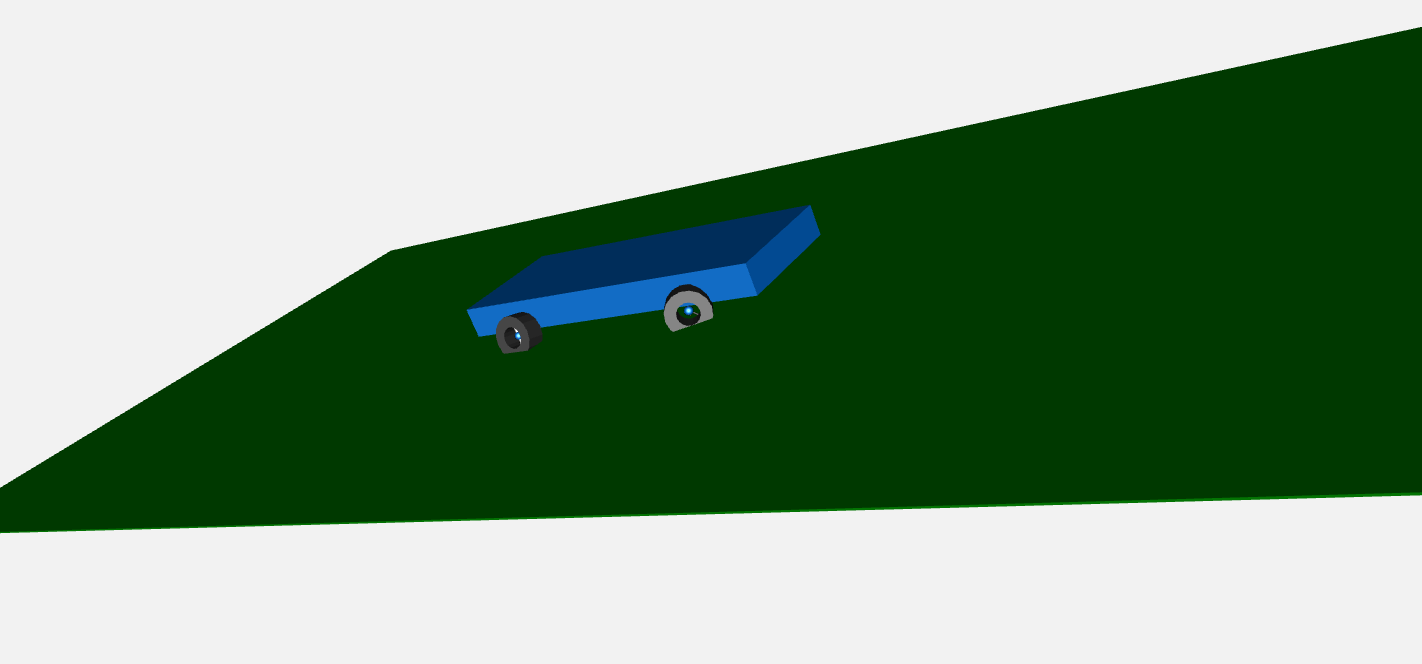
\includegraphics[width=1\textwidth]{img/bodybox.png} 
    
    \vspace{1em} % Adds spacing between image and quote
    
\caption[Representación del BodyBox en Modelica]{Representación del chasis como BodyBox dentro del visualizador de OpenModelica. Este ejemplo en particular pertenece al ejemplo \textit{E36Example} . Se puede observar un paralelepípedo al cual se le conectan las diferentes partes del sistema, como ruedas y suspensiones, y se posiciona sobre un terreno representado por $y = 1$.}
\label{fig:bodybox}
\end{figure}

\subsubsection*{Parts.Suspension}

El subpaquete \verb|Suspension| contiene los modelos que representan las diferentes geometrías de suspensión. Todos ellos extienden la clase parcial \verb|BaseSuspension|, que define la interfaz común: el conector de chasis \verb|chassisMount| (\verb|Frame_a|), el conector de rueda \verb|wheelMount| (\verb|Frame_b|), los parámetros de rigidez $k$ y amortiguamiento $d$, la masa no suspendida del buje $m_\text{hub} = 15$ kg, y el conector rotacional opcional \verb|steerInput| que se activa mediante el parámetro \verb|steerable|.\\

Se implementan tres topologías de suspensión de diferente complejidad cinemática: \verb|DoubleWishbone|, \verb|McPherson| y \verb|MultiLink|.\\

\subsubsection*{DoubleWishbone (doble triángulo).}

La suspensión de doble brazo triangular, más conocida por su nombre en inglés \verb|double wishbone|, es una de las geometrías más empleadas en vehículos de competición y alto rendimiento, tanto en el eje delantero como en el trasero. Mecánicamente, consiste en cuatro barras en el plano frontal del vehículo, cuyos eslabones son: el chasis, el brazo superior (\textit{upper A-arm}), el mangueto (\textit{knuckle}) y el brazo inferior (\textit{lower A-arm}). Cada brazo pivota en el chasis mediante una rótula o bujes de goma (modelados en Modelica como \verb|Revolute| con eje transversal $\{1,0,0\}$) y se une al mangueto en su extremo exterior mediante rótulas esféricas (los puntos de rótula superior e inferior, \textit{upper} y \textit{lower ball joints}).\\

La principal ventaja de esta topología es el control independiente de la geometría cinemática de la rueda. A diferencia de una suspensión convencional, este diseño emplea brazos de diferente longitud y con diferentes alturas de montaje en el chasis, lo que permite gestionar el cambio de caída (\textit{camber}) de la rueda durante el recorrido vertical.  El \textit{centro instantáneo de rotación} (IC) del mangueto (la intersección de las rectas que pasan por cada brazo) determina el eje alrededor del cual oscila la rueda en cada instante. Elevando el IC por encima del suelo mediante la geometría de los brazos, se obtiene una recuperación de camber que mantiene al neumático más perpendicular al suelo durante el balanceo de carrocería, maximizando el área de huella y la fuerza lateral generada en curvas rápidas.\\

En la implementación de Modelica, el bucle cinemático cerrado que forma el mecanismo de cuatro barras no puede expresarse con una cadena abierta de articulaciones y cuerpos. Para resolverlo, se utiliza el objeto \verb|JointRRR| de la biblioteca \textit{MultiBody}, que parametriza analíticamente un sistema de tres revolutes y dos barras de longitud fija. El primer revolute (\verb|frame_a|) se ubica en la rótula superior, con el brazo superior como la rama de árbol cinemático, los dos revolutos restantes, junto con sus barras asociadas, forman el cierre del bucle: la barra \verb|rRod1_ia| $= \{0, -(h_\text{sup} + h_\text{inf}), 0\}$ representa el mangueto (de longitud $h_\text{sup} + h_\text{inf} = 0{,}40$ m en la parametrización por defecto) y la barra \verb|rRod2_ib| $= \{0, 0, \pm L_\text{inf}\}$ representa el brazo inferior. Esta forma de modelar el sistema permite al compilador de OpenModelica resolver el sistema de restricciones algebraicas sin introducir multiplicaciones de Lagrange extra reduciendo el índice del DAE resultante y mejorando la estabilidad numérica \cite{otter2003}.\\

El centro de la rueda se ubica en el punto medio del mangueto, a $\frac{h_\text{sup} + h_\text{inf}}{2}$ por debajo de la rótula superior, mediante una traslación fija \verb|wheelOffset|. El amortiguador conecta un punto elevado del chasis (\verb|shockTopMount|, a 0{,}35 m sobre el montaje de la suspensión) con el punto de rótula inferior (\verb|frame_im| del \verb|JointRRR|), de manera que la fuerza del resorte actúa aproximadamente en la dirección vertical, en la región del espacio entre los dos brazos.\\

La dirección se implementa mediante un \verb|Revolute| adicional con eje vertical $\{0,1,0\}$ (eje de pivote o eje de \textit{kingpin}), interpuesto entre \verb|wheelOffset| y \verb|wheelMount|. En los ejes que permiten dirección (\verb|steerable = true|), la posición angular de este \verb|Revolute| es impuesta por el actuador \verb|steerAct|. En los ejes sin dirección, el \verb|Revolute| queda bloqueado cinemáticamente por un componente \verb|Fixed| conectado en una cláusula condicional \verb|if not steerable|, un idioma propio de Modelica que elimina físicamente el componente del sistema de ecuaciones cuando la condición no se cumple.\\

% \begin{figure}[H]
% \centering
% \begin{tikzpicture}[scale=1.25, >=Latex, font=\small,
%     piv/.style={circle, draw, fill=white, line width=0.8pt, inner sep=1.5pt},
%     bj/.style={circle, draw, fill=black, inner sep=1.5pt},
%     arm/.style={line width=1.4pt, black!75}]

%   % --- coordenadas ---
%   \coordinate (A)  at (0,2.4);      % pivote superior en el chasis
%   \coordinate (B)  at (0,1.6);      % pivote inferior en el chasis
%   \coordinate (C)  at (3.6,2.76);   % rótula superior
%   \coordinate (D)  at (4.0,0.4);    % rótula inferior
%   \coordinate (W)  at (3.8,1.58);   % centro de rueda
%   \coordinate (IC) at (-2.0,2.2);   % centro instantáneo
%   \coordinate (S)  at (0,3.2);      % anclaje superior del amortiguador
%   \coordinate (M)  at (1.6,1.12);   % anclaje inferior (sobre el brazo inferior)
%   \coordinate (P)  at (3.8,0);      % huella de contacto

%   % --- suelo ---
%   \draw[line width=1pt] (-2.6,0) -- (5.7,0);
%   \foreach \x in {-2.5,-2.2,...,5.6} \draw[black!55] (\x,0) -- ++(-0.18,-0.22);

%   % --- chasis ---
%   \fill[black!10] (-0.55,1.15) rectangle (0,3.45);
%   \draw[line width=1pt] (0,1.15) -- (0,3.45);
%   \foreach \y in {1.3,1.6,...,3.4} \draw[black!45] (-0.55,\y) -- ++(0.2,-0.18);
%   \node[anchor=south] at (-0.27,3.5) {chasis};

%   % --- construcción del centro instantáneo ---
%   \draw[dashed, black!55] (C) -- (IC);
%   \draw[dashed, black!55] (D) -- (IC);
%   \node[bj, fill=black!55, inner sep=1.3pt] at (IC) {};
%   \node[anchor=east] at (IC) {CI};

%   % --- rueda ---
%   \draw[line width=1.5pt, black!45] (W) circle (1.58);
%   \node[black!55] at (3.0,0.5) {rueda};

%   % --- muelle-amortiguador ---
%   \draw[decorate, decoration={coil, aspect=0.6, segment length=2.2mm, amplitude=1.5mm},
%         line width=0.8pt] (S) -- (M)
%         node[midway, sloped, below=1pt, font=\footnotesize]{resorte-amortiguador};

%   % --- brazos y mangueto ---
%   \draw[arm] (A) -- (C) node[midway, sloped, above=2pt]{brazo superior};
%   \draw[arm] (B) -- (D) node[midway, sloped, below=2pt]{brazo inferior};
%   \draw[arm] (C) -- (D);
%   \node[anchor=west] at (4.35,1.95) {mangueto};
%   \draw[thin] (4.33,1.95) -- (3.86,1.62);

%   % --- marcadores de articulaciones ---
%   \node[piv] at (A) {}; \node[piv] at (B) {};
%   \node[bj]  at (C) {}; \node[bj]  at (D) {};
%   \fill (W) circle (1.7pt);
%   \fill (P) circle (1.7pt); \node[anchor=north] at (3.8,-0.03) {\footnotesize huella};



% \end{tikzpicture}
\begin{figure}[htbp]
    \centering
    % Replace 'example-image' with your file name
    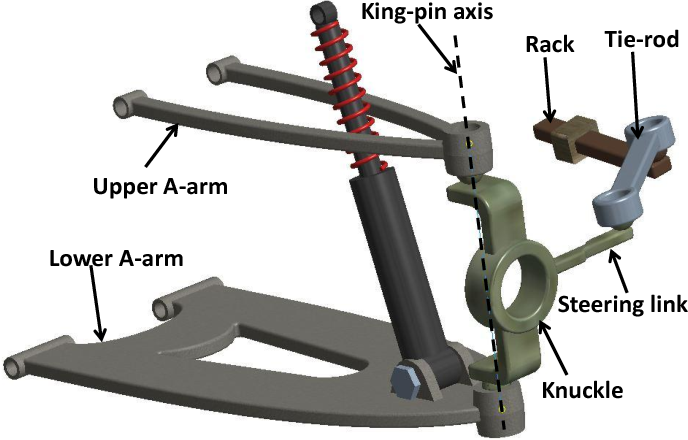
\includegraphics[width=1\textwidth]{img/double_wishbone.png} 
    
    \vspace{1em} % Adds spacing between image and quote
    

\caption[Esquema del mecanismo de doble triángulo]{Esquema cinemático de la suspensión de doble triángulo (\texttt{DoubleWishbone}) en el frontal del vehículo. El mecanismo de cuatro barras esta formado por el chasis, el brazo superior, el mangueto y el brazo inferior. El centro de la rueda se encuentra en el punto medio del mangueto. La intersección de las prolongaciones de los brazos define el centro instantáneo de rotación (IC), cuya posición controla la variación de caída durante el recorrido vertical \cite{doublewishbone}}
\label{fig:double-wishbone}
\end{figure}

\begin{figure}[htbp]
    \centering
    % Replace 'example-image' with your file name
    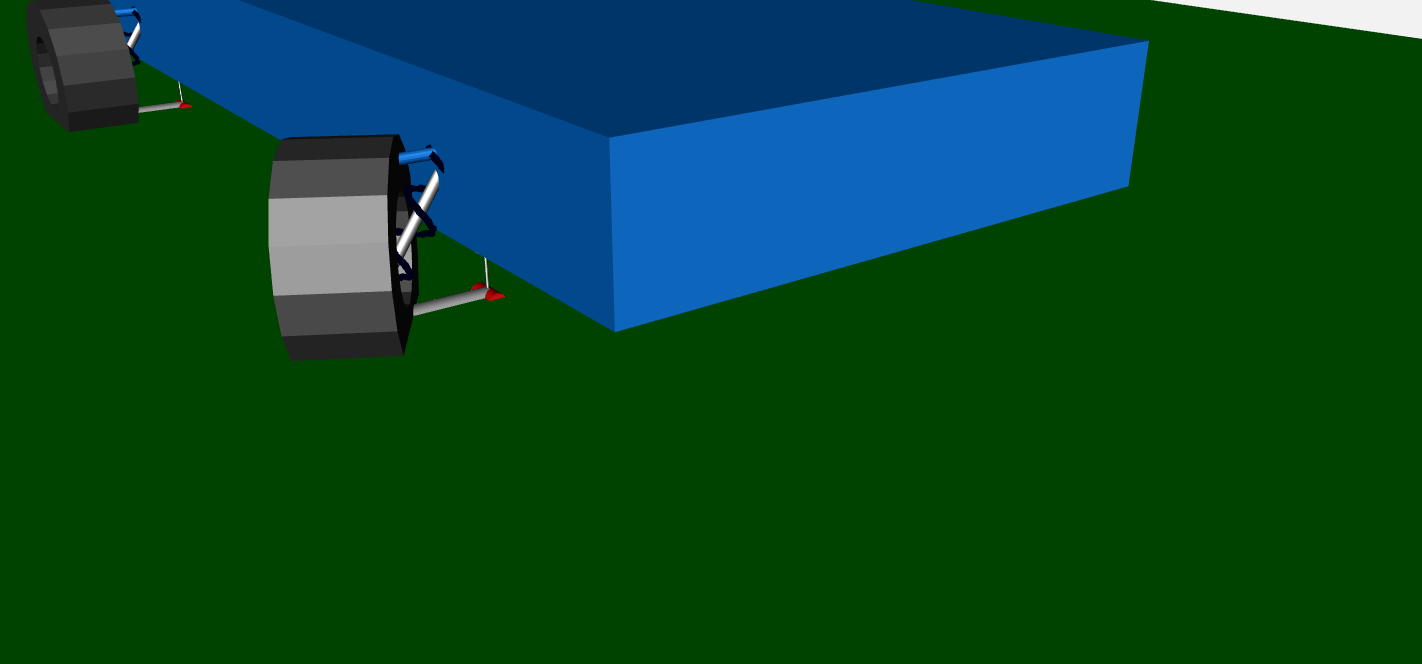
\includegraphics[width=1\textwidth]{img/doublewishbone.png} 
    
    \vspace{1em} % Adds spacing between image and quote
    
\caption[Representación de Double Wishbone en Modelica]{Representación de la geometría Double Wishbone en el visualizador de OpenModelica, con la implementación del objeto \textit{DoubleWishbone}. Esta imagen pertenece al ejemplo de \textit{CivicEKExample}, que implementa esta geometría en las cuatro puntas.}
\label{fig:doublewishbone}
\end{figure}
\newpage
\subsubsection*{McPherson (puntal telescópico).}

El puntal McPherson (\verb|McPherson Strut|) es la topología de suspensión mas utilizada en la industria automotriz de gran escala debido a su bajo coste, simplicidad constructiva y peso reducido. En un diseño real, el puntal es un elemento estructural que integra el amortiguador telescópico y la guía superior de la rueda: su extremo superior se fija a la carrocería mediante un rodamiento de apoyo que permite la rotación para la dirección, y su extremo inferior se une al mangueto (\verb|knuckle|). Un brazo inferior de triángulo (a veces conocido como parrilla) aporta la única restricción cinemática lateral, haciendo que el conjunto tenga un único grado de libertad de desplazamiento vertical. A diferencia del \verb|double wishbone|, el mangueto no tiene un punto de rótula superior independiente: el propio puntal actúa como guía rígida del mangueto, de modo que el eje de este cambia de orientación con el ángulo de dirección.\\

El modelo de esta librería, \verb|McPherson| adopta una simplificación deliberada: reemplaza el mecanismo de cinco eslabones (chasis, puntal, mangueto, brazo inferior, subchasis) por una única articulación \verb|Prismatic| de eje $\{0,-1,0\}$, que controla el desplazamiento vertical de la rueda. Esta decisión de implementación elimina el brazo inferior como restricción cinemática activa, y con ello también se pierde la variacíon de anchura de vía y de caída que aparecería en un modelo más detallado, a cambio de una mejor performance y simplicidad del modelo. Para reemplazar al brazo inferior se introduce una traslación fija \verb|knuckleOffset| que desplaza el centro de rueda respecto al extremo del puntal: \verb|wheelOffsetY| eleva el centro de rueda sobre la base del puntal (equivalente a la altura del mangueto) y \verb|wheelOffsetZ| lo desplaza lateralmente hacia el exterior (equivalente a la longitud efectiva del brazo inferior). Estos dos parámetros deben ajustarse en cada modelo de vehículo concreto para que la anchura de vía y la altura de rodaje del eje delantero sean coherentes con la geometría real del vehículo.\\

El resorte-amortiguador conecta el montaje superior fijo al chasis (\verb|shockTopMount|, elevado 0{,}28 m sobre el punto de anclaje del puntal con las configuraciones estándar) con la base del puntal (\verb|strutTravel.frame_b|). Por defecto, la longitud libre del conjunto es de 0{,}41 m, calculada geométricamente como $\sqrt{(0{,}28)^2 + (0{,}30)^2}$ para que el resorte este sin carga con el puntal a 0{,}30 m de compresión inicial. La dirección se implementa con el mismo \verb|Revolute| de eje vertical y la misma lógica condicional que en \verb|DoubleWishbone|.\\

La simplificación introducida es aceptable en el contexto de la dinámica vehicular a escala global: para la predicción del balanceo y transferencia de pesos laterales, las contribuciones de la cinemática de suspensión de primer orden son pequeñas frente a las de rigidez del resorte y la masa de la carrocería. Esta topología se emplea en el modelo \verb|E36Car| para el eje delantero, donde la limitación de espacio y la tracción trasera hacen que la variación de caída durante el giro no sea el factor limitante del comportamiento dinámico.\\

\begin{figure}[htbp]
% \centering
% \begin{tikzpicture}[scale=1.25, >=Latex, font=\small,
%     piv/.style={circle, draw, fill=white, line width=0.8pt, inner sep=1.5pt},
%     bj/.style={circle, draw, fill=black, inner sep=1.5pt},
%     arm/.style={line width=1.4pt, black!75}]

%   % --- coordenadas ---
%   \coordinate (B) at (0,0.9);       % pivote del brazo inferior en el chasis
%   \coordinate (L) at (3.1,0.55);    % rótula inferior
%   \coordinate (S) at (2.75,3.5);    % apoyo superior (cojinete a la carrocería)
%   \coordinate (Q) at (2.93,1.7);    % asiento inferior del resorte
%   \coordinate (T) at (2.95,1.55);   % unión del mangueto al puntal
%   \coordinate (W) at (3.75,1.55);   % centro de rueda
%   \coordinate (P) at (3.75,0);      % huella de contacto
%   \coordinate (G) at (3.165,0);     % eje de dirección en el suelo

%   % --- suelo ---
%   \draw[line width=1pt] (-1.4,0) -- (5.7,0);
%   \foreach \x in {-1.3,-1.0,...,5.6} \draw[black!55] (\x,0) -- ++(-0.18,-0.22);

%   % --- chasis ---
%   \fill[black!10] (-0.55,0.55) rectangle (0,2.5);
%   \draw[line width=1pt] (0,0.55) -- (0,2.5);
%   \foreach \y in {0.7,1.0,...,2.4} \draw[black!45] (-0.55,\y) -- ++(0.2,-0.18);
%   \node[anchor=south] at (-0.27,2.55) {chasis};

%   % --- eje de dirección (kingpin) hasta el suelo ---
%   \draw[dashed, black!55] (2.68,3.72) -- (G);
%   \node[anchor=east, font=\footnotesize] at (2.0,0.42) {eje de dirección};
%   \draw[thin] (2.05,0.42) -- (3.12,0.33);

%   % --- apoyo superior (cojinete a la carrocería) ---
%   \draw[line width=1pt] (2.35,3.62) -- (3.15,3.62);
%   \foreach \x in {2.4,2.6,...,3.1} \draw[black!55] (\x,3.62) -- ++(0.14,0.16);
%   \node[anchor=south, font=\footnotesize] at (2.75,3.7) {apoyo superior};

%   % --- rueda ---
%   \draw[line width=1.5pt, black!45] (W) circle (1.55);
%   \node[black!55] at (4.45,2.35) {rueda};

%   % --- puntal: resorte (coil) + vástago ---
%   \draw[decorate, decoration={coil, aspect=0.6, segment length=2.2mm, amplitude=1.6mm},
%         line width=0.8pt] (S) -- (Q);
%   \draw[arm] (Q) -- (L);
%   \node[anchor=east, align=center, font=\footnotesize] at (2.1,2.6) {puntal\\(resorte-\\amortiguador)};

%   % --- brazo inferior ---
%   \draw[arm] (B) -- (L) node[midway, sloped, below=2pt]{brazo inferior};

%   % --- mangueto / spindle ---
%   \draw[arm] (T) -- (W);
%   \node[anchor=south west, font=\footnotesize] at (3.15,1.6) {mangueto};

%   % --- marcadores de articulaciones ---
%   \node[piv] at (S) {};
%   \node[piv] at (B) {};
%   \node[bj]  at (L) {};
%   \fill (W) circle (1.7pt);
%   \fill (P) circle (1.7pt); \node[anchor=north] at (3.75,-0.03) {\footnotesize huella};

% \end{tikzpicture}
\centering
% Replace 'example-image' with your file name
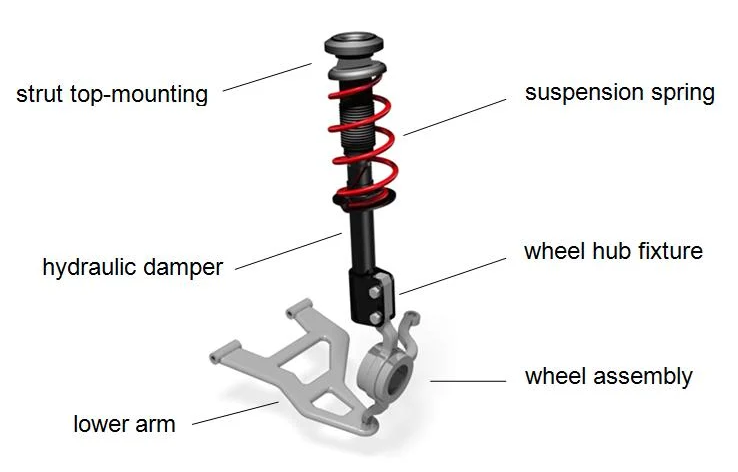
\includegraphics[width=1\textwidth]{img/mcpherson_diag.png} 

\vspace{1em} % Adds spacing between image and quote
    

\caption[Esquema del puntal McPherson]{Esquema del puntal \texttt{McPherson}. El conjunto resorte-amortiguador (puntal) es a la vez elemento elástico y guía superior de la rueda: su extremo superior se ancla a la carrocería mediante un buje que permite el giro de dirección, y su extremo inferior forma cuerpo con el mangueto. Un único brazo inferior aporta la localización lateral, con una rótula esférica  en la rueda y una articulación Revolute en el chasis. A diferencia del doble triángulo, no existe rótula superior independiente: el eje de dirección queda definido por la recta que une el apoyo superior con la rótula inferior. \cite{mchperson}}
\label{fig:mcpherson}
\end{figure}
\newpage

\subsubsection*{MultiLink (eje de vínculos múltiples).}

La suspensión multibrazo (más conocida como \textit{Multilink}) es la arquitectura de mayor complejidad cinemática de las implementadas. En un eje trasero Multilink (como el eje \textit{Z} (o \textit{Z-Axle} utilizada en el BMW E36) cada rueda está guida por cinco eslabones independientes: uno o dos brazos transversales, uno o dos brazos longitudinales y un tirante adicional \cite{reimpell2001}.  La separación de las funciones de guiado longitudinal, lateral y angular en eslabones distintos ofrece una mayor libertad de diseño comparada con otros tipos de geometría, el diseñador puede utilizar de forma casi independiente la convergencia (\textit{toe}), la caída (\textit{camber}), el avance (\textit{caster}) y la inclinación del pivote (\textit{kingpin inclination}) resultantes de cualquier combinación de desplazamiento vertical y fuerza de neumático.\\

El modelo \verb|MultiLink| implementa una versión reducida con dos eslabones transversales  (un enlace superior y un enlace inferior), conservando la topología de cuatro barras del doble triángulo pero con brazos más cortos y con el pivote del enlace inferior desplazado longitudinalmente. El cierre del bucle cinemático emplea exactamente la misma estrategia \verb|JointRRR| que \verb|DoubleWishbone|: la barra \verb|rRod1_ia| modela el mangueto y la barra \verb|rRod2_ib| modela el enlace inferior (longitud \verb|lowerLinkLength| $= 0{,}38$ m en dirección lateral).\\

% El elemento que lo diferencia de \verb|DoubleWishbone| es el parámetro \verb|rearLinkOffset|, que traslada el punto de anclaje del enlace inferior en el chasis una distancia definida (por defecto 0{,}08 m) en la dirección longitudinal $X$. Esta asimetría introduce un acoplamiento entre el desplazamiento vertical de la rueda y su ángulo de convergencia: cuando la rueda sube en compresión, el extremo interior del enlace inferior traza un arco en torno a un pivote desplazado, generando un movimiento de convergencia (\textit{toe-in}) pasivo. Este efecto (conocido como \textit{passive rear-wheel steering}) mejora la estabilidad en frenada y en la entrada a curva al aumentar la rigidez efectiva del eje ante perturbaciones laterales, sin necesitar actuadores adicionales \cite{milliken1995,reimpell2001}.  Es precisamente esta característica la que distingue al eje \textit{Z} de una simple suspensión de doble triángulo trasera.\\

% Sus dos eslabones tienen longitudes distintas, lo que genera una ganancia de caída: las dos rótulas describen arcos de radio diferente y el mangueto se va inclinando a lo largo del recorrido. Para que esa ganancia se organice alrededor de cero y no alrededor de un valor constante, el pivote del enlace inferior se sitúa más adentro que el del superior, exactamente la diferencia de longitudes (\verb|lowerLinkInboard|), con lo cual en la pose nominal ambas rótulas comparten estación lateral.\\

% La característica que lo distingue del doble triángulo, sin embargo, es la orientación del eje de articulación del varillaje. El \verb|JointRRR| obliga a que sus tres revolutos sean paralelos a un mismo eje, y el mangueto gira alrededor de ese eje a medida que la suspensión recorre. Cuando el eje es longitudinal, como en el doble triángulo, ese giro es caída y nada más. Aquí el eje está barrido un ángulo \verb|linkSweep| hacia la vertical, de $15$ grados por defecto, y el mismo giro del mangueto se reparte entonces entre caída y convergencia en la razón $\tan(\verb|linkSweep|)$. El recorrido vertical de la rueda pasa así a producir un ángulo de dirección: es la dirección pasiva de las ruedas traseras (\textit{passive rear-wheel steering}), que mejora la estabilidad en frenada y en la entrada a curva sin necesitar actuador alguno \cite{milliken1995,reimpell2001}. Se trata de la geometría de un brazo semi-arrastrado, que es de donde deriva el eje \textit{Z} del E36.\\

La característica que lo distingue del \textit{double wishbone} es la orientación del eje de articulación del varillaje. El \verb|JointRRR| fuerza a sus tres revolutes a ser paralelos y el mangueto gira alrededor de ese eje a medida de que la suspensión recorre su trayectoria. Cuando el eje es longitudinal, como en el doble triángulo, ese giro es caída y nada más. Aquí el eje está en un ángulo \verb|linkSweep| hacia la vertical, de $15$ grados por defecto y el mismo giro del mangueto se reparte entonces entre caída y convergencia. El recorrido vertical de la rueda pasa así a producir un ángulo de dirección pasiva en las ruedas traseras (\textit{passive rear-wheel steering}), que mejora la estabilidad en frenada y en la entrada a curva sin necesitar actuador alguno \cite{milliken1995,reimpell2001}. Se trata de la geometría de un brazo semi-arrastrado (\textit{semi-trailing-arm}), que es de donde deriva el eje \textit{Z} del E36. \\

El parámetro \verb|rearLinkOffset| traslada el anclaje del enlace inferior $0{,}03$ m en la dirección longitudinal $X$, de modo que el plano en el que se mueve el cuadrilátero queda inclinado hacia adelante, obteniendo $5{,}0$ grados de avance (\textit{caster}), valor representativo de un vehículo de calle.\\

Se deben aclarar las limitaciones de este modelo. En un eje multibrazo real los cinco eslabones tienen ejes de articulación no paralelos, lo que les permite prescribir convergencia, caída y avance de forma casi independiente entre sí. El objeto \verb|JointRRR| impone que los tres ejes de revolución sean paralelos, por lo que el mecanismo conserva un único grado de libertad y el reparto entre caída y convergencia queda fijado por el barrido del eje, no se pueden ajustar por separado. Esa es precisamente la limitación conocida del brazo semi-arrastrado, y no una consecuencia de la implementación.\\




% Se debe aclarar las limitaciones de este modelo: en un eje multibrazo real, los cinco eslabones tienen ejes de articulación no paralelos, lo que genera la llamada dirección pasiva de las ruedas traseras (\textit{passive rear-wheel steering}), debido al cambio dinámico del ángulo de convergencia con respecto al recorrido vertical. El ensamblaje de \verb|JointRRR| impone que los tres ejes de revolución sean paralelos entre sí, por lo que evita que el cuadrilátero pueda alterar la convergencia, que se genera con un giro del eje vertical.

% \paragraph{Lo que esta topología reducida no reproduce.} Conviene delimitar el alcance del modelo. En un eje multibrazo real —el eje \textit{Z} del BMW E36 es el caso de referencia— los cinco eslabones tienen ejes de articulación no paralelos, y es esa condición la que permite prescribir un acoplamiento entre el recorrido vertical y el ángulo de convergencia: la llamada dirección pasiva de las ruedas traseras (\textit{passive rear-wheel steering}), que mejora la estabilidad en frenada y en la entrada a curva sin requerir actuador alguno \cite{milliken1995,reimpell2001}. El ensamblaje \verb|JointRRR| impone en cambio que los tres ejes de revolución sean paralelos entre sí, lo que confina el mecanismo a un movimiento plano; y un cuadrilátero plano no puede alterar la convergencia, que es un giro alrededor del eje vertical. La medición lo verifica: la convergencia del eje trasero se mantiene en $0{,}000$ grados a lo largo de todo el recorrido. Reproducir la dirección pasiva exigiría abandonar el cierre analítico y modelar los cinco eslabones con articulaciones esféricas, a costa de introducir restricciones y variables de estado adicionales, lo que contradiría el objetivo de tiempo real que gobierna el diseño de la biblioteca. Queda por lo tanto como una simplificación asumida y no como un efecto disponible.\\


La dirección del resorte-amortiguador es análoga a la del \verb|DoubleWishbone|: desde un punto elevado del chasis (\verb|shockTopMount|, 0{,}32 m sobre el montaje) hasta el punto de rótula inferior (\verb|frame_im| del \verb|lowerLoop|). Este eje trasero no es directivo (\verb|steerable = false|), por lo que el revoluto de pivote queda bloqueado por el componente \verb|Fixed| condicional. Esto es debido a que esta geometría es utilizada en ejes traseros, por lo que normalmente no se requiere que sea direccionable.\\



\begin{figure}[htbp]
\centering
% Replace 'example-image' with your file name
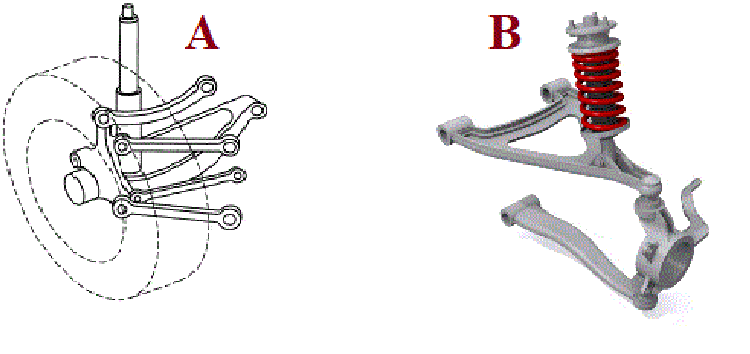
\includegraphics[width=0.8\textwidth]{img/multilink.png} 

\vspace{1em} % Adds spacing between image and quote
    

\caption[Esquema del eje MultiLink]{Esquema del eje \texttt{MultiLink}, que resalta su diferencia con respecto al doble triángulo. Los pivotes interiores del enlace superior e inferior están separados longitudinalmente una distancia \texttt{rearLinkOffset}. Esta asimetría hace que, al comprimirse la suspensión, el extremo exterior del enlace inferior describa un arco en torno a un pivote desplazado en el eje de avance, girando ligeramente el mangueto y produciendo una convergencia (\textit{toe-in}) pasiva de la rueda.\cite{multilink}}
\label{fig:multilink}
\end{figure}

\newpage

\begin{figure}[htbp]
\centering
% Replace 'example-image' with your file name
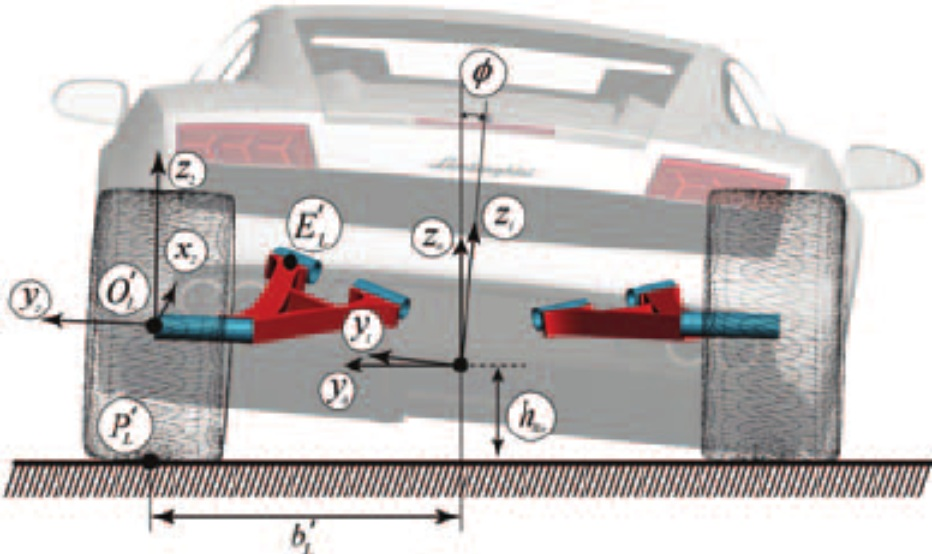
\includegraphics[width=1\textwidth]{img/trailing.jpg} 

\vspace{1em} % Adds spacing between image and quote
    

\caption[Esquema del eje MultiLink]{Esquema de la geometría \texttt{Semi-trailing-arm}, que es más cercana a la abstracción aplicada del modelo \textit{Multilink}. Se pueden apreciar como tanto la caída como la convergencia están enlazados por el mismo movimiento del recorrido de la suspensión.\cite{trailing}}
\label{fig:trailing}
\end{figure}
\newpage
\subsubsection*{Parts.RollResistance}

El subpaquete \verb|RollResistance| reúne los elementos que ayudan a la resistencia del balanceo de la carrocería. Estos elementos no afectan en el movimiento vertical del sistema. Se creó un único modelo, \verb|AntiRollBar|, que representa la barra estabilizadora en un eje.\\

Una barra estabilizadora es una barra de torsión que vincula las dos ruedas de un mismo eje. Cuando ambas ruedas recorren la misma distancia vertical, la barra gira como un cuerpo rígido, no se retuerce y no aporta rigidez, sin embargo, cuando una rueda sube y la otra baja (como por ejemplo al doblar) la barra se retuerce y aplica un par opuesto al movimiento realizado. Esto hace que se puedan montar resortes más blandos sin que el vehículo vuelque demasiado en curva.

% \paragraph{Fundamento.} Una barra estabilizadora es una barra de torsión que vincula las dos ruedas de un mismo eje a través del chasis. Cuando ambas ruedas recorren lo mismo —al pasar sobre un badén, por ejemplo— la barra gira como un cuerpo rígido, no se retuerce y no aporta rigidez alguna. Cuando en cambio una rueda sube y la otra baja, como ocurre al virar, la barra se retuerce y opone un par al movimiento diferencial. Esa selectividad es lo que la hace útil: permite montar resortes blandos, que dan una respuesta vertical cómoda, sin que el vehículo se incline en exceso en curva. Un automóvil de calle obtiene de ella una parte sustancial de su rigidez al balanceo \cite{gillespie1992}.\\

El modelo expone cuatro conectores \verb|Frame_a|: el anclaje al chasis y el montaje de rueda de cada lado. Dos sensores \verb|RelativePosition| miden la altura del centro de rueda respecto de su anclaje y el se aplica una fuerza que responde a la diferencia entre ambas alturas:

% \paragraph{Implementación.} El modelo expone cuatro conectores \verb|Frame_a|: el anclaje al chasis y el montaje de rueda de cada lado. Dos sensores \verb|RelativePosition| miden la altura de cada centro de rueda respecto de su propio anclaje, resuelta en ejes del chasis para que la referencia siga a la carrocería cuando esta balancea, y el elemento responde a la diferencia entre ambas:

\begin{equation}
    f = c_\text{arb} \cdot \frac{d_\text{izq} - d_\text{der}}{2}
    \label{eq:arb}
\end{equation}

La fuerza resultante se aplica utilizando dos elementos \verb|Forces.Force| que conectan en cada lado el anclaje al chasis y el montaje de la rueda. Se aplica una fuerza hacia abajo en la rueda más comprimida (y hacia arriba en el chasis de esa esquina) y otra opuesta en la otra rueda. \\

% La fuerza resultante se aplica hacia abajo en la rueda más comprimida y hacia arriba en la otra, mediante dos elementos \verb|Forces.Force| que abarcan, en cada lado, el anclaje al chasis y el montaje de rueda. Recurrir a un elemento de fuerza de \textit{MultiBody} en lugar de aplicar el par de fuerzas directamente sobre las ruedas no es una cuestión de estilo: el elemento reparte por sí mismo la reacción sobre el marco de origen, con lo cual el conjunto queda en equilibrio. Aplicar únicamente las dos fuerzas sobre las ruedas dejaría sobre el vehículo un par de balanceo externo sin reacción, que le haría ganar cantidad de movimiento angular sin causa física.\\

% \paragraph{Propiedades.} En recorrido simétrico la diferencia de la Ecuación~\ref{eq:arb} se anula y la barra no interviene en absoluto, de modo que las frecuencias verticales del vehículo quedan intactas y su efecto se limita al balanceo. La ley es además puramente algebraica, por lo que el elemento agrega ecuaciones pero no estados continuos y no incrementa el tamaño del vector que el integrador debe resolver, consideración que pesa en un modelo destinado a ejecutarse en tiempo real. El parámetro \verb|c_arb| expresa la rigidez de la barra referida a la rueda, en N/m; su valor por defecto es nulo, lo que la deja inactiva.\\

Los tres vehículos fueron equipados con barras en ambos ejes. El monoplaza lleva $13$ kN/m en cada uno, el E36, $31$ kN/m adelante y $16$ kN/m atrás, el Civic, $41$ y $23$ kN/m. En los dos vehículos de calle el reparto es delantero, disposición habitual para favorecer el subviraje en el límite, lo que lleva a una mayor seguridad en el manejo.\\


\subsubsection*{Parts.Tires}

El subpaquete \verb|Tires| se encarga de modelar los neumáticos como cuerpos rígidos con masa $m_\text{tire} = 20$ kg (por defecto) conectados a la suspensión mediante un \verb|Revolute| de giro libre, se implementaron dos variantes:

\begin{itemize}
    
    \item \verb|Tire|: Neumático pasivo. El \verb|Revolute| que se encarga del giro tiene su brida de eje expuesta como \verb|brakeFlange| (\verb|flange_b|) para la conexión del freno, pero no recibe par motor, representa una rueda no traccionada.
    
    \item \verb|DrivingTire|: Neumático motriz. El modelo es idéntico a \verb|Tire|, pero añade un conector \verb|spinInput| (\verb|Flange_a|) que recibe el par de torque del diferencial. La brida de freno (\verb|brakeFlange|) y la de tracción (\verb|spinInput|) se comparten sobre el mismo eje del \verb|Revolute|, de modo que el par neto aplicado es la suma algebraica de ambas contribuciones.
\end{itemize}

El subcomponente \verb|TireVisualizer| renderiza cada neumático, copiando el objeto de la librería \textit{Visualizers} de \textit{MultiBody} \verb|MultiBody.Visualizers.VoluminousWheel|, esta se encarga de generar un toroide para la forma del neumático en sí y un cilindro hueco que representa la llanta, ambos parametrizados con el radio \verb|rTire| propagado desde el nivel de ejemplo mediante \texttt{outer}. El único cambio que se le aplicó a la clase original fueron cambios de coordenadas y orientaciones para que sigan un recorrido fiel al modelo que se está simulando.\\

\begin{figure}[htbp]
    \centering
    % Replace 'example-image' with your file name
    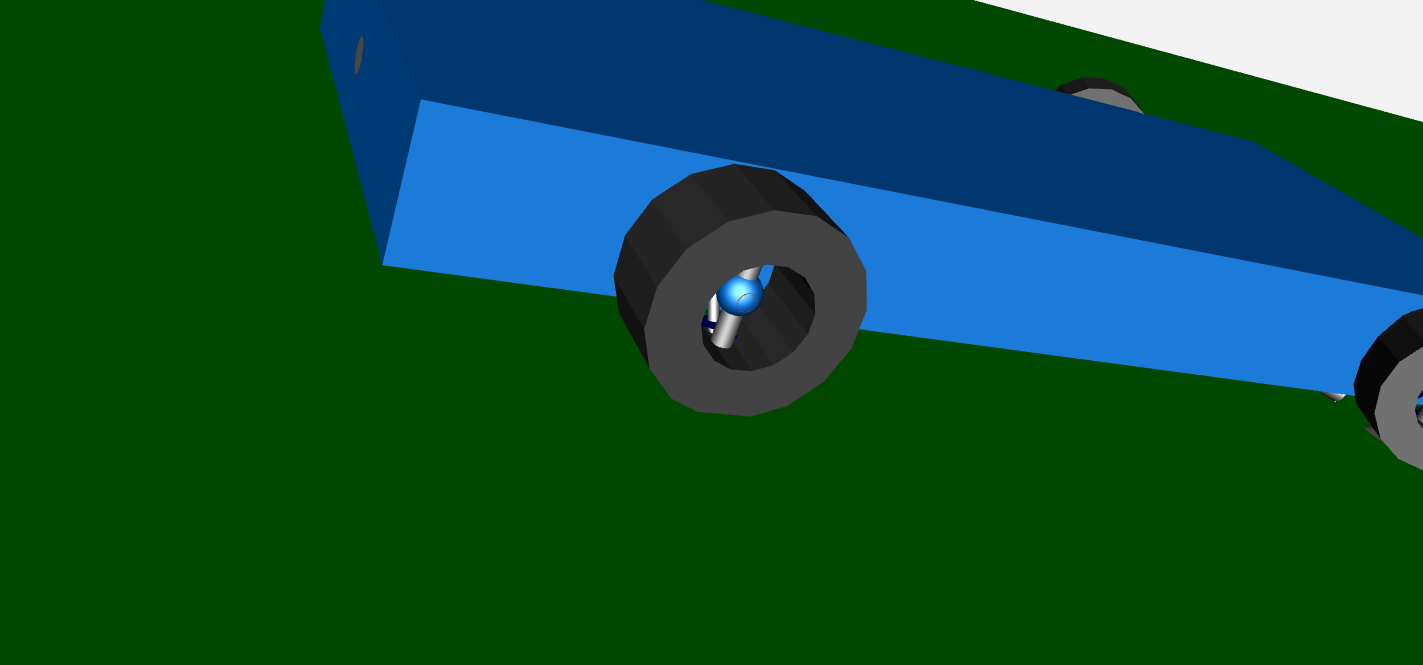
\includegraphics[width=1\textwidth]{img/tire.png} 
    
    \vspace{1em} % Adds spacing between image and quote
    
\caption[Representación de Tire en Modelica]{Representación de una rueda utilizando el objeto \textit{Tire} dentro del visualizador de OpenModelica, la geometría es generada por el componente \textit{TireVisualizer}. Esta imágen fue capturada del ejemplo \textit{CivicEKExample}, la rueda está conectada al chasis mediante una geometría de suspensión Double Wishbone}
\label{fig:tire}
\end{figure}

\subsubsection*{Parts.Differentials}

El subpaquete \verb|Differentials| modela el componente que se encarga de transmitir el par proveniente de la transmisión a las ruedas. La clase parcial \verb|Differential| define únicamente la interfaz mecánica común: una brida rotacional de entrada de par \verb|pedalInput| (\verb|Flange_a|), alimentada por la transmisión, y dos bridas rotacionales de salida hacia las ruedas (\verb|left_out| y \verb|right_out|). No contiene ecuaciones, ya que es cada subclase concreta la que decide cómo el par se distribuye en las dos ruedas.\\

\subsubsection*{Eje rígido}

Un eje rígido (\textit{solid axle} o \textit{live axle}) conecta mecánicamente ambas ruedas del mismo eje mediante semiejes que giran necesariamente a la misma velocidad angular. Esta arquitectura es la más sencilla posible desde el punto de vista constructivo, tiene consecuencias directas en el comportamiento en la curva, al doblar, la rueda exterior debe recorrer un arco de mayor radio que la interior y, por lo tanto debería girar más rápido, pero, al estar ambas ruedas girando a la misma velocidad, esta diferencia de velocidad se absorbe mediante deslizamiento lateral de los neumáticos (\textit{tire scrub}), lo que genera calor, desgaste y una tendencia al sobreviraje en curvas cerradas. En lo que respecta a la dinámica del vehículo, el eje rígido introduce un acoplamiento entre el movimiento de guiñada (\textit{yaw}) del chasis y el estado de tracción de ambas ruedas: en una curva cerrada con aceleración, la rueda interior tiende a patinar antes que la exterior, ya que recibe el mismo par pero con menor carga, comportamiento característico del vehículo de tracción trasera con eje sólido. Este tipo de eje es muy común en kartings debido a su simplicidad de mantenimiento. \\

\paragraph{Implementación como nodo mecánico de par.}

A diferencia de un enfoque basado en una restricción cinemática de velocidad, que forzaría ambas ruedas a igual velocidad, pero que introduciría un lazo algebraico de índice elevado e impediría que el par de frenado modificara la velocidad de las ruedas motrices, \verb|SolidAxle| se implementa como un simple nodo mecánico: conecta la brida de entrada \verb|pedalInput| directamente a ambas salidas \verb|left_out| y \verb|right_out|, de modo que la transmisión y las dos ruedas comparten un único nodo rotacional:

\begin{equation}
    \varphi_\text{ped} = \varphi_\text{izq} = \varphi_\text{der}
\end{equation}

Ambas ruedas traseras giran a la misma velocidad angular, sin acción diferencial de velocidad, como corresponde a un eje bloqueado, y el par entregado por la transmisión se distribuye mecanicamente a través de ese nodo hacia las ruedas, en vez de ser forzado por una fuente interna. El modelo no tiene parámetros propios: el esfuerzo motor se fija en la transmisión (parámetro \verb|torqueValue| de \verb|MockTransmission|).\\

La ventaja de modelar el diferencial mediante intercambio de par radica en la interacción entre este y el freno. Como todos los conectores son bridas rotacionales (\verb|Flange|), cualquier par aplicado sobre las bridas de las ruedas se suma sobre el nodo compartido, de manera que el par aplicado por un objeto \verb|DiscBrake| sobre una rueda se resta directamente del par motor y desacelera el eje, como lo haría un freno real, sin necesidad de vencer ninguna restricción cinemática. La velocidad resultante de las ruedas no se impone, si no que emerge naturalmente del par motor, el de frenado, la inerciad e las ruedas y las fuerzas de contacto con el suelo. Esta clase se podría extender agregando un diferencial abierto o uno autoblocante encaminando el par de entrada a través de un \verb|IdealPlanetary| o de ecuaciones de reparto de par que permitan una diferencia de velocidad entre las dos ruedas.\\

\subsubsection*{Parts.Brakes}

El modelo \verb|DiscBrake| modela el comportamiento de un freno de disco, aplicando par a la brida rotacional de cada neumático.\\

\subsubsection*{DiscBrake}

En un freno a disco real, una pinza hidráulica aprieta dos pastillas de fricción contra ambas caras de un disco conectado al eje de la rueda. La fuerza de contacto normal $N$ es proporcional a la presión hidráulica del circuito de frenos, que a su vez es función de la fuerza ejercida por el conductor sobre el pedal. El par de frenado resultante sigue el modelo de fricción de Coulomb es proporcional a la fuerza normal y al coeficiente de fricción de las pastillas $\mu_p$, y actúa siempre en sentido opuesto a la rotación de la rueda \cite{rajamani2012}:

\begin{equation}
    \tau_\text{Coulomb} = -\mu_p \cdot N_{max} \cdot r_\text{eff} \cdot \text{sign}(\omega)
\end{equation}

donde $r_\text{eff}$ es el radio efectivo medio del disco. En el modelo \verb|DiscBrake|, el producto $\mu_p \cdot N_\text{max} \cdot r_\text{eff}$ queda parametrizado directamente como \verb|maxBrakeTorque| $= \tau_\text{max}$, y la demanda normalizada $u \in [0, 1]$ escala la fuerza normal, reproduciendo la relación entre la posición del pedal y el par generado:

\begin{equation}
    \tau_\text{ideal} = -u \cdot \tau_\text{max} \cdot \text{sign}(\omega)
\end{equation}

Los valores de \verb|maxBrakeTorque| asignados a los distintos vehículos de la biblioteca —2000 N$\cdot$m para el modelo genérico, 2500 N$\cdot$m en el eje delantero del E36 y 3000 N$\cdot$m en el trasero, son coherentes con los rangos de par de frenado de vehículos de turismo de producción \cite{rajamani2012}.\\

% \paragraph{El problema de la discontinuidad y la regularización \textit{tanh}.}

La función $\text{sign}(\omega)$  presenta una discontinuidad en $\omega = 0$ que tiene consecuencias graves para la integración numérica: en los solucionadores DAE de paso variable, toda discontinuidad activa un mecanismo de detección de cruce por cero (\textit{zero-crossing detection}) que obliga a reducir el paso de integración y relanzar el solver desde el instante del evento \cite{armstrong1994}. En un modelo de vehículo con cuatro frenos activos, esto puede disparar eventos múltiples y sincronizados que afectan de manera significativamente negativa al rendimiento en tiempo real. Adicionalmente, cuando la velocidad angular oscila en torno a cero (rueda próxima a bloqueo), la función signo puede provocar alternancia rápida de signo del par (chattering) que excita modos de alta frecuencia numéricamente.\\

Para resolver este problema, el modelo reemplaza la función signo por una tangente hiperbólica regularizada:

\begin{equation}
    \tau_\text{freno} = -u \cdot \tau_\text{max} \cdot \tanh\!\left(k_s \cdot \omega\right)
\end{equation}

La función $\tanh(k_s \cdot \omega)$ es $C^\infty$ en todo $\mathbb{R}$ y reproduce el comportamiento de Coulomb fuera de la zona de transición. Para analizarla, se distinguen dos regímenes según el valor de $k_s \cdot |\omega|$:

\begin{itemize}
    \item \textbf{Régimen lineal} ($k_s \cdot |\omega| \ll 1$): $\tanh(k_s\omega) \approx k_s\omega$, de modo que el freno se comporta como un amortiguador viscoso de coeficiente efectivo $u \cdot \tau_\text{max} \cdot k_s$. En este régimen, el par es proporcional a la velocidad y el sistema no tiene discontinuidades.
    \item \textbf{Régimen de Coulomb} ($k_s \cdot |\omega| \gg 1$): $\tanh(k_s\omega) \approx \pm 1$, y el freno se aproxima al modelo ideal de Coulomb con par constante $\pm u \cdot \tau_\text{max}$.
\end{itemize}

La transición entre ambos regímenes ocurre en la zona $|\omega| \approx 1/k_s$. Con $k_s = 10$ rad$^{-1}{\cdot}$s, esta zona tiene un ancho de $\pm 0{,}1$ rad/s, equivalente a aproximadamente $\pm 1$ rpm para una rueda típica. A velocidades superiores a este umbral, el freno se comporta esencialmente como el modelo de Coulomb ideal, por debajo de él, la transición suave evita cualquier evento de cruce por cero y garantiza la continuidad diferenciable del sistema \cite{armstrong1994}. Este compromiso es adecuado para la simulación de dinámica vehicular, donde el bloqueo total de una rueda es un fenómeno de interés pero la oscilación subsecuente en torno a $\omega = 0$ no lo es.\\

\subsubsection*{Parts.Transmission}


El subpaquete \verb|Transmission| abstrae la generación del par motor hacia el diferencial a partir del input de acelerador del conductor. Sigue el mismo patrón de clase parcial que el resto de la biblioteca: \verb|BaseTransmission| define la interfaz común de una entrada \verb|pedalInput| (\verb|RealInput|) con el valor normalizado del acelerador y una salida rotacional \verb|torqueOut| (\verb|Flange_a|) que entrega el par mecánico, de modo que cualquier implementación puede sustituirse sin modificar los componentes que interactúan con este objeto (diferencial, interfaz de acelerador). Este objeto ahora mismo actúa como una combinación de motor y transmisión, así que una implementación verdadera debería modelar ambos componentes.\\

Como se mencionó anteriormente, la implementación concreta \verb|MockTransmission| es una simplificación de un conjunto de motor-transmisión, que convierte el comando del pedal en par mediante una relación lineal directa:

\begin{equation}
    \tau_\text{motor} = k_\tau \cdot u_\text{pedal}
\end{equation}

donde $k_\tau$ (representado como el parámetro \verb|torqueValue|) es el par entregado a las ruedas cuando el acelerador está a fondo y  $u_\text{pedal} \in [0, 1]$ es el input normalizado. \\ 
El par se aplica a través de una fuente \verb|Modelica.Mechanics.Rotational.Sources.Torque| y fluye por una brida \verb|torqueOut| hacia el diferencial. Para simplificar, en esta implementación, el par es constante, no tiene una retroalimentación de velocidad, por lo que el vehículo acelera hasta que la tracción y las resistencias al avance lo equilibran. Al exponer una brida portadora de par, un modelo de motor realista, con mapa de par en función del régimen, inercia del volante de inercia y relaciones de cambio, puede reemplazar a \verb|MockTransmission| conservando la misma interfaz de \verb|BaseTransmission|.\\


\subsubsection*{Parts.Steering}

De la misma forma que el paquete anterior, \verb|Steering| abstrae la conversión del comando de volante en un ángulo de giro en las ruedas. La clase parcial \verb|BaseSteering| define la interfaz como una entrada \verb|steerCmd| (\verb|RealInput|) con el comando normalizado en $[-1, 1]$ y una salida \verb|steerAngle| (\verb|RealOutput|) con el ángulo de rueda resultante, en radianes.\\

La implementación \verb|MockSteering| aplica un mapeo lineal entre ambos:

\begin{equation}
    \delta = \delta_\text{max} \cdot u_\text{steer}
\end{equation}

donde $\delta_\text{max}$ (representado por el parámetro \verb|maxSteerAngle|, con valor por defecto $0{,}53$ rad $\approx 30°$) es el ángulo de rueda cuando el volante esta al máximo de su giro y $u_\text{steer} = 0$ corresponde a la marcha recta. La salida \verb|steerAngle| se conecta a los actuadores de posición (\verb|Rotational.Sources.Position|) de las dos ruedas delanteras que reciben el mismo ángulo, ya que no se está modelando la dinámica de la columna de dirección, la relación de dirección variable ni la geometría de Ackermann. Como en el caso de la transmisión, la separación de la interfaz permite sustituir \verb|MockSteering| por un modelo más detallado sin alterar el resto del vehículo.\\

\subsection{Examples}

El paquete\verb|Examples| compila los modelos ejecutables de alto nivel: los puntos de entrada de la simulación que ensamblan un vehículo completo, el entorno y los comandos del conductor en un sistema autocontenido y simulable. Cumplen una doble función, como escenarios de validación del comportamiento dinámico y como plantillas a partir de las cuales construir nuevas simulaciones.\\


Todos los ejemplos comparten la misma estructura de ensamblaje. En primer lugar, declaran el radio de rueda como un parámetro global \\ \verb|inner parameter Real R_wheel|, que se propaga por el mecanismo \texttt{inner}/\texttt{outer} a los neumáticos y a los modelos de contacto con el suelo. A continuación instancian tres bloques principales: un vehículo (\verb|Car|, \verb|CivicEKCar| o \verb|E36Car|), el entorno \verb|Roads.Road|, que a su vez posee el \verb|World|, el terreno y los cuatro contactos de rueda, y un conjunto de fuentes de señal que emulan las acciones del conductor. Estas fuentes se conectan a las entradas normalizadas \verb|throttleInput|, \verb|steerInput| y \verb|brakeInput| del vehículo, mientras que los cuatro conectores \verb|frame_FL/FR/RL/RR| del vehículo se acoplan a los del entorno, cerrando el contacto rueda-suelo.\\

La biblioteca incluye cuatro ejemplos:

\begin{center}
\begin{tabular}{llll}
\hline
\textbf{Ejemplo} & \textbf{Vehículo} & \textbf{$R$ (m)} & \textbf{Entradas del conductor} \\
\hline
\verb|CarExample|    & \verb|Car| (Formula Ford)   & 0{,}25 & acelerador y dirección constantes,\\ & & & freno escalón en $t=3$ s \\
\verb|CivicEKExample| & \verb|CivicEKCar| (Civic EK) & 0{,}30 & acelerador y dirección constantes,\\ & & & freno escalón en $t=5$ s \\
\verb|E36Example|     & \verb|E36Car| (BMW E36)      & 0{,}31 & acelerador y dirección constantes,\\& & & freno escalón en $t=5$ s \\
\verb|CarExampleUDP|  & \verb|Car|                  & 0{,}25 & acelerador constante,\\& & & dirección sinusoidal, sin freno \\
\hline
\end{tabular}
\end{center}

Los tres primeros (\verb|CarExample|, \verb|CivicEKExample| y \verb|E36Example|) son escenarios de validación de lazo abierto, ya que aplican un input de acelerador constante y un ángulo de dirección fijo sobre un terreno plano, con una aplicación de freno luego de un tiempo determinado que permite ver la transferencia de carga longitudinal y la desaceleración del tren motriz. Se diferencian en el modelo de vehículo que se instancia, cada uno parametrizado a partir de automóviles reales de arquitectura distinta:

\begin{itemize}
    
    \item \verb|CarExample| simula el modelo \verb|Car|, inspirado levemente en un monoplaza ligero tipo Formula Ford 1600. Es el más liviano y de geometría más simétrica: chasis de 400 kg con dimensiones $3{,}0 \times 1{,}8 \times 0{,}5$ m, batalla de 3{,}0 m y vía de 1{,}8 m. Utiliza suspensión \verb|DoubleWishbone| en las cuatro puntas, con la rigidez y amortiguamiento por defecto de \verb|BaseSuspension| ($k = 30$ kN/m, $d = 2500$ N$\cdot$s/m). Es un vehículo de tracción trasera, con neumáticos \verb|DrivingTire| detrás y \verb|Tire| pasivos delante, de radio $R = 0{,}25$ m. El chasis arranca suspendido a 1{,}2 m sobre el terreno y cae hasta el equilibrio estático.
    \newpage
\begin{figure}[htbp]
    \centering
    % Replace 'example-image' with your file name
    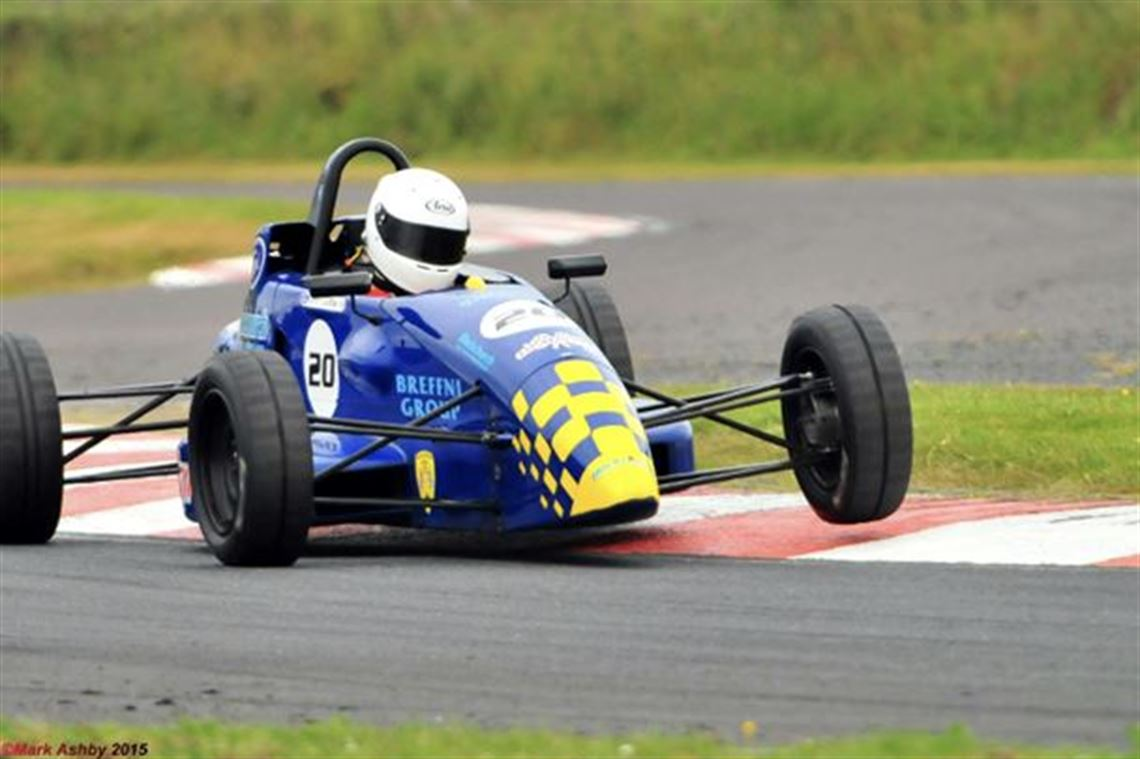
\includegraphics[width=1\textwidth]{img/fford.jpg} 
    
    \vspace{1em} % Adds spacing between image and quote
    
\caption[Formula Ford 1600]{Imágen de un vehículo Formula Ford 1600. Se puede observar las geometría de suspensión \textit{Double Wishbone}. Fuente: https://racecarsdirect.com/Advert/Details/91965/o5-ray-formula-ford-1600.}
\label{fig:ff1600}
\end{figure}

    \item \verb|CivicEKExample| simula el \verb|CivicEKCar|, basado en un Honda Civic EK hatchback de tracción delantera. Chasis de 990 kg de peso y dimensiones $4{,}178 \times 1{,}704 \times 0{,}4$ m, con batalla de 2{,}62 m y vía de 1{,}47 m. Emplea \verb|DoubleWishbone| en las cuatro esquinas, con rigidez diferenciada por eje, 16 kN/m delante y 14 kN/m detrás, y amortiguamiento de 1800 N$\cdot$s/m en las cuatro ruedas. La tracción es delantera (\verb|DrivingTire| en el eje delantero, \verb|Tire| pasivos detrás) y los neumáticos son 185/65R14 ($R = 0{,}30$ m).
\newpage
\begin{figure}[htbp]
    \centering
    % Replace 'example-image' with your file name
    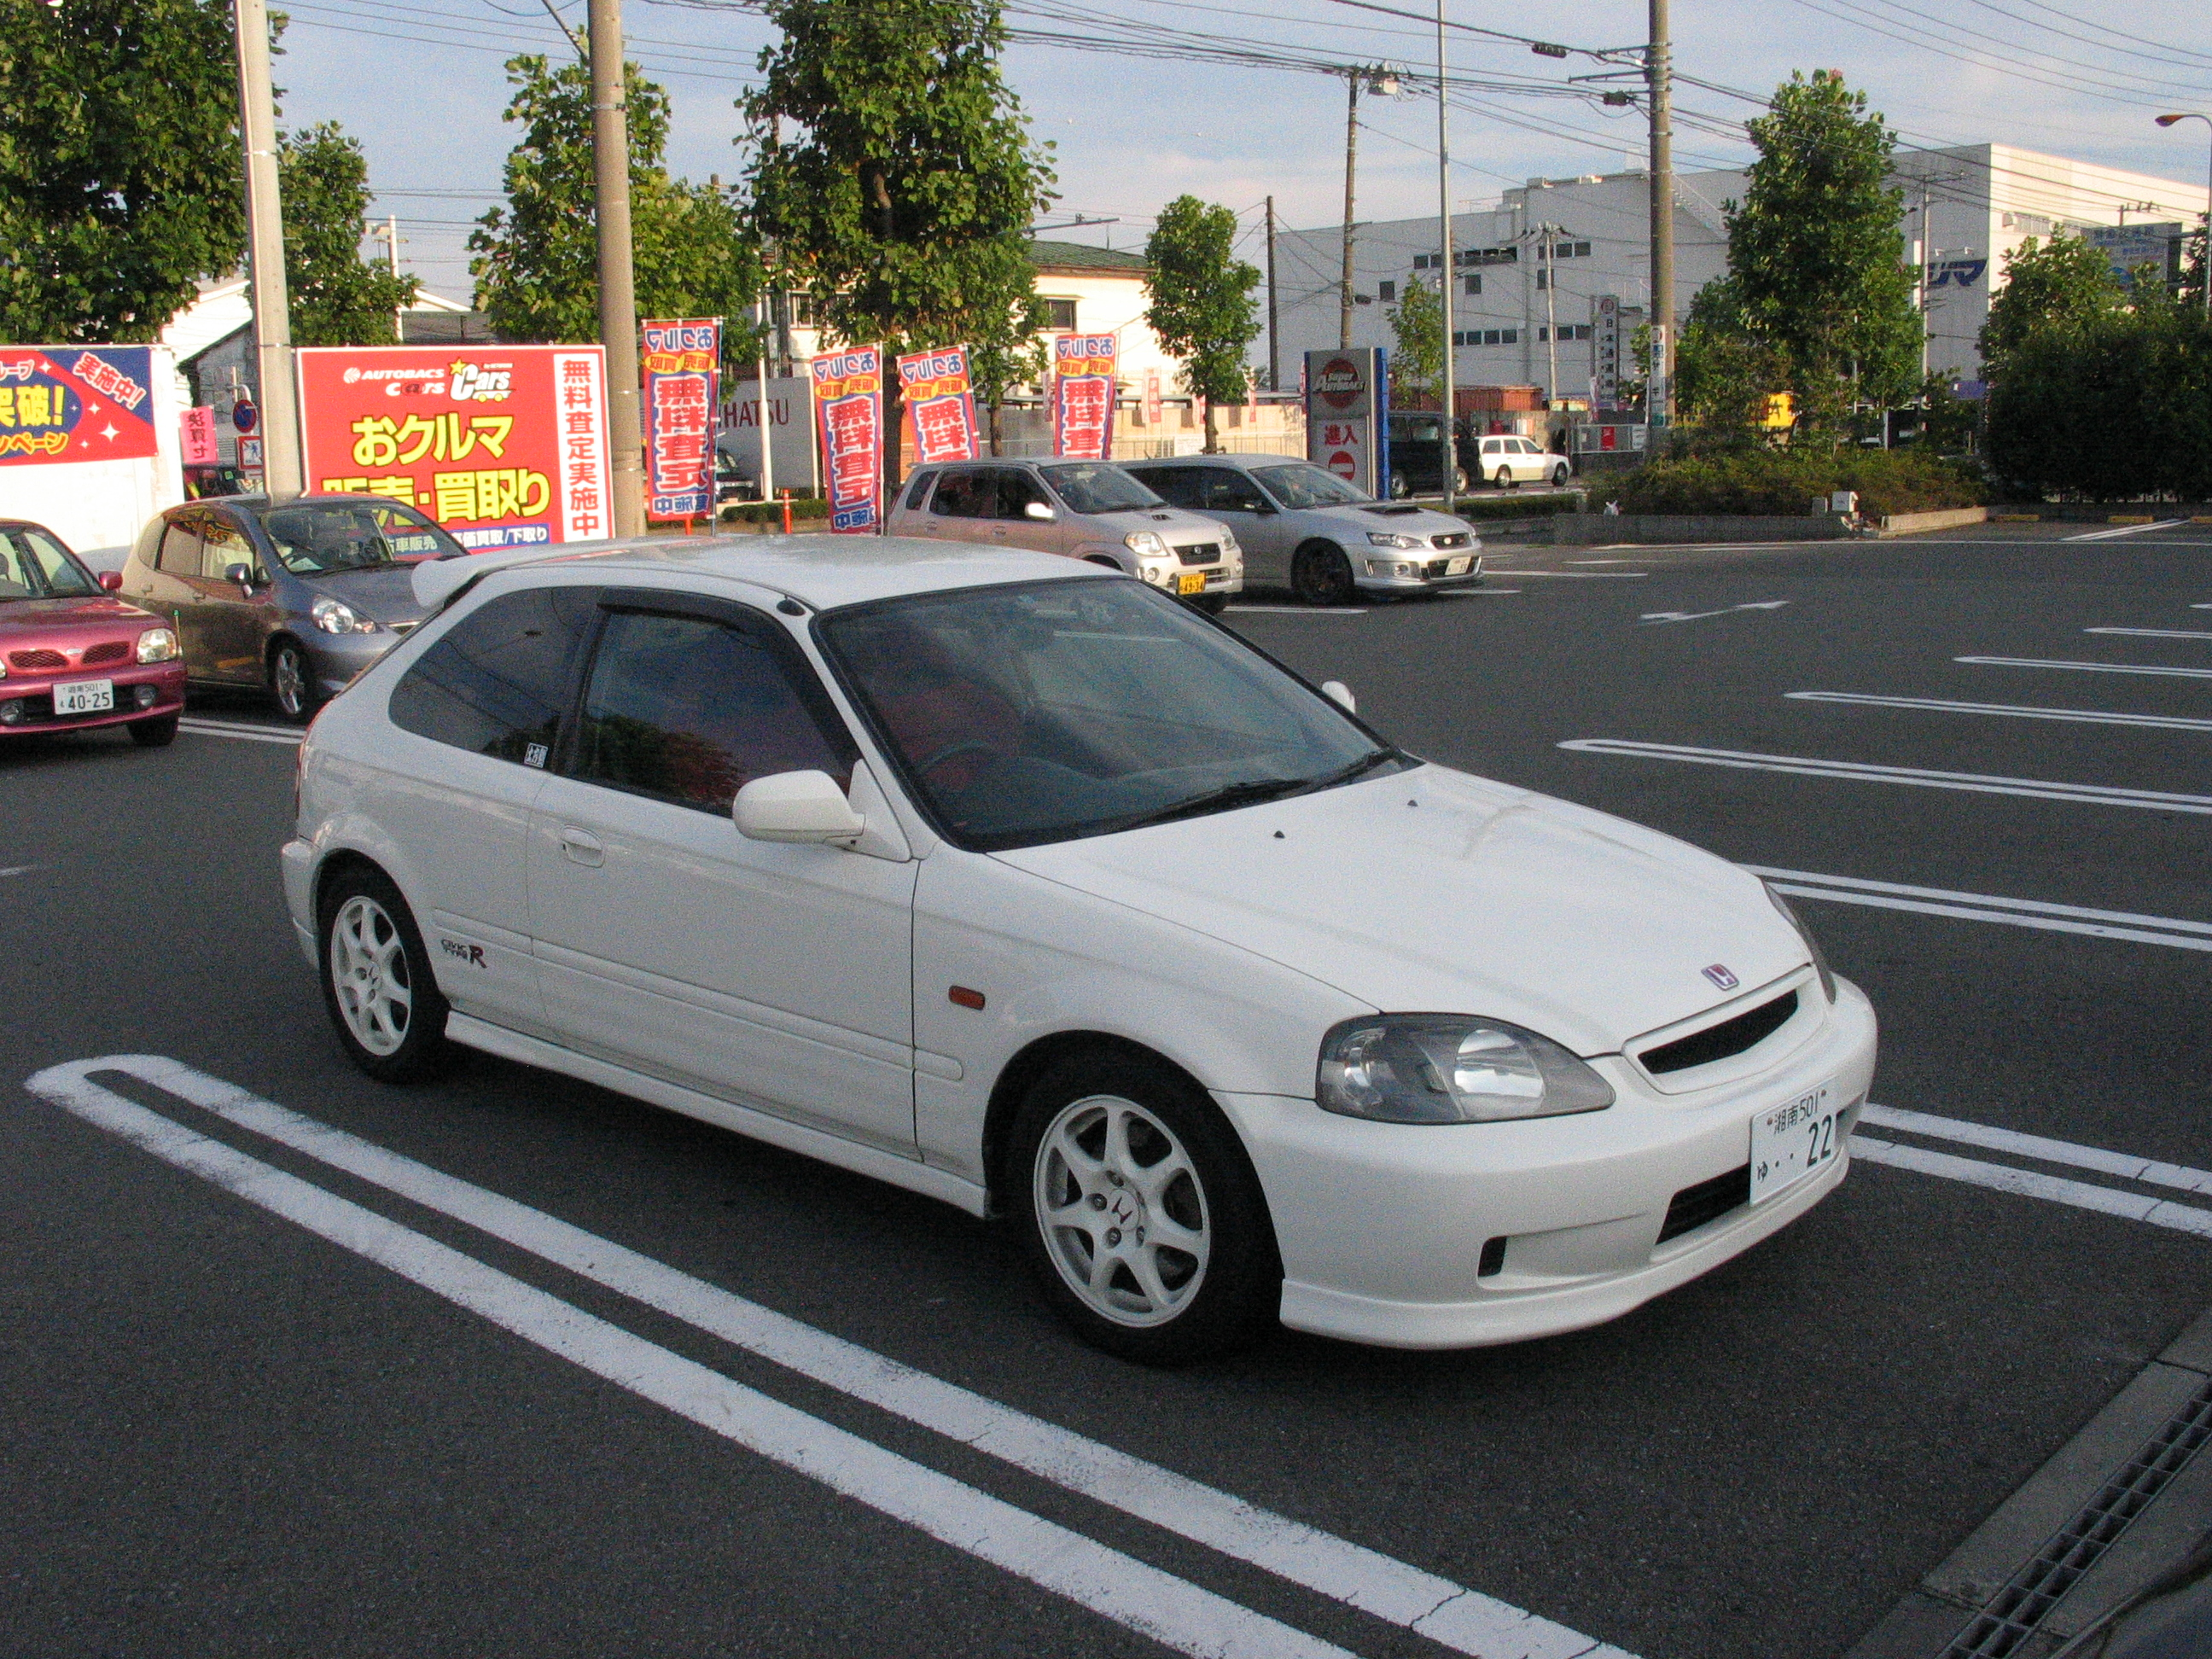
\includegraphics[width=1\textwidth]{img/civicek.jpg} 
    
    \vspace{1em} % Adds spacing between image and quote
    
\caption[Honda Civic EK]{Imágen de un vehículo Honda Civic de la generación EK. Fuente: https://es.wikipedia.org/wiki/Honda\_Civic\_(sexta\_generación).}
\label{fig:civicek}
\end{figure}
    
    \item \verb|E36Example| simula el \verb|E36Car|, basado en un BMW E36 de tracción trasera. Chasis de 1000 kg de masa suspendida y dimensiones $4{,}433 \times 1{,}710 \times 0{,}4$ m, con batalla de 2{,}70 m y vía de 1{,}42 m. Es el vehículo de geometría de suspensión más elaborada: puntal \verb|McPherson| en el eje delantero (20 kN/m, 2200 N$\cdot$s/m, con desplazamientos de mangueto \verb|wheelOffsetY| $= 0{,}25$ m y \verb|wheelOffsetZ| $= 0{,}30$ m para restituir la vía y la altura del centro de rueda) y eje trasero \verb|MultiLink| de tipo Z (16 kN/m, 2200 N$\cdot$s/m), con \verb|DrivingTire| en el eje trasero. Los neumáticos son 195/65R15 ($R = 0{,}31$ m).
\newpage
\begin{figure}[htbp]
    \centering
    % Replace 'example-image' with your file name
    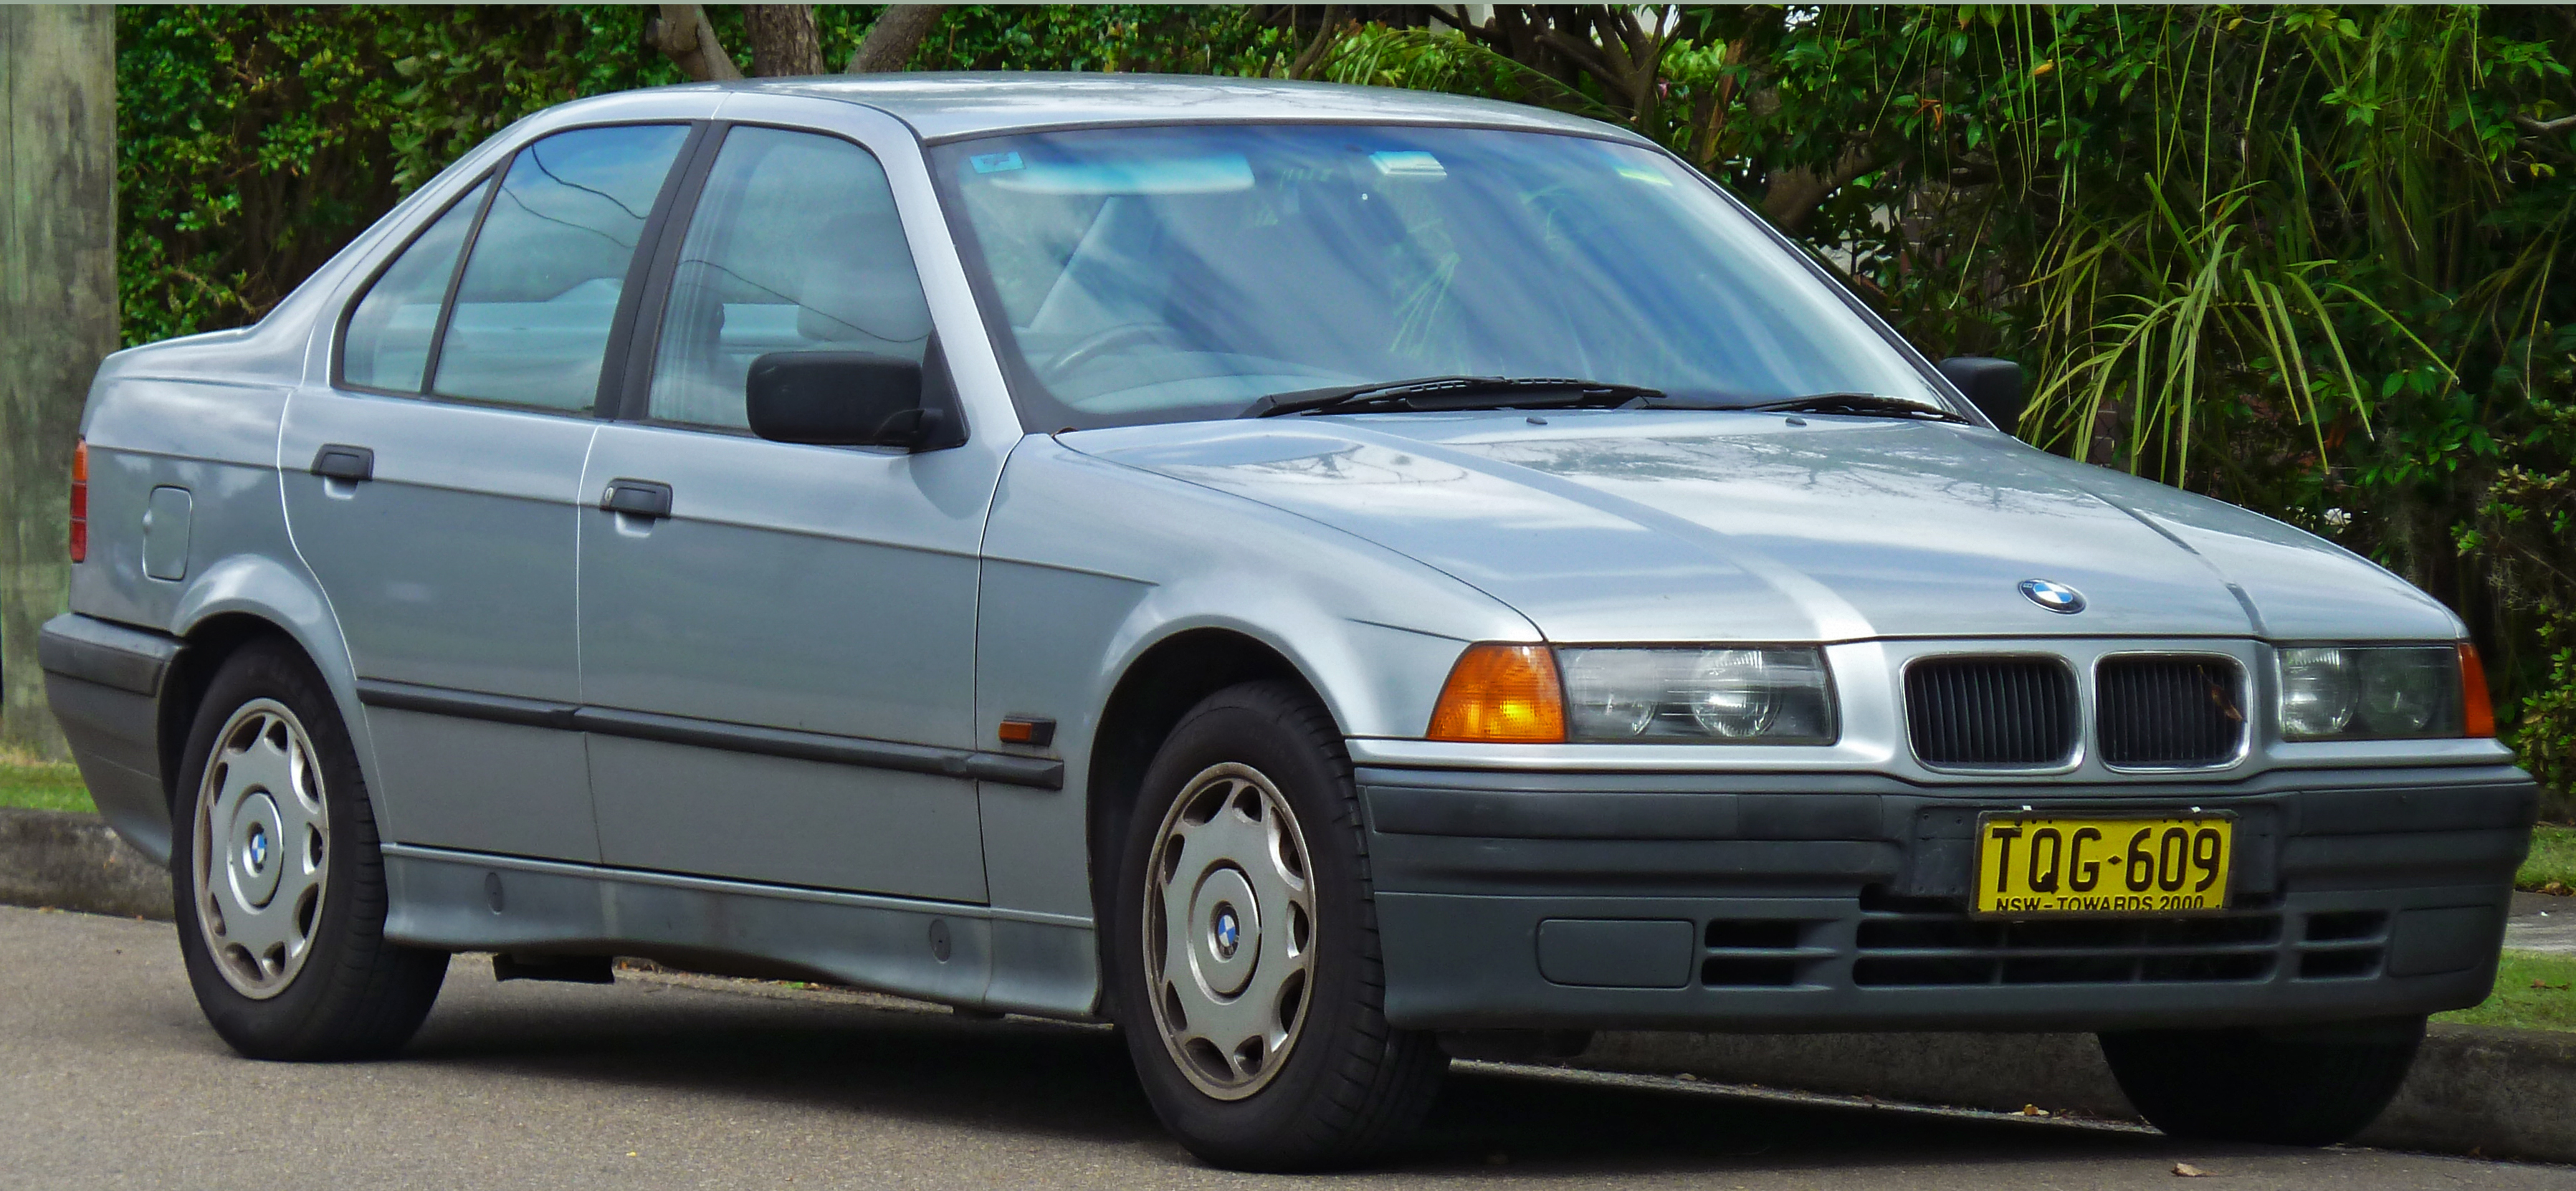
\includegraphics[width=1\textwidth]{img/e36.jpg} 
    
    \vspace{1em} % Adds spacing between image and quote
    
\caption[BMW Serie 3 E36]{Imágen de un vehículo BMW Serie 3 de la generación E36. Fuente: https://en.wikipedia.org/wiki/BMW\_3\_Series\_(E36).}
\label{fig:e36}
\end{figure}
    
\end{itemize}

Esta correspondencia (un mismo escenario de conducción aplicado a tres vehículos de masa, batalla y arquitectura de suspensión marcadamente distintas) es una demostración directa de la capacidad de reutilización que habilita el diseño modular de la biblioteca: simular un monoplaza de tracción trasera, a un hatchback de tracción delantera, o un sedan con puntal McPherson y eje multibrazo requiere solamente reemplazar el modelo del vehículo instanciado, sin alterar el entorno ni la estructura de la simulación.\\

El cuarto ejemplo, \verb|CarExampleUDP| está orientado a demostrar la visualización en tiempo real, utilizando un motor externo. Reutiliza el mismo \verb|Car| que \verb|CarExample|, pero añade cinco transmisores \verb|FrameToUDPOrientation|, uno para el chasis y uno por cada rueda, que emiten la pose completa (posición y orientación) a puertos UDP consecutivos del 12345 al 12349, de modo que un cliente en Unity (o cualquier otro visualizador) pueda renderizar elementos gráficos utilizando esta información en tiempo real. La señal de dirección es sinusoidal, para que el barrido de las ruedas pueda verificarse visualmente en el entorno gráfico. Debido a que los transmisores son sensores puros (no imponen fuerza y/o torque sobre los frames que leen), no alteran la dinámica del vehículo, y como los marcos de las ruedas se ubican sobre la salida de la junta de rotación, la orientación transmitida captura tanto el ángulo de dirección como el giro propio de cada rueda.\\


\subsection{CarExport}

El subpaquete \verb|Examples.CarExport| contiene los modelos de los tres vehículos listos para ser exportados y ejecutados desde un aplicación externa. Se diferencian de los otros ejemplos en el hecho de que no incorporan fuentes de señal, si no que exponen los comandos de entrada como inputs del modelo, para que un programa externo que gobierne la simulación los provea. Estos modelos son los que se exportan como FMU y los que usa la arquitectura de co-simulación descrita en la sección~\ref{sec:cosim}.\\

Los tres usan la clase parcial \verb|ExportInterface|, que declara la interfaz y no contiene ecuación alguna. Las entradas son los tres comandos normalizados del conductor y las salidas describen la pose de los cinco cuerpos que el visualizador necesita representar:

\begin{center}
\begin{tabular}{llcl}
\hline
\textbf{Conector} & \textbf{Tipo} & \textbf{Dim.} & \textbf{Contenido} \\
\hline
\verb|throttle| & \verb|RealInput| & 1 & acelerador, $[0,1]$ \\
\verb|steer|    & \verb|RealInput| & 1 & dirección, $[-1,1]$ \\
\verb|brake|    & \verb|RealInput| & 1 & freno, $[0,1]$ \\
\hline
\verb|r_chassis| & \verb|RealOutput| & 3 & posición del chasis \\
\verb|T_chassis| & \verb|RealOutput| & 9 & orientación del chasis \\
\verb|r_FL|, \verb|r_FR| & \verb|RealOutput| & 3 & posición de las ruedas delanteras \\
\verb|T_FL|, \verb|T_FR| & \verb|RealOutput| & 9 & orientación de las ruedas delanteras \\
\verb|r_RL|, \verb|r_RR| & \verb|RealOutput| & 3 & posición de las ruedas traseras \\
\verb|T_RL|, \verb|T_RR| & \verb|RealOutput| & 9 & orientación de las ruedas traseras \\
\hline
\end{tabular}
\end{center}

Cada vehículo exportado instancia el modelo del vehículo y el entorno \verb|Roads.Road|, conecta los cuatro marcos de rueda al contacto con el suelo, enlaza las tres entradas con las del vehículo y copia la pose de cada cuerpo a las salidas.

% Cada vehículo exportado instancia el modelo del automóvil y el entorno \verb|Roads.Road|, conecta los cuatro marcos de rueda al contacto con el suelo, enlaza las tres entradas con las del vehículo y, finalmente, copia la pose de cada cuerpo a las salidas. La matriz de rotación se aplana a un vector de nueve elementos, fila por fila, porque la interfaz de un FMU admite señales escalares y vectoriales pero no matrices. Reconstruirla del otro lado es reagrupar esos nueve valores, y el receptor puede además derivar de ellos un cuaternión si le resulta más cómodo para interpolar.\\

Exponer la orientación completa es lo que permite que el visualizador represente el guiñado, balanceo y cabeceo de la carrocería, además del giro propio de cada rueda.\\



\subsection{Resolución numérica del modelo}

Una vez traducido y compilado, el conjunto de componentes del sistema de simulación se convierte en eun sistema de ecuaciones algebráico-diferenciales (DAE). Además de las ecuaciones diferenciales que describen la dinámica de los cuerpos rígidos, el modelo contiene ecuaciones puramente algebráicas provenientes de las restricciones cinemáticas de los bucles cerrados de suspensión, resultantes de los ensamblajes \verb|JointRRR| y de las ecuaciones de acoplamiento entre conectores. La forma general de este sistema es implícita:
\begin{equation}
    F(t,\, y,\, \dot{y}) = 0
\end{equation}

donde $y$ es el vector de estados y $\dot{y}$ su derivada temporal. La integración de este sistema en el tiempo no puede realizarse de forma analítica, por lo que se recurre a métodos de integración numérica (\textit{solvers}). En el marco de OpenModelica se evaluaron dos solvers de referencia para la ejecución de la simulación: DASSL y CVODE. Ambos comparten la característica de ser especialmente adecuados para sistemas \textit{rígidos} (\textit{stiff}), condición que presenta el modelo del vehículo debido a la coexistencia de dinámicas de muy distinta escala temporal: las variaciones lentas del movimiento del chasis frente a las rápidas de la rigidez de contacto con el suelo y la regularización del frenado.

\subsubsection*{DASSL}

DASSL (\textit{Differential/Algebraic System Solver}) es el solver por defecto de OpenModelica, desarrollado por Petzold en Sandia National Laboratories \cite{petzold1982}. La principal ventaja es que opera directamente sobre la forma implícita  $F(t, y, \dot{y}) = 0$, más general que la forma explícita estándar $\dot{y} = f(t, y)$, lo que lo hace más apto ante sistema DAE como los que surgen del análisis dinámico de sistemas mecánicos multicuerpo. En particular, DASSL es aplicable incluso  cuando la matriz jacobiana $\partial F / \partial \dot{y}$ es singular, situación habitual en presencia de restricciones algebraicas.


El algoritmo se basa en la idea de Gear de reemplazar la derivada $\dot{y}$ en la ecuación implícita por una aproximación en diferencias, y resolver la ecuación no lineal resultante en el instante actual $t_n$ mediante el método de Newton. Para ello, emplea la fórmula de diferenciación regresiva (\textit{Backward Differentiation Formula}, BDF) de orden $k$, con $k$ variable entre $1$ y $5$. En su forma más simple, de primer orden, la aproximación es:

\begin{equation}
    F\!\left(t_n,\, y_n,\, \frac{y_n - y_{n-1}}{\Delta t_n}\right) = 0
\end{equation}

En cada paso, DASSL selecciona automáticamente tanto el orden $k$ como el tamaño de paso $\Delta t_n$ en función del comportamiento de la solución y de una estimación del error local de truncamiento, empleando además una formulación BDF de coeficiente líder fijo (\textit{fixed-leading-coefficient}) que mejora la estabilidad numérica. La ecuación no lineal se resuelve con una variante del método de Newton cuya matriz de iteración,

\begin{equation}
    G = \frac{\partial F}{\partial \dot{y}} + \alpha\, \frac{\partial F}{\partial y}
\end{equation}

donde $\alpha$ es un escalar que depende del paso y el orden. se factoriza y se reutiliza durante tantos pasos como sea posible para reducir el coste computacional. Su robustez frente a la forma DAE completa lo convierte en la opción de referencia para la validación del modelo.

\subsubsection*{CVODE}

CVODE (\textit{C-language Variable-coefficient ODE solver}) fue desarrollado por Cohen y Hindmarsh en Lawrence Livermore National Laboratory como una reescritura en C de los paquetes VODE y VODPK, y forma parte de la suite SUNDIALS \cite{cohen1995}. A diferencia de DASSL, CVODE resuelve el problema de valor incial de forma explícita $\dot{y} = f(t, y)$, por lo tanto, para su uso, el compilador de OpenModelica debe reducir previamente el sistema DAE a una forma de estado equivalente (índice 1 o forma ODE), operación que se apoya en la reducción de índice que aportan los ensamblajes analíticos de las suspensiones.

CVODE resuelve tanto sistemas rígidos como no rígidos mediante dos familias de métodos lineales multipaso de coeficiente, orden y paso variable: las fórmulas de Adams-Moulton (para problemas no rígidos, con orden entre $1$ y $12$) y las fórmulas BDF (para problemas rígidos, con orden entre $1$ y $5$). Ambas familias se expresan en la forma general:

\begin{equation}
    \sum_{i=0}^{K_1} \alpha_{n,i}\, y_{n-i} + h_n \sum_{i=0}^{K_2} \beta_{n,i}\, \dot{y}_{n-i} = 0
\end{equation}

donde para el caso BDF se tiene $K_1 = q$ y $K_2 = 0$, siendo $q$ el orden. En cada paso debe resolverse un sistema no lineal, que CVODE aborda mediante iteración funcional (para el caso no rígido, sin resolución de sistemas lineales) o mediante iteración de Newton (para el caso rígido). En este último caso, la iteración de Newton requiere resolver sistemas lineales con la matriz:

\begin{equation}
    M \approx I - \gamma\, J, \qquad J = \frac{\partial f}{\partial y}, \qquad \gamma = h_n\, \beta_{n,0}
\end{equation}

Para el tratamiento del jacobiano $J$ en el caso rígido, CVODE ofrece varias opciones: tratamiento denso, en banda, diagonal aproximado, o un método iterativo de Krylov (GMRES precondicionado), lo que le confiere gran flexibilidad y eficiencia. Su arquitectura modular, en la que el integrador principal es independiente del solver lineal empleado, junto con su condición de código moderno y activamente mantenido, lo convierten en una alternativa atractiva a DASSL para la búsqueda de un rendimiento adecuado en la ejecución en tiempo real.\\

\section{Interfaz para el hardware}

Para cerrar el bucle de simulación \textit{Man-in-the-Loop} es necesario capturar las acciones físicas del conductor sobre los dispositivos de entrada y traducirlas a input de control del modelo Modelica en tiempo real. Con este objetivo, se desarrolló una aplicación independiente en C++, cuya función es leer los periféricos de conducción, normalizar sus señales a un rango determinado (y estandarizado por el modelo de Modelica) y transmitirlas por red al motor de simulación. \\

La elección de utilizar una aplicación externa dedicada, en lugar de leer los inputs de los periféricos directamente desde Modelica responde a una separación de responsabilidades: el acceso al hardware de entrada es una tarea dependiente del sistema operativo y del driver/interfaz de cada dispositivo, independiente al dominio del modelado físico. Al desacoplar la adquisición de la simulación mediante un protocolo de red estándar, el modelo de Modelica permanece agnóstico con respecto del hardware utilizado y puede recibir entradas indistintamente de un periférico real, de una grabación reproducida o de un generador de señales sintético, además, permite la expansión y/o modificación del sistema de entrada, con la posibilidad de, por ejemplo, agregar la posibilidad de replicar el feedback enviado por Modelica hacia el hardware si se quisiese. El programa se organiza en una arquitectura por capas: \verb|core|, \verb|input|, \verb|model|, \verb|io|, \verb|ui| y \verb|app|, que aísla la adquisición de bajo nivel, la lógica de calibración, la comunicación de red y la interfaz de usuario en módulos independientes.


\subsection{Adquisición mediante DirectInput}

En esta aplicación, la captura de señales de los periféricos se realiza mediante la API \textit{DirectInput8}, desarrollada por Windows \cite{di}. Aunque se trata de una interfaz heredada dentro del ecosistema de Microsoft, sigue siendo el estándar para los volantes y pedaleras de simulación de conducción de gama comercial y permite ser utilizada en Linux mediante capas de compatibilidad como Wine o Proton, por lo que garantiza la compatibilidad con la mayor parte del hardware disponible en el mercado \cite{di,sdl}. DirectInput también establece una interfaz para interactuar con los servo-motores normalmente utilizados como dispositivos de entrada para los volantes de gama comercial, permitiendo así implementar un sistema para dar feedback proveniente del modelo si se quiere.\\


La lectura de cada dispositivo se realiza mediante \textit{polling}: en cada ciclo se invoca \verb|Poll|, seguido de \verb|GetDeviceState|, con la capacidad de reintentar la readquisición (\verb|Acquire|) del dispositivo ante alguna perdida inesperada (\verb|DIERR_INPUTLOST|), lo que provee robustez frente a desconexiones transitorias.

\begin{figure}[htbp]
    \centering
    % Replace 'example-image' with your file name
    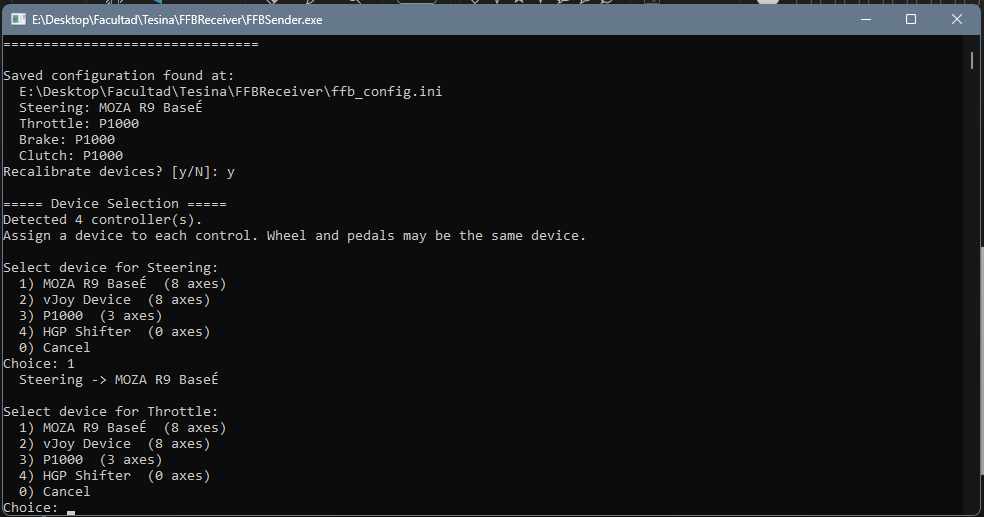
\includegraphics[width=1\textwidth]{img/device_selection.png} 
    
    \vspace{1em} % Adds spacing between image and quote
    
\caption[Selección de dispositivo]{Captura de la interfaz del sistema de envío de datos a la hora de mostrar y seleccionar el hardware para cada eje de input.}
\label{fig:device_selection}
\end{figure}


\subsection{Calibración y normalización de ejes}

Cada uno de los cuatro canales lógicos: dirección (\textit{steering}), acelerador (\textit{throttle}), freno (\textit{brake}) y embrague (\textit{clutch}), se asocia a un dispositivo y a un eje físico mediante un procedimiento de calibración interactivo de tres pasos:


\begin{enumerate}
    \item \textbf{Detección automática del eje.} Se solicita al usuario que accione el control a lo largo de todo su recorrido mientras el programa monitoriza el rango de los ocho ejes simultáneamente. El eje cuyo recorrido acumulado domina claramente sobre el resto se identifica como el eje asociado al canal. Este criterio de auto-escalado es robusto frente a diferencias de rango entre dispositivos y ante el ruido de los ejes en reposo.
    \item \textbf{Captura del rango.} Se registra el valor mínimo y máximo ($r_\text{min}$, $r_\text{max}$) alcanzado durante un barrido completo del control (de tope a tope en el volante, o de reposo a fondo en los pedales).
    \item \textbf{Confirmación de inversión.} Con una previsualización en vivo del valor normalizado, el usuario puede invertir el sentido del eje para que la convención de signo sea la correcta.
\end{enumerate}

La transformación de la lectura cruda $r$ a la señal de control normalizada aplica una función con recorte y, según el canal, una reescala bipolar o unipolar. Se define primero la fracción de recorrido:

\begin{equation}
    t = \operatorname{clamp}\!\left(\frac{r - r_\text{min}}{r_\text{max} - r_\text{min}},\; 0,\; 1\right)
\end{equation}

donde $\operatorname{clamp}(x, 0, 1)$ satura el valor al intervalo $[0, 1]$, evitando que lecturas fuera del rango calibrado produzcan salidas no deseadas. Tras aplicar opcionalmente la inversión, $t' = 1 - t$ si el eje está invertido, la salida final depende del modo del canal:

\begin{equation}
    y =
    \begin{cases}
        2\,t' - 1 & \text{modo bipolar (dirección),}\; y \in [-1, 1] \\[4pt]
        t'        & \text{modo unipolar (pedales),}\; y \in [0, 1]
    \end{cases}
\end{equation}

El modo bipolar mapea el volante de forma que su posición central corresponde a $y = 0$ y los topes a $-1$ hacia la izquierda, y $1$ hacia la derecha, el modo unipolar mapea cada pedal de forma de que la posición de reposo corresponde a $y=0$ y el fondo a $y=1$.  La configuración completa se persiste en un archivo \verb|ffb_config.ini|, de modo que la calibración solo debe realizarse una vez por configuración de hardware.\\
\newpage

\begin{figure}[htbp]
    \centering
    % Replace 'example-image' with your file name
    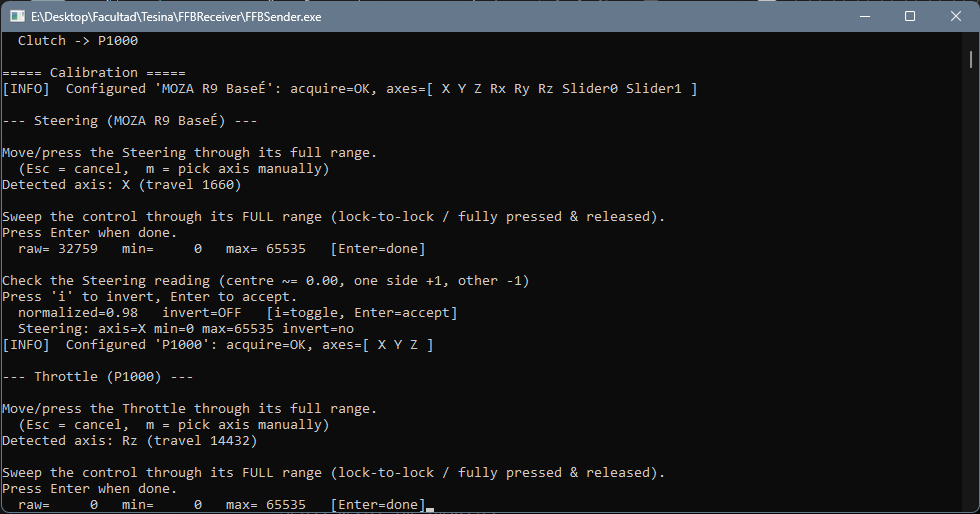
\includegraphics[width=1\textwidth]{img/calibration.png} 
    
    \vspace{1em} % Adds spacing between image and quote
    
\caption[Calibración de dispositivo]{Captura de la interfaz del sistema de envío de datos, mostrando el sistema de calibración del dispositivo.}
\label{fig:calibration}
\end{figure}


\subsection{Muestreo y transmisión en tiempo real}

El flujo de datos se obtiene ejecutando un hilo de trabajo dedicado que realiza un muestreo en intervalos determinados dependiendo de la frecuencia configurada, $\Delta t = 1000 / f_s$ ms, con un valor por defecto de $f_s = 100$ Hz que coincide con la frecuencia de sincronización en tiempo real del modelo Modelica. En cada ciclo, cada dispositivo de hardware se sondea exactamente una vez y su estado se comparte entre todos los canales (correspondientes a diferentes ejes) asociados a él. De este modo, los canales que provienen de un mismo periférico (por ejemplo, varios pedales de una misma pedalera) se muestrean de forma coherente en un único instante, sin desfase.\\

Los cuatro valores normalizados se transmiten mediante el protocolo UDP, en el caso de la computadora utilizada para las pruebas, que contiene Windows debido a la compatibilidad con los periféricos, se utiliza la biblioteca \textit{Winsock2}. Cada datagrama contiene exactamente $16$ bytes, correspondientes a cuatro números de punto flotante de $32$ bits (IEEE 754) en orden little-endian, concatenados sin cabecera:

\begin{center}
\begin{tabular}{cccc}
\hline
\textbf{Offset (bytes)} & \textbf{Longitud} & \textbf{Canal} & \textbf{Rango} \\
\hline
0  & 4 & \textit{steering} & $-1 \ldots 1$ \\
4  & 4 & \textit{throttle} & $0 \ldots 1$ \\
8  & 4 & \textit{brake}    & $0 \ldots 1$ \\
12 & 4 & \textit{clutch}   & $0 \ldots 1$ \\
\hline
\end{tabular}
\end{center}

La elección del protocolo UDP frente a TCP responde a los requisitos de una aplicación de control en tiempo real. TCP garantiza la entrega ordenada y sin pérdidas mediante confirmaciones y retransmisiones, pero a costa de una latencia variable e impredecible, un paquete perdido bloquea la entregas de los siguientes hasta su retransmisión. En un flujo de telemetría que corresponde a los inputs de un vehículo, un datagrama perdido pierde su significacncia una vez transcurrido su instante de muestreo, ya que el siguiente paquete lo reemplaza con información más reciente. UDP, al no tener confirmaciones de control ni de flujo, ofrece latencia mínima y determinista que exige la naturaleza de tener una simulación donde se tiene que poder reaccionar rápido a diferentes situaciones y que tiene que devolver feedback al conductor siendo la pérdida ocasional de un paquete un compromiso plenamente aceptable en este contexto, además de el hecho de que estos sistemas normalmente van a ejecutarse, o bien, en un mismo ordenador, o en una red local de alta velocidad, por lo que la perdida de paquetes sería mínima. \\


En el lado del receptor, el modelo Modelica lee el datagrama de $16$ bytes, desempaqueta los cuatro números de punto flotante en el mismo orden y los inyecta como las entradas \verb|steerInput|, \verb|speedInput| y \verb|brakeInput| del modelo del vehículo, cerrando así el lazo entre la acción física del conductor y la respuesta dinámica del vehículo simulado. Este canal de entrada opera de forma complementaria y en sentido inverso al flujo de salida descrito en la sección de interfaces (\verb|FrameToUDP|), que transmite la posición del vehículo hacia el visualizador.\\


Este programa fue creado como un ejemplo de una posible interfaz de entrada, como fue mencionado anteriormente, este programa puede ser reemplazado por otro, que funcione en diferentes sistemas operativos de forma nativa, o incluso en máquinas diferentes, siempre y cuando se respete el protocolo utilizado para transmitir información entre las partes del sistema.

\begin{figure}[htbp]
    \centering
    % Replace 'example-image' with your file name
    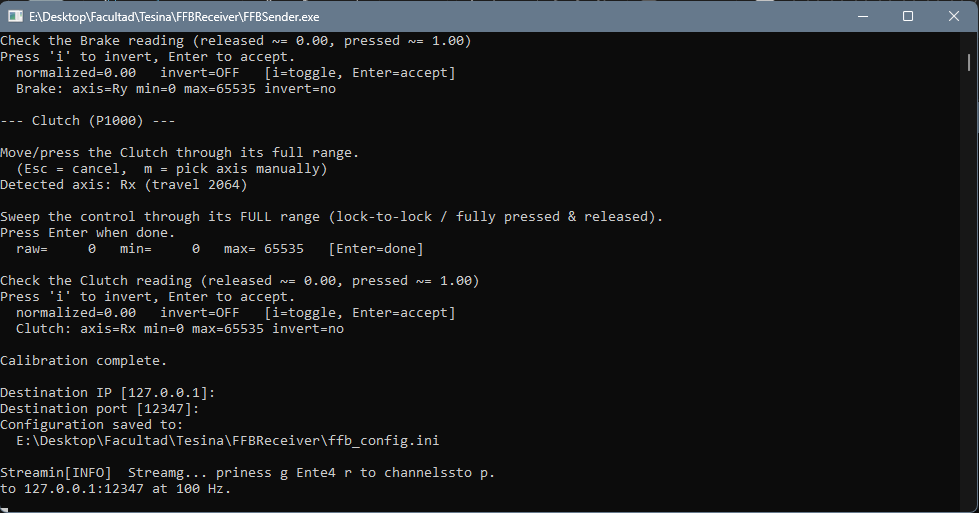
\includegraphics[width=1\textwidth]{img/running_data.png} 
    
    \vspace{1em} % Adds spacing between image and quote
    
\caption[Envío de información]{Captura de pantalla del estado del sistema de envío de datos cuando se termina la calibración de dispositivos y se comienza el envío de datos obtenidos del hardware.}
\label{fig:running_data}
\end{figure}

\section{Visualizador gráfico}
\subsection{El motor gráfico Unity}

Unity es un motor gráfco de desarrollo multiplataforma para aplicaciones interactivas en tiempo real, es ampliamente utilizado en la industria del videojuego.  Su arquitectura se organiza en torno a algunos conceptos fundamentales, definidos en su documentación oficial \cite{unity_docs}, que resultan necesarios para comprender la interfaz desarrollada:

\begin{itemize}
    \item \textbf{Escena y \textit{GameObjects}.} Una escena contiene un conjunto de objetos (\textit{GameObjects}), que son los contenedores básicos de todo elemento del mundo virtual, en este caso se utilizan para el chasis y las cuatro ruedas del auto.

    \item \textbf{Componente \textit{Transform}.} Cada \textit{GameObject} posee un componente \verb|Transform| que almacena la posición, rotación, escala y estado de jerarquía del objeto. Al modificar este componente, el objeto puede reposicionarse y reorientarse en la escena.
    
    \item \textbf{\textit{MonoBehaviour} y \textit{scripts}.} El comportamiento programable de un objeto se agrega mediante \textit{scripts} escritos en C\# que derivan de la clase base \verb|MonoBehaviour|. Esta clase expone una serie de funciones de ciclo de vida que el motor invoca automáticamente, como \verb|Start| (inicialización) y \verb|FixedUpdate| (actualización por intervalo).
    
    
    \item \textbf{Bucle de física \textit{FixedUpdate}.} A diferencia de \verb|Update|, que se ejecuta una vez por fotograma renderizado y por lo tanto su frecuencia varía dependiendo del rendimiento del computador, \verb|FixedUpdate| se invoca a intervalos fijos como parte del bucle de física del motor \cite{unity_docs} (por defecto cada 0{,}02 s, es decir, a 50 Hz), lo que garantiza un ritmo de actualización determinista, independiente de la tasa de refresco gráfico.

    
    \item \textbf{Sistema de coordenadas.} Unity emplea un sistema de coordenadas levógiro (sentido anti-horario) con el eje $Y$ apuntando hacia arriba, y representa las rotaciones internamente como cuaterniones. Esta convención difiere de la de Modelica, que es dextrógira (sentido horario) y también con $Y$ vertical, discrepancia que la interfaz debe resolver explícitamente.
\end{itemize}

\subsection{Interfaz de recepción de datos}

La interfaz que conecta Modelica con Unity se implementó como un \textit{script} de tipo \verb|MonoBehaviour| que recibe el flujo de pose emitido por el modelo de Modelica (ya sea por \verb|FrameToUDPOrientation| o por el orquestador del FMU) y lo aplica al \verb|Transform| del objeto correspondiente, modificando así su posición y orientación.  Se adjunta una instancia del \textit{script} a cada \textit{GameObject} para el chasis y cada una de las cuatro ruedas, configurando en cada una el puerto de escucha (\verb|listenPort|) para que coincida con el \verb|port_send| del transmisor Modelica asociado (12345 para el chasis y del 12346 al 12349 para las ruedas). De este modo, cada cuerpo rígido de la simulación se corresponde con un objeto de la escena y un flujo UDP dedicado.


\subsubsection*{Recepción concurrente}

La lectura de la red se ejecuta en un hilo de trabajo en segundo plano, independiente del hilo principal dedicado al renderizado del entorno. En su método \verb|Start|,  el \textit{script} abre un socket \verb|UdpClient| sobre el puerto configurado y lanza el hilo, que permanece bloqueado en la llamada de recepción a la espera de datagramas con información de posición. Esta separación es indispensable: si la recepción se realizara en el hilo principal, la llamada bloqueante detendría el renderizado hasta la llegada de cada paquete. La pose recibida se almacena en variables compartidas protegidas por un \textit{lock}, que garantiza el acceso seguro entre el hilo de red y el hilo de simulación.

\subsubsection*{Interpretación del datagrama}

Cada datagrama recibido se interpreta según el formato descrito en la sección de interfaces:  los primeros 12 bytes contienen la posición (tres flotantes de 32 bits) y, cuando el paquete alcanza los 28 bytes, los 16 bytes siguientes contienen el cuaternión de orientación (cuatro flotantes). El \textit{script} contempla ambos casos, aplicando únicamente la posición si el paquete es corto, lo que le permite operar indistintamente con los transmisores \verb|FrameToUDP| y \verb|FrameToUDPOrientation|.

\subsubsection*{Conversión de sistemas de coordenadas}

El núcleo de la interfaz es la conversión entre el sistema con sentido horario de Modelica y el de sentido anti-horario de Unity. Para la posición, la transformación consiste en negar la componente $Z$, conservando $X$ e $Y$:

\begin{equation}
    (x, y, z)_\text{Unity} = (x, y, -z)_\text{Modelica}
\end{equation}

Para la orientación, la misma inversión de eje ($S = \operatorname{diag}(1, 1, -1)$) se aplica a la rotación mediante la transformación de similitud $A_\text{Unity} = S\,A_\text{Modelica}\,S$, que sobre el cuaternión $(q_x, q_y, q_z, q_w)$, donde la parte escalar es $q_w$, equivale a negar las dos primeras componentes de la parte vectorial:

\begin{equation}
    (q_x, q_y, q_z, q_w)_\text{Modelica} \;\longrightarrow\; (-q_x, -q_y, q_z, q_w)_\text{Unity}
\end{equation}

Esta expresión fue una fuente de error durante el desarrollo: negar en su lugar la componente $q_z$ produce la rotación inversa, lo que se manifiesta visualmente como una precesión cónica del eje de giro de las ruedas en lugar de una rotación limpia.

\subsubsection*{Aplicación de la ubicación}

Finalmente, en el método \verb|FixedUpdate|, sincronizado con el bucle de física del motor, se lee la última ubicación recibida y se escribe sobre el \verb|Transform| del objeto: la posición de forma directa y la rotación componiéndola con un desfase de malla configurable (\verb|meshRotationOffset|). Este desfase corrige la discrepancia entre el eje geométrico de la malla y el eje físico del cuerpo, por ejemplo, para alinear el eje de un cilindro empleado como neumático (cuyo eje geométrico es su $Y$ local) con el eje de giro real de la rueda (su $Z$ local). El resultado es una representación tridimensional del vehículo que reproduce fielmente, y en tiempo real, la posición y la actitud calculadas por el modelo físico, incluyendo el ángulo de dirección y el giro propio de cada rueda.

\begin{figure}[htbp]
    \centering
    % Replace 'example-image' with your file name
    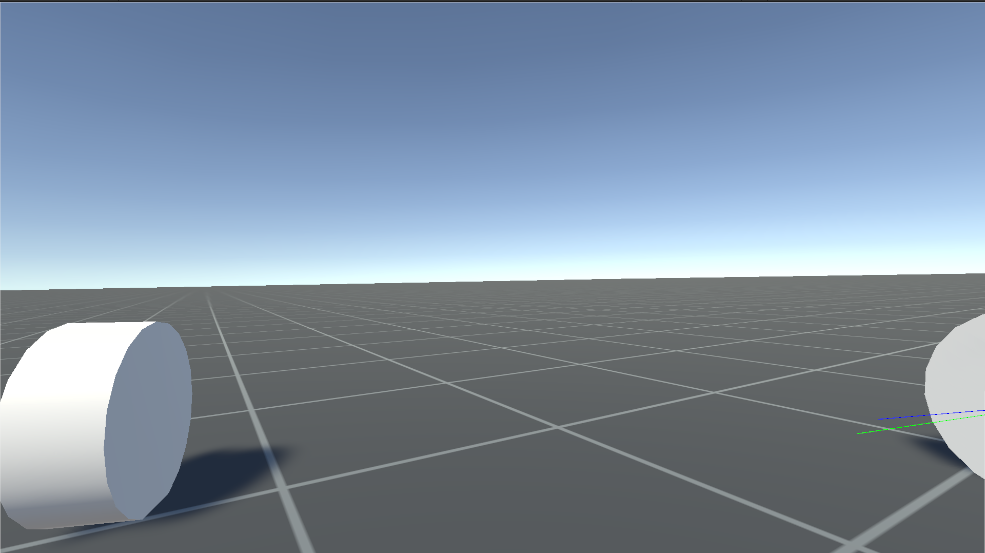
\includegraphics[width=1\textwidth]{img/unity.png} 
    
    \vspace{1em} % Adds spacing between image and quote
    
\caption[Entorno de Unity]{Captura de pantalla de la interfaz sencilla de Unity sincronizada con la información obtenida del modelo de Modelica. Se puede observar un entorno plano, con la cámara aproximadamente en la posición del conductor, y las dos ruedas delanteras moviéndose acorde a la dinámica del vehículo.}
\label{fig:running_data}
\end{figure}
\newpage


\section{Arquitectura de co-simulación}
\label{sec:cosim}

Las tres componentes explicadas hasta ahora deben ejecutarse simuláneamente e intercambiar información al ritmo configurado para el lazo/simulación. La forma aparentemente más directa, y que se tomó como primer acercamiento, fue usar las herramientas presentadas para que envíen y reciban paquetes UDP mediante los bloques del paquete \verb|Interfaces|. Esta sección explica por qué esa vía resultó inviable con el compilador empleado y describe la arquitectura que finalmente se adoptó.

\subsection{Por qué el modelo no puede cerrar el lazo por sí mismo}

Un lazo cerrado que incluye interacción humana necesita muestrear su entrada, el comando del conductor llega en instantes discretos y debe mantenerse constante entre ellos. En Modelica, esto se representa con una cláusula \verb|when sample(...)|, presente tanto en \verb|UDPReceive| como en \verb|UDPSend| y en \verb|RealtimeSynchronize|.

El hallazgo que determinó el cambio en la arquitectura original fue que la simple presencia de un reloj periódico de muestreo en el modelo impide a CVODE integrar más allá de un lapso de tiempo determinado, en este caso fueron diecinueve segundos. Cabe remarcar que algunos cambios en la interfaz de entrada/salida hacían que ese valor cambie, pero con un mismo modelo, este siempre abortaba al mismo instante de tiempo. Esto no se debe a un problema del modelo del vehículo ni del volumen de datos, este mismo error se puede replicar colocando tres bloques \verb|Sampler| transmitiendo valores constantes, sin conexión alguna con el resto del sistema.  El Apéndice~\ref{sec:appendix} documenta el caso mínimo de reproducción.

 % El Apéndice~\ref{sec:appendix} documenta el caso mínimo de reproducción junto con los otros dos defectos del compilador que se encontraron en el curso de este trabajo.

Dado que muestrear dentro del modelo es la causa del problema, la solución consistió en moverlo fuera del sistema de ecuaciones.


% \subsection{Un paso intermedio: comunicación sin Modelica\_DeviceDrivers}

% Antes de llegar a esa conclusión se implementaron versiones de los bloques de comunicación que reemplazan la cadena de \textit{Modelica\_DeviceDrivers} por una única función externa en C. El modelo \verb|UDPInputDirect| sustituye la secuencia \verb|UDPReceive| seguida de cuatro \verb|GetFloat| por una función \verb|udpRead4| que abre un \textit{socket} no bloqueante, lo drena y devuelve el último datagrama disponible; \verb|FrameToUDPDirect| hace lo propio en el sentido de la transmisión con una función \verb|udpSend7|. Ambas conservan el formato de los paquetes, de modo que los programas del otro extremo no requieren modificación alguna.

% Estas versiones eliminan una falla distinta y anterior —una detención a los $2{,}6$ s con los bloques originales— y reducen el sistema en unas $620$ ecuaciones, pero no resuelven la limitación de fondo: siguen necesitando un reloj de muestreo. Se conservan en la biblioteca porque suprimen la dependencia de una biblioteca externa en el camino crítico y porque documentan el defecto en ambos sentidos de la comunicación.

\subsection{El modelo como FMU de intercambio de modelos}

La solución implementada consiste en exportar el modelo del vehículo como una \textit{Functional Mock-up Unit} (FMU) siguiendo el estándar FMI~2.0, y trasladar el muestreo, la integración y la sincronización a una aplicación externa. El modelo se convierte en una biblioteca que contiene una función de avance explícita, es decir, nada sucede en él hasta que el programa que lo instancia se lo pida.

Se emplea la variante de intercambio de modelos (\textit{Model Exchange}) y no la de co-simulación. Un FMU de co-simulación incluye a su propio integrador, lo que resulta más cómodo, pero los generados por  OpenModelica~1.25.5 terminan abruptamente durante el avance de la integración. Por lo que para agilizar el desarrollo, se utilizó este tipo de FMU que no contiene integrador, si no que expone las derivadas del estado y es la aplicación externa la que integra, lo que permite utilizar una implementación independiente que no presenta problemas.

El modelo exportado (\verb|Examples.CarExport|) es un wrapper del vehículo y del entorno en el que se encuentra, y expone hacia afuera tres entradas \verb|steer|, \verb|throttle| y \verb|brake|, además de que por cada uno de los cinco cuerpos (cuatro ruedas y el chasis) expone su posición en el sistema de referencia global, con su orientación. Esto resulta en un modelo que expone lo mismo que se recibía/enviaba por UDP pero sin contener bloques de comunicación, ni de muestreo y con la animación deshabilitada para obtener un mejor desempeño.

La orientación se exporta como una matriz de rotación de nueve componentes y no como cuaternión. El motivo es por una falla del compilador: la conversión \verb|Frames.to_Q| hace fallar al generador de código FMI con un error de dimensiones incompatibles aunque el mismo modelo compila y simula sin dificultad como ejecutable autónomo. La conversión a cuaternión para compatibilizarlo con el visualizador se hace en la aplicación de control, copiando la implementación de \verb|Quaternions.from_T| para que el paquete transmitido resulte idéntico al que emitía el modelo original.


% La exportación se automatiza con un guion que fija la configuración necesaria:

% \begin{verbatim}
% buildModelFMU(DDynamics.Examples.CarExport.CarExport,
%               version = "2.0", fmuType = "me",
%               fileNamePrefix = "CarExport", platforms = {"static"});
% \end{verbatim}

% Conviene señalar dos detalles que no son evidentes. La instrucción es \verb|buildModelFMU| y no \verb|translateModelFMU|: esta última solo traduce el modelo, informa éxito y no genera archivo alguno. Y la opción \verb|platforms| con el valor \verb|static| enlaza el binario de forma estática, de modo que el FMU no dependa de que las bibliotecas dinámicas de OpenModelica estén disponibles al momento de ejecutarlo.

\subsection{La aplicación de control}

La aplicación de control (o \textit{master}) es el programa que se encarga de controlar el lazo. Se ubica entre la interfaz de hardware y el visualizador, comunicándose con ambos por UDP, según muestra la Figura~\ref{fig:cosim}.

\begin{figure}[H]
\centering
\begin{tikzpicture}[font=\small,
    box/.style={draw, rounded corners=2pt, minimum height=1.2cm,
                align=center, inner sep=6pt},
    ar/.style={-{Latex[length=2mm]}, thick}]

  \node[box, fill=black!5]  (ffb) at (0,0)   {\texttt{FFBSender}\\{\footnotesize volante y pedales}};
  \node[box, fill=black!12, line width=1pt] (mas) at (6,0) {aplicación de control\\{\footnotesize FMU + integrador}};
  \node[box, fill=black!5]  (uni) at (12,0)  {Unity\\{\footnotesize visualizador}};

  \draw[ar] (ffb) -- node[above, font=\scriptsize, align=center]
      {UDP 12344\\$4\times$float32} (mas);
  \draw[ar] (mas) -- node[above, font=\scriptsize, align=center]
      {UDP 12345--12349\\$7\times$float32} (uni);
\end{tikzpicture}
\caption[Arquitectura de co-simulación]{Arquitectura del lazo cerrado. El muestreo, la integración y la sincronización con el reloj de pared ocurren en la aplicación de control, fuera del sistema de ecuaciones del modelo. Los formatos de los paquetes son los que ya emitía y esperaba cada extremo, de forma que ni la interfaz de hardware ni el visualizador requirieron modificación.}
\label{fig:cosim}
\end{figure}

Su bucle principal, con un paso de comunicación configurable de $10$ ms por defecto, realiza en cada iteración cuatro operaciones: escribe en el FMU el último comando recibido, avanza la integración en un paso, lee las poses de los cinco cuerpos, las encola para su transmisión y espera hasta el instante que indique su frecuencia. 

 % El comando se mantiene constante durante todo el paso, lo que constituye el mismo retenedor de orden cero que antes rompía a CVODE, con la diferencia esencial de que ahora ocurre entre llamadas al integrador y no como un evento temporal dentro de las ecuaciones.

La aplicación se estructura en tres hilos: uno para recibir los comandos del conductor, otro para ejecutar la integración y el último que se encarga de transmitir las poses. La principal ventaja de esto es que una lectura bloqueante de red no detiene la ejecución del integrador.



% Dos decisiones de diseño merecen mención. El hilo de recepción conserva únicamente el datagrama más reciente y descarta los anteriores: en un lazo en tiempo real un comando viejo no tiene valor alguno. Y un vigilante anula los comandos si no llega ningún datagrama durante medio segundo, de modo que la caída del programa de adquisición no deje aplicado indefinidamente el último valor de acelerador.


\subsection{Bibliotecas empleadas en la aplicación de control}

La aplicación de control se implementó en Python. La estructura de comunicación y concurrencia se resuelve utilizando la biblioteca estándar del lenguaje, sin incluir dependencias externas. La única dependencia de tercero es la que permite el acceso al modelo.

\subsubsection{FMPy}

FMPy es una implementación del estándar FMI en Python \cite{fmpy} y es la que permite cargar el FMU e interactuar con él. Se emplean dos componentes: el primero es la interfaz de bajo nivel \verb|FMU2Model|, que expone directamente las funciones de la norma (fijar entradas, leer y escribir el vector de estados, obtener las derivadas y los indicadores de evento, gestionar el modo de eventos). Se recurre a esta interfaz y no a la de simulación por lotes porque el lazo cerrado requiere inyectar comandos entre pasos sucesivos, algo que una llamada por lotes no permite.

El segundo componente utilizado es \verb|CVodeSolver|, un enlace a la biblioteca SUNDIALS \cite{hindmarsh2005} que provee el integrador CVODE \cite{cohen1995}. Este es el mismo algoritmo empleado en OpenModelica, pero con una implementación y entorno diferente, lo que nos permite evitar ciertos problemas que presentaba el entorno de OpenModelica, que resultaron claves para la ejecución de algunos experimentos.

 % es precisamente esa independencia la que permite eludir los defectos del entorno de OpenModelica documentados en el Apéndice~\ref{sec:appendix}.


% \subsubsection{El estándar FMI}

% El formato de intercambio está definido por la especificación 

% \paragraph{El estándar FMI.} El formato de intercambio está definido por la especificación FMI~2.0 \cite{blochwitz2012}, que fija tanto la estructura del archivo —el descriptor \verb|modelDescription.xml| y los binarios compilados— como la interfaz en C que el FMU expone. Que ambos extremos se atengan a un estándar es lo que hace posible combinar un modelo generado por OpenModelica con un integrador provisto por otra herramienta.

\subsubsection{Sobre la elección del lenguaje}
Utilizar el lenguaje Python para controlar el lazo en tiempo real merece justificación. Las únicas operaciones que la aplicación ejecuta en Python puro son la lectura de las poses, su conversión a cuaternión y una llamada a un callback de la librería SUNDIALS, que consumen entre el $5$ y el $7\%$ del tiempo de cada iteración. El resto del costo corresponde a la integración, que ocurre dentro del código compilado en C de SUNDIALS. La elección del lenguaje entonces no penaliza demasiado el desempeño y además simplifica la instrumentación y los experimentos. Cabe además aclarar, que si se requiere obtener más desempeño en el sistema, esta aplicación puede ser reemplazada por otra compilada en algún otro lenguaje, siempre y cuando respete los estándares de comunicación entre las partes y el protocolo FMI~2.0 \cite{blochwitz2012}.

% Emplear un lenguaje interpretado para gobernar un lazo en tiempo real merece justificación, y la medición la aporta. Las únicas operaciones que la aplicación ejecuta en Python puro son la lectura de las poses, su conversión a cuaternión y una llamada a un callback de la librería SUNDIALS, que consumen entre el $5$ y el $7\,\%$ del tiempo de cada iteración. La totalidad del costo restante corresponde a la integración, que ocurre dentro del código compilado en C FMU. La elección del lenguaje no penaliza, por lo tanto, el desempeño del lazo, y a cambio simplifica notablemente la instrumentación y los experimentos.


\subsection{Consecuencias de la arquitectura}

El resultado es un sistema en el que el modelo deja de incluir bloques de comunicación y sincronización y en el que las tres partes del sistema se comunican exclusivamente mediante UDP con formatos fijos. Se mantiene la libertad de poder modificar cualquiera de ellas sin tocar al resto: el programa de adquisición podría reemplazarse por otro periférico o por una entrada sintética, y el visualizador por un motor gráfico distinto, siempre que respeten los formatos de la Figura~\ref{fig:cosim}. 

Realizar este cambio, sumado a pasar la responsabilidad de la sincronización con el tiempo real a la aplicación de control, simplifica la arquitectura del modelo en Modelica, dejando solamente que este se encargue de cumplir su función principal: modelar un sistema físico, y dejando las funcionalidades de red a otros programas que estén más adaptados a cumplir esas responsabilidades.

% La sincronización con el tiempo real pasa a ser una espera en el bucle de la aplicación de control, por lo que el bloque \verb|RealtimeSynchronize| pasa a ser innecesario, lo que elimina el pro

% El acompasamiento con el tiempo real pasa a ser una espera en el bucle de la aplicación de control, lo que además vuelve innecesario el bloque \verb|RealtimeSynchronize| y elimina el problema de tener cinco instancias del mismo compitiendo por acompasar una única simulación. La contrapartida es que la responsabilidad de la integración —la elección del integrador, su tolerancia y el tamaño del paso de comunicación— se traslada del compilador a la aplicación, y con ella la necesidad de caracterizar su desempeño, que es el objeto del Capítulo~\ref{sec:experiments}.


\chapter{Experimentos}
\label{sec:experiments}
\section{Simulación de Lazo Abierto}
\section{Costo computacional de la simulación}

El objetivo de esta tesina es desarrollar un simulador capaz de ejecutarse en tiempo real, con el feedback del conductor dentro del lazo. Esta condición implica que el tiempo de cómputo necesario para avanzar la simulación un intervalo $\Delta t$ debe ser menor que $\Delta t$ medido en el reloj real. Esta sección apunta a medir en qué grado los modelos desarrollados cumplen con dicho requisito, y compara los integradores numéricos seleccionados en OpenModelica para este tipo de sistema. Primero se va a evaluar el sistema de lazo abierto, y luego se va a realizar una medición más específica con el entorno completo.


\subsection{Protocolo de medición}

Para obtener las mediciones se ejecutó cada uno de los tres modelos desarrollados (\verb|CivicEKCar|, \verb|E36Car| y \verb|Car|, este último referido como FF1600 por el monoplaza en el que se basa) realizando los mismos inputs, que generan una maniobra idéntica y deliberadamente exigente computacionalmente:

\begin{itemize}
    \item Horizonte de simulación de $10$ s.
    \item Comando de dirección al tope derecho ($\text{steer} = 1$) durante toda la maniobra.
    \item Acelerador al máximo ($\text{throttle} = 1$) desde el instante inicial.
    \item Aplicación del freno al máximo ($\text{brake} = 1$) a partir de $t = 5$ s.
\end{itemize}

La maniobra combina saturación simultánea de demanda longitudinal y lateral ya que el vehículo acelera en un giro de radio mínimo (en teoría) hasta la mitad del intervalo y frena en esa misma condición durante el resto. Es un caso desfavorable de forma intencional, ya que lleva al neumático al límite del círculo de fricción, donde la saturación de la fuerza de contacto introduce la no linealidad más severa del modelo.

Cada modelo se evaluó sobre dos geometrías de terreno, una superficie plana y otra que generaba una superficie sinusoidal, con los dos integradores mencionados anteriormente (DASSL y CVODE), con el agregado de \verb|gbode| en algunos casos, con el objetivo de comparar contra otra familia de solver. Se registran dos magnitudes: el tiempo \textit{total}, que incluye la inicialización del sistema y la escritura de resultados, y el tiempo de \textit{simulación}, correspondiente al tiempo de avance de la integración.  Las mediciones se realizaron sobre el ejecutable ya compilado, de modo que el tiempo de traducción y compilación del modelo queda excluido, ya que no son relevantes a la ejecución en tiempo real.

\subsection*{Resultados}

La tabla~\ref{tab:tiempos} grafica las mediciones. El símbolo $\dagger$ marca las ejecuciones que abortaron antes de alcanzar los $10$ s de simulación establecidos, en esos casos el valor registrado corresponde al tiempo total de ejecución de la simulación hasta la falla y por lo tanto no es una medida de tiempo comparable con las ejecuciones que completaron correctamente.


\begin{table}[H]
\centering
\begin{tabular}{llcccccc}
\hline
 & & \multicolumn{3}{c}{Tiempo total (s)} & \multicolumn{3}{c}{Tiempo de simulación (s)} \\
Terreno & Solver & Civic & E36 & FF1600 & Civic & E36 & FF1600 \\
\hline
\multirow{2}{*}{Plano}
 & DASSL & 1{,}468 & 1{,}658 & 0{,}396$^\dagger$ & 1{,}152 & 1{,}339 & 0{,}329$^\dagger$ \\
 & CVODE & 0{,}793 & 0{,}654 & 0{,}780 & 0{,}756 & 0{,}619 & 0{,}741 \\
\hline
\multirow{2}{*}{Sinusoidal}
 & DASSL & 0{,}323$^\dagger$ & 0{,}502$^\dagger$ & 2{,}353$^\dagger$ & 0{,}238$^\dagger$ & 0{,}411$^\dagger$ & 1{,}984$^\dagger$ \\
 & CVODE & 4{,}184 & 1{,}867 & 1{,}486 & 4{,}095 & 1{,}805 & 1{,}435 \\
\hline
\end{tabular}

\caption[Tiempos de ejecución de los modelos de vehículo]{Tiempos de ejecución para una maniobra de $10$ s con dirección al tope, acelerador máximo y frenada máxima a partir de $t = 5$ s, con tolerancia relativa $10^{-6}$. $^\dagger$ La ejecución abortó antes de completar la simulación, el valor indica el tiempo hasta la falla y no es comparable con el de una corrida completa.}
\label{tab:tiempos}
\end{table}

La figura~\ref{fig:tiempos} representa gráficamente los tiempos de simulación de la tabla. Se omiten las barras de las ejecuciones que no completaron correctamente.

\begin{figure}[H]
\centering
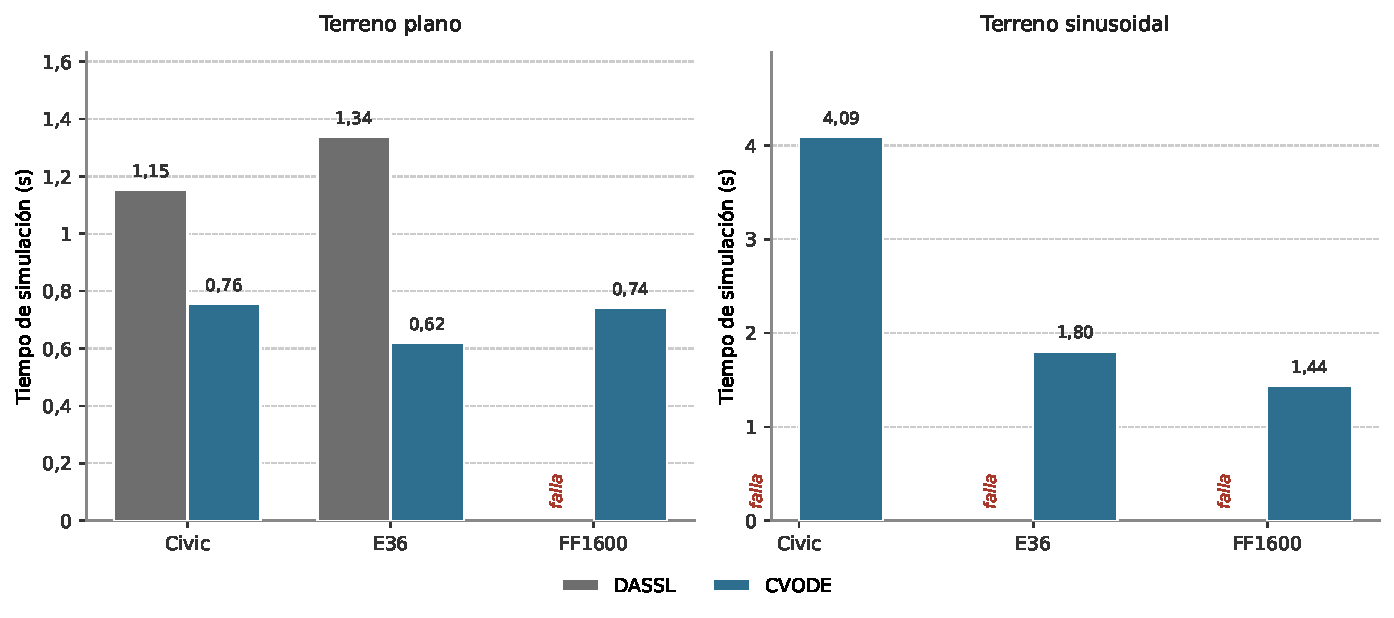
\includegraphics[width=\textwidth]{img/tiempos_simulacion.pdf}


\caption[Tiempo de simulación por vehículo, solver y terreno]{Tiempo de simulación para la maniobra de $10$ s. Las entradas marcadas como \textit{falla} corresponden a ejecuciones que abortaron antes de completar la simulación y por lo tanto no se grafican: DASSL falla con el modelo FF1600 sobre terreno plano y con los tres vehículos sobre terreno sinusoidal. CVODE completa las seis configuraciones.}
\label{fig:tiempos}
\end{figure}

El resultado más interesante para la tesina no es el tiempo absoluto, si no, como se compara este con el tiempo total de la simulación, ya que una relación menor a 1x limita la capacidad de ejecutar un entorno en tiempo real. La Figura~\ref{fig:tiemporeal} expresa las mediciones de CVODE (ya que fue el único integrador en completar todas las configuraciones) como factor un coeficiente entre el tiempo total de la simulación y el tiempo que tardó en ejecutarse. La línea discontinua en $1\times$ marca la frontera del tiempo real: por encima de ella la simulación avanza más rápido que el reloj y, por lo tanto, admite operación con el conductor dentro del lazo.


\begin{figure}[H]
\centering
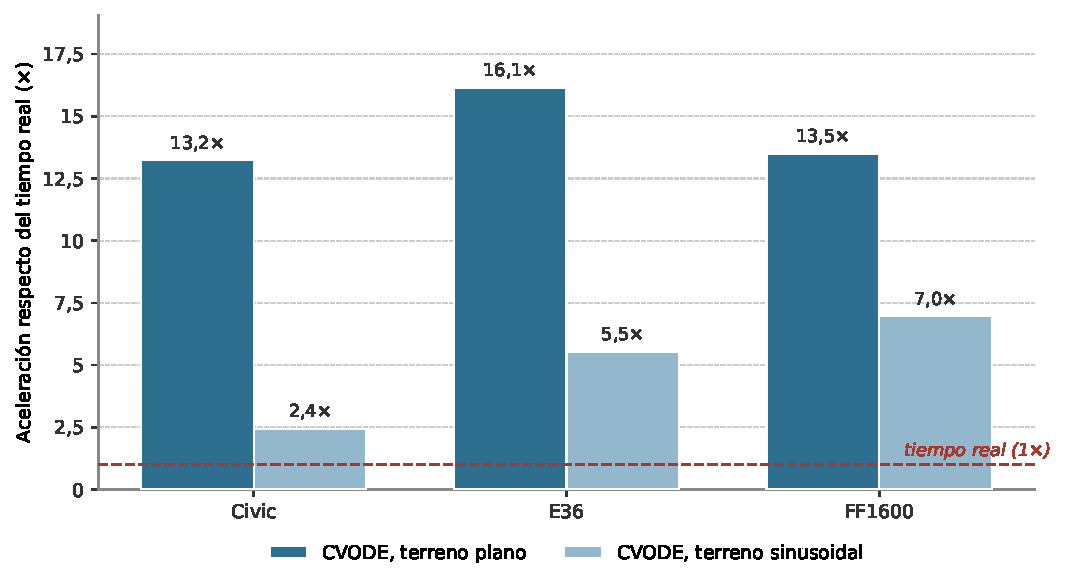
\includegraphics[width=0.86\textwidth]{img/tiempo_real.pdf}
\caption[Aceleración respecto del tiempo real]{Factor de aceleración respecto del tiempo real de los tres modelos de vehículo con CVODE, definido como el cociente entre el horizonte simulado ($10$ s) y el tiempo de cómputo. La línea discontinua marca el umbral de tiempo real: todos los casos se sitúan por encima, con márgenes entre $2{,}4\times$ y $16{,}1\times$.}
\label{fig:tiemporeal}
\end{figure}

\subsection{Complejidad de los modelos}

Para interpretar mejor los tiempos, conviene tener una medida del tamaño de cada modelo. La tabla~\ref{tab:complejidad} muestra el número de ecuaciones del sistema plano (obtenido usando la instrucción \verb|checkModel| de OpenModelica) junto con el número de estados continuos e indicadores de evento (leídos de la descripción \verb|modelDescription.xml| del FMU exportado).

\begin{table}[H]
\centering
\begin{tabular}{lrrrr}
\hline
Modelo & Ecuaciones & Triviales & Estados & Ind. de evento \\
\hline
\verb|Car| (FF1600) & 12\,269 & 8\,585 & 30 & 8 \\
\verb|CivicEKCar|   & 12\,269 & 8\,584 & 30 & 8 \\
\verb|E36Car|       &  9\,897 & 6\,746 & 30 & 8 \\
\hline
\end{tabular}

\caption[Complejidad de los modelos de vehículo]{Tamaño de cada modelo de vehículo. Las ecuaciones triviales son las que el compilador resuelve por sustitución directa y no llegan al sistema que resuelve el integrador. Los estados continuos y los indicadores de evento se obtuvieron de la descripción del FMU exportado de cada modelo.}
\label{tab:complejidad}
\end{table}

El dato más relevante de la tabla es que los tres vehículo tienen exactamente el mismo número de estados continuos, a pesar de que utilizan topologías distintas. Esto es debido al uso del componente  \verb|JointRRR| señalada en la Sección~\ref{sec:method}: al resolver analíticamente el bucle cinemático, no introduce restricciones ni variables de estado adicionales. Los treinta estados corresponden a los seis grados de libertad del chasis, los cuatro recorridos de suspensión y los cuatro giros de rueda, con sus respectivas derivadas, independientemente de que la suspensión sea de doble triángulo, McPherson o multibrazo. A notar también de que tanto el FF1600 como el CivicEKCar contienen la misma cantidad de ecuaciones, a pesar de ser vehículos completamente distintos en papel, sin embargo, su topología de suspensión es la misma (doble triángulo en las cuatro esquinas). 


\subsection{Sensibilidad a la tolerancia}

La tolerancia relativa del integrador es el parámetro que controla el compromiso entre exactitud y costo computacional. Para tener una mejor idea sobre que valor utilizar, se repitió la maniobra sobre el terreno sinusoidal (ya que es el más exigente) con CVODE y tolerancias de $10^{-4}$, $10^{-6}$ y $10^{-8}$. Los resultados se presentan en la Tabla~\ref{tab:tolerancia} y la Figura~\ref{fig:tolerancia}.

\begin{table}[H]
\centering
\begin{tabular}{lcccccc}
\hline
 & \multicolumn{3}{c}{Tiempo total (s)} & \multicolumn{3}{c}{Tiempo de simulación (s)} \\
Tolerancia & Civic & E36 & FF1600 & Civic & E36 & FF1600 \\
\hline
$10^{-4}$ & 2{,}473 & 1{,}015 & 0{,}963 & 2{,}232 & 0{,}804 & 0{,}728 \\
$10^{-6}$ & 4{,}767 & 1{,}555 & 1{,}487 & 4{,}549 & 1{,}375 & 1{,}271 \\
$10^{-8}$ & 7{,}721 & 2{,}582 & 2{,}446 & 7{,}508 & 2{,}405 & 2{,}232 \\
\hline
\end{tabular}
\caption[Sensibilidad del costo a la tolerancia del integrador]{Tiempos con CVODE sobre terreno sinusoidal para tres tolerancias relativas.}
\label{tab:tolerancia}
\end{table}

\begin{figure}[H]
\centering
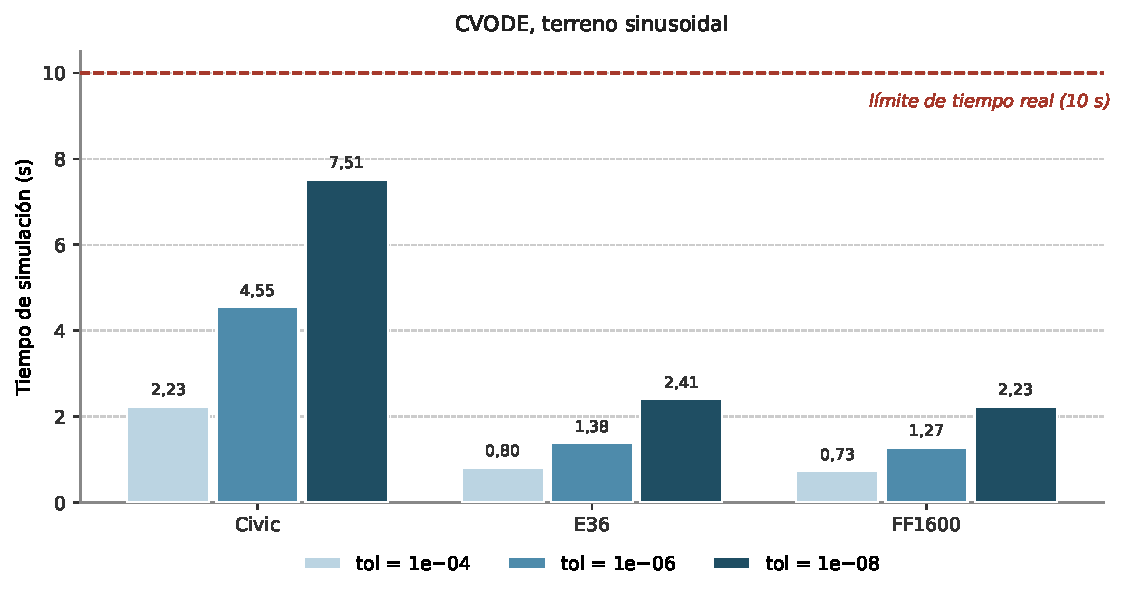
\includegraphics[width=0.86\textwidth]{img/tolerancia.pdf}
\caption[Costo en función de la tolerancia del integrador]{Tiempo de simulación con CVODE sobre terreno sinusoidal para tolerancias de $10^{-4}$, $10^{-6}$ y $10^{-8}$. La línea discontinua marca el límite de tiempo real: una barra que la supere indicaría que la simulación no puede sostener el ritmo del reloj. Ninguna configuración lo alcanza, ni siquiera con la tolerancia más estricta.}
\label{fig:tolerancia}
\end{figure}

El costo crece de forma regular: cada dos órdenes de magnitud de tolerancia adicional, se multiplica el tiempo de cómputo por un factor de entre $1{,}7$ y $2{,}0$.  \\

Comparando contra el tiempo real, incluso utilizando la tolerancia más estricta se preserva el margen: la relación contra el reloj con $10^{-8}$ es de $1{,}3\times$ para el Civic y $4{,}5\times$ para el FF1600, contra $12{,}4\times$ y $13{,}7\times$ respectivamente con $10^{-4}$. La elección de la tolerancia $10^{-6}$ para el resto de los experimentos se dio debido a que es un punto medio: conserva un buen margen contra el tiempo real, permitiendo más overhead para incluir carga adicional proveniente del resto del entorno, manteniendo un nivel de tolerancia aceptable. \\

% Vale la pena aclarar la falla del modelo E36 con $10^{-8}$, ya que es diferente a las fallas vistas anteriormente de DASSL. El error indica que el número de iteraciones del evento superó el límite establecido por default (veinte), lo que sugiere un encadenamiento de eventos que no llegan a converger (\textit{chattering}) y no una divergencia de la integración. Esto es debido a que al exigir mayor exactitud, el solver coloca los cruces por cero con más precisión, y detecta conmutaciones que con tolerancias mayores quedaban enmascaradas dentro del error admitido. Este límite es configurable mediante el indicador de tiempo de ejecución \verb|-mei=<valor>|, pero aumentar ese valor no resolvería la causa original, la mejor forma de solucionar esto es encontrar cuál es la conmutación responsable y suavizarla, del mismo modo que se hizo con la regulación a la resistencia a la rodadura, o con los frenos, descrito en la sección~\ref{sec:method}.


\subsection{Exactitud de la solución}

La sección anterior se dedicó a mostrar lo que cuesta aumentar la tolerancia, todavía queda por determinar cuanto se gana con ello. Para medirlo, se comparó con cada modelo, la trayectoria obtenida con diferentes tolerancias contra la tolerancia más escrita que se pudo correr en el modelo, para tomarla como referencia. 

El experimento se realizó de forma diferente al protocolo utilizado anteriormente, las principales diferencias fueron:

Las ejecuciones se realizaron sobre los FMU mediante la biblioteca \verb|fmpy| y no sobre el ejecutable de OpenModelica. La justificación es que el FMU admite tolerancias más estrictas. Utilizando esta metodología los tres vehículos pueden ejecutarse hasta  $10^{-10}$, valor que se toma como referencia. 

Los inputs de la simulación fueron reemplazados por una maniobra suave (dirección $0{,}2$ y acelerador $0{,}3$ constantes, sin frenada) en lugar de la maniobra extrema del benchmark de costo. Esto se realizó debido a que, utilizando los inputs anteriores, el neumático opera en el límite (y superando) de fricción, lugar donde las trayectorias vecinas divergen. Por lo tanto, utilizar la maniobra agresiva sirve para medir la divergencia del sistema, pero no es la mejor forma de medir la exactitud del integrador. Además, al ser una maniobra menos extrema, el tiempo de cómputo es menor, por lo que esta métrica no es directamente comparable con los de la tabla~\ref{tab:tolerancia}, que corresponden a otra maniobra y otro terreno.

Por último, todas las corridas se interpolan sobre una grilla temporal común. Fijar el intervalo de ejecución no es suficiente, porque \verb|fmpy| agrega una muestra por cada evento y el número de estos (y por lo tanto de entradas) varía según la tolerancia especificada. Los instantes de la grilla utilizada están presentes en los datos originales, de forma que la interpolación no introduce error de remuestreo.

Las medidas utilizadas para medir el error de la trayectoria son: el error de posición del chasis al final del intervalo de simulación $\lVert \mathbf{r}(T) - \mathbf{r}_\text{ref}(T) \rVert$, y el error cuadrático medio sobre toda la trayectoria normalizado por el desplazamiento total del vehículo (NRMSE), que hace comparables vehículos que recorrer distancias distintas. La Tabla~\ref{tab:exactitud} reúne los resultados y la Figura~\ref{fig:errorposicion} los representa.

\begin{table}[H]
\centering
\begin{tabular}{llccc}
\hline
Modelo & Tolerancia & Error final (m) & NRMSE (\%) & Razón de mejora \\
\hline
\multirow{3}{*}{FF1600}
 & $10^{-4}$ & $1{,}85\times10^{-2}$ & $1{,}8\times10^{-2}$ & --- \\
 & $10^{-6}$ & $4{,}68\times10^{-5}$ & $4{,}7\times10^{-5}$ & $395$ \\
 & $10^{-8}$ & $7{,}59\times10^{-7}$ & $<10^{-5}$ & $62$ \\
\hline
\multirow{3}{*}{E36}
 & $10^{-4}$ & $1{,}44\times10^{-2}$ & $9{,}4\times10^{-3}$ & --- \\
 & $10^{-6}$ & $2{,}30\times10^{-4}$ & $2{,}2\times10^{-4}$ & $63$ \\
 & $10^{-8}$ & $2{,}26\times10^{-6}$ & $<10^{-5}$ & $102$ \\
\hline
\multirow{3}{*}{Civic}
 & $10^{-4}$ & $2{,}25\times10^{-2}$ & $1{,}8\times10^{-2}$ & --- \\
 & $10^{-6}$ & $2{,}75\times10^{-4}$ & $1{,}7\times10^{-4}$ & $82$ \\
 & $10^{-8}$ & $1{,}12\times10^{-6}$ & $<10^{-5}$ & $245$ \\
\hline
\end{tabular}
\caption[Exactitud de la solución en función de la tolerancia]{Error respecto de la solución de referencia, calculada con tolerancia $10^{-10}$, para una maniobra suave de $10$ s. La razón de mejora es el cociente entre el error de la fila anterior y el de la fila actual. Los desplazamientos totales recorridos son de $42{,}9$ m (FF1600), $48{,}9$ m (E36) y $50{,}0$ m (Civic).}
\label{tab:exactitud}
\end{table}

\begin{figure}[H]
\centering
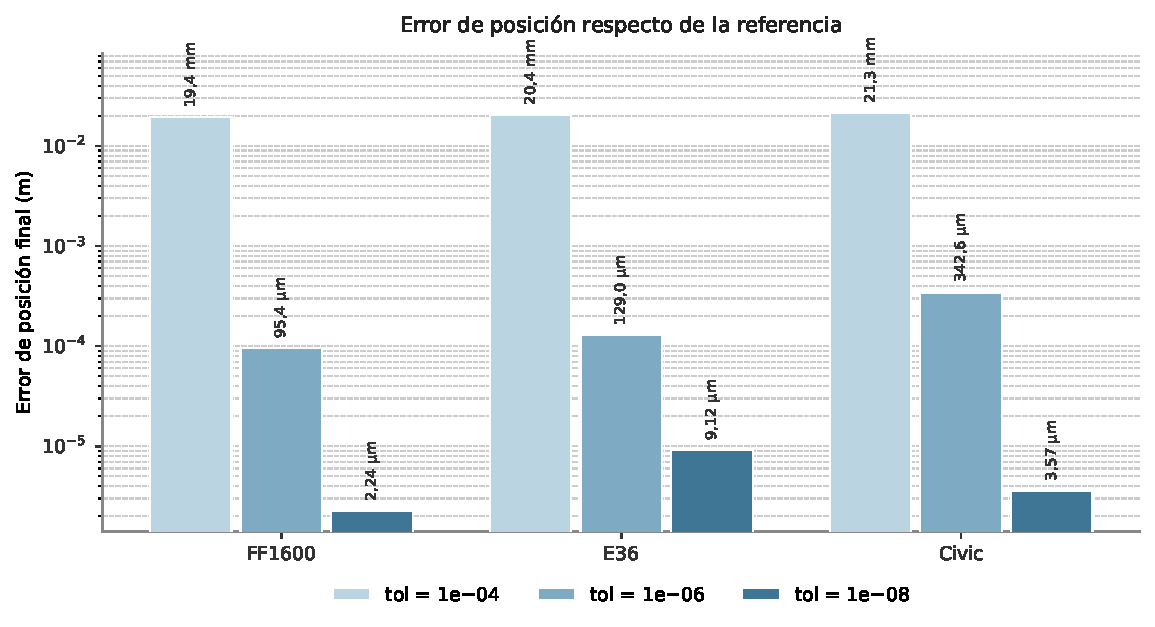
\includegraphics[width=0.86\textwidth]{img/error_posicion.pdf}
\caption[Error de posición en función de la tolerancia]{Error de posición del chasis al cabo de $10$ s respecto de la solución de referencia con tolerancia $10^{-10}$, en escala logarítmica. Sobre cada barra se indica el valor en unidades legibles.}
\label{fig:errorposicion}
\end{figure}

El comportamiento es el esperado, cada dos décadas de tolerancia el error se reduce aproximadamente dos órdenes de magnitud. Esta convergencia regular es evidencia de que la integración se comporta correctamente sobre este modelo.

En términos absolutos, las cifras son aceptables para el objetivo del simulador. Con la tolerancia $10^{-6}$ elegida, el error de posición al cabo de diez segundos de simulación es de $47$ a $275$ micrómetros sobre recorridos de unos cincuenta metros, equivalente un NRMSE inferior al $0{,}0002\text{\%}$. Incluso con la tolerancia más baja ensayada, $10^{-4}$, el apartamiento máximo es de $2{,}3$ cm, un valor que es imperceptible para un conductor e inferior a la incertidumbre de los propios parámetros del modelo (masas, rigideces y coeficientes de fricción) que se conocen con una precisión mucho menor. La tolerancia deja de ser el factor limitante de la fidelidad del simulador y en mi opinión pasaría a ser, por un lado, el conocimiento con mayor exactitud de las características del vehículo y por otro, una mayor fidelidad a la hora de plasmar ciertos aspectos de este, por ejemplo, eliminando la abstracción del chasis como un paralelepípedo e intercambiándola por algo más preciso.

Vale la pena mencionar que en casi todos los casos el error máximo sobre la trayectoria coincide con el error del final, lo que indica que este crece de forma monótona a lo largo de la maniobra, mostrando de que es un error acumulativo por truncamiento.



% Por último, una limitación del método: la referencia se obtiene con el mismo integrador que las soluciones evaluadas, de modo que lo que se mide es la \textit{convergencia} del esquema al refinar la tolerancia y no su exactitud frente a un método independiente. Un error sistemático común a todas las tolerancias no sería detectado por esta prueba. Una verificación cruzada exigiría contrastar contra DASSL sobre terreno plano, el único escenario en el que ese integrador resulta estable.

\subsection{Comparación de integradores}

Las mediciones de exactitud de la sección anterior compara CVODE contra sí mismo, por lo que mide la convergencia del sistema al modificar la tolerancia, pero no detectaría si hubiera un error común en el solver, independientemente de los parámetros. Esta sección agrega la verificación cruzada con otros solvers, comparando tres diferentes sobre el mismo modelo y maniobra.

Los integradores utilizados fueron: CVODE y DASSL, ambos de la familia de (BDF) y \verb|gbode|, de la familia de métodos Runge-Kutta de OpenModelica. Agregar el tercer método responde a una necesidad de agregar un solver que no comparta familia con los dos anteriores, para evitar ocultar errores posibles debido a la naturaleza de los sistemas, por lo que agregar un método de Runge-Kutta descarta esa posibilidad. 

Las ejecuciones se vuelven a correr como al principio de esta sección, utilizando el ejecutable de OpenModelica y no sobre el FMU. Esto es debido a dos razones, la primera es que \verb|fmpy| no ofrece ni DASSL ni \verb|gbode|, y la segunda es metodológica: comparar el CVODE de \verb|fmpy| contra el DASSL de OpenModelica agrega una segunda variable, el entorno de simulación, por lo que se decidió volver a realizar todo sobre un mismo entorno.


Se emplea la misma maniobra suave utilizada en la pureba de exactitud, por la misma razón que fue explicada en ese estudio. Las tolerancias son $10^{-4}$ y $10^{-6}$. Como OpenModelica escribe una grilla equidistante y el indicador \verb|-noEventEmit| suprime las muestras de evento, las mediciones caen exactamente sobre los mismos instantes, y por lo tanto no se requiere interpolación alguna. Cada configuración se repite tres veces para el tiempo de cómputo.


\begin{table}[H]
\centering
\begin{tabular}{llcc}
\hline
Modelo & Integrador & Tol. $10^{-4}$ & Tol. $10^{-6}$ \\
\hline
\multirow{3}{*}{FF1600}
 & CVODE & $0{,}49 \pm 0{,}02$ & $0{,}60 \pm 0{,}00$ \\
 & DASSL & falla$^{\S}$ & falla$^{\S}$ \\
 & gbode & $10{,}46 \pm 0{,}27$ & $12{,}97 \pm 0{,}34$ \\
\hline
\multirow{3}{*}{E36}
 & CVODE & $0{,}34 \pm 0{,}00$ & $0{,}38 \pm 0{,}00$ \\
 & DASSL & $0{,}38 \pm 0{,}00$ & $0{,}43 \pm 0{,}01$ \\
 & gbode & $4{,}98 \pm 0{,}14$ & $7{,}03 \pm 0{,}07$ \\
\hline
\multirow{3}{*}{Civic}
 & CVODE & $0{,}43 \pm 0{,}00$ & $0{,}53 \pm 0{,}00$ \\
 & DASSL & $0{,}48 \pm 0{,}01$ & $0{,}67 \pm 0{,}01$ \\
 & gbode & $1{,}30 \pm 0{,}01$ & $2{,}22 \pm 0{,}00$ \\
\hline
\end{tabular}
\caption[Tiempo de cómputo de los tres integradores]{Tiempo de cómputo en segundos (media $\pm$ desviación estándar de tres repeticiones) para la maniobra suave de $10$ s. $^{\S}$ Aborta a los $0{,}29$ s.}
\label{tab:solvers}
\end{table}

CVODE sigue siendo el solver más rápido en todas las configuraciones que completa:  DASSL cuesta entre $1{,}1$ y $1{,}3$ veces más, y \verb|gbode| entre $3$ y $22$ veces más. La diferencia era esperable en el caso de \verb|gbode|, cuyos métodos Runge-Kutta implícitos resuelven varios sistemas no lineales por paso.

Sigue habiendo una diferencia de robustez más marcada que de costo, pero concentrada en un único modelo, CVODE y \verb|gbode| completan todas las configuraciones, DASSL, sin embargo, falla en ambas pruebas del monoplaza.

% La brecha de robustez sigue siendo más marcada que la de costo, pero se concentra en un único modelo. CVODE y \verb|gbode| completan las seis configuraciones cada uno; DASSL falla en dos, ambas del monoplaza y con las dos tolerancias ensayadas. El aborto se produce a los $0{,}29$ s, durante el transitorio de asentamiento inicial y no en régimen establecido, lo que sugiere que la dificultad está en la fase en que la suspensión recorre su rango completo antes de estabilizarse. El diagnóstico es el mismo de siempre, \textit{«linear system solver failed»}, y no depende de la tolerancia, lo que descarta que se trate de un problema de control de error.

% Sin embargo, la diferencia más grande está en la robustez,  CVODE completa las seis configuraciones; \verb|gbode| falla en una; DASSL falla en dos, ambas del modelo E36 y con las dos tolerancias ensayadas. Es notable remarcar que DASSL aborta en el E36 incluso con la maniobra suave, cuando en el benchmark de costo solo fallaba sobre terreno sinusoidal, su fragilidad sobre este modelo no se limita a los regímenes de saturación.

La tabla~\ref{tab:acuerdo} y la figura~\ref{fig:acuerdo} presentan la diferencia entre pares de integradores con tolerancia $10^{-6}$, junto con el error propio de CVODE contra si mismo utilizando una tolerancia de $10^{-10}$, que sirve de comparación.

\begin{table}[H]
\centering
\begin{tabular}{lccc|c}
\hline
Modelo & CVODE--DASSL & CVODE--gbode & DASSL--gbode & Error propio de CVODE \\
\hline
FF1600 & ---       & $10{,}8$  & ---       & $46{,}8$  \\
E36    & $67{,}9$  & $87{,}6$  & $135{,}4$ & $229{,}6$ \\
Civic  & $95{,}2$  & $72{,}2$  & $164{,}3$ & $274{,}8$ \\
\hline
\end{tabular}
\caption[Diferencia entre integradores]{Diferencia de posición final entre pares de integradores, en micrómetros, con tolerancia $10^{-6}$. La última columna es el error de CVODE respecto de su propia referencia $10^{-10}$ (Tabla~\ref{tab:exactitud}). Los pares en que se usa DASSL no se informan para el monoplaza, porque ese integrador aborta sobre ese modelo.}
\label{tab:acuerdo}
\end{table}

\begin{figure}[H]
\centering
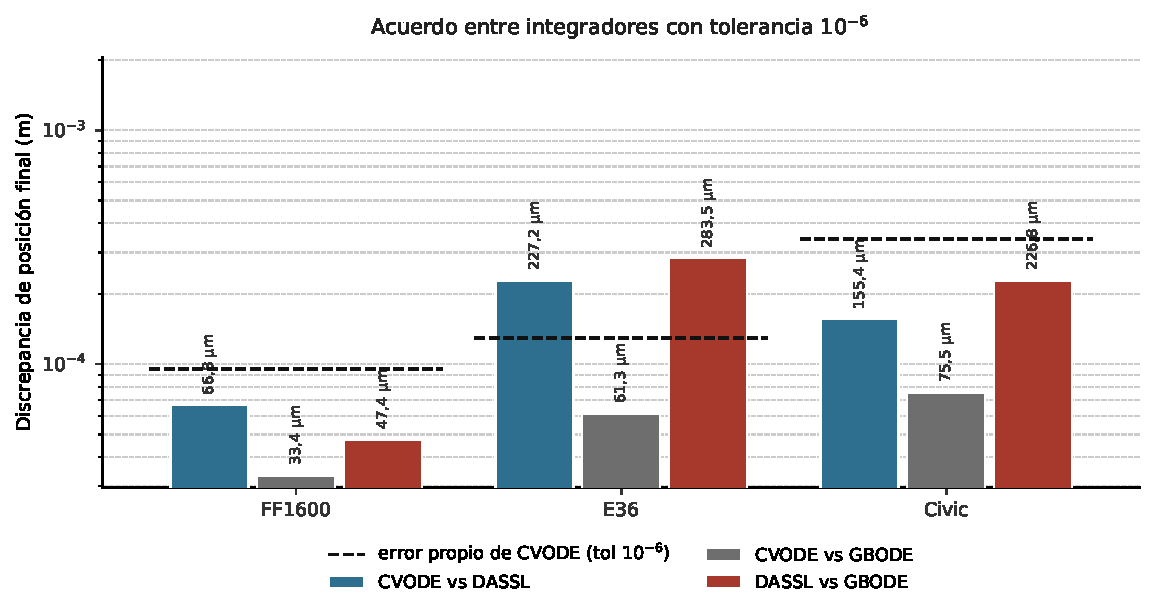
\includegraphics[width=0.86\textwidth]{img/solvers_acuerdo.pdf}
\caption[Acuerdo entre integradores]{Diferencia de posición final entre pares de integradores con tolerancia $10^{-6}$, en escala logarítmica. La línea discontinua marca, para cada vehículo, el error propio de CVODE a esa tolerancia: las diferencias del mismo orden indican acuerdo dentro de la exactitud alcanzable.}
\label{fig:acuerdo}
\end{figure}

El resultado es el buscado. Las diferencias entre pares de solver van de  $10{,}8$ a $164{,}3$ micrómetros, es decir, el mismo orden de magnitud que el error propio de CVODE frente a su referencia, de $46{,}8$ a $274{,}8$ micrómetros. Los tres métodos coinciden dentro de la exactitud que cada uno alcanza a esa tolerancia, no se detecta ningún sesgo generado por algún integrador en particular. Y dado que \verb|gbode| pertenece a otra familia de métodos, la coincidencia no puede explicarse por un problema compartido de la formulación BDF.

Con la tolerancia en $10^{-4}$ las diferencias crecen dos órdenes de magnitud, hasta $23{,}6$ mm, lo que también es consistente ya que el error propio de cada método es mayor de todas forams. El acuerdo entre integradores empeora en la misma proporción que la exactitud individual.

% La excepción vuelve a ser el modelo E36, que no admite verificación cruzada porque es el único que ningún otro integrador puede hacer que complete correctamente. El encadenamiento de eventos con tolerancias bajas refuerza de que puede ser un problema del modelo en sí y no del integrador. Queda pendiente identificar la conmutación responsable, probablemente en los topes de suspensión de la topología \verb|MultiLink|, queda como trabajo pendiente.


\subsection{Discusión}

\subsubsection{Robustez antes que velocidad}



% El hallazgo más significativo de este capítulo no es de rendimiento, si no de robustez. En el benchmark de costo DASSL aborta en cuatro de seis configuraciones, en la comparación de integradores falla en dos de seis y \verb|gbode| en una. CVODE, sin embargo, completa las doce configuraciones ejecutadas en ambos experimentos sin una sola falla.

Lo habitual al elegir un integrador es negociar entre velocidad y robustez. Sin embargo en este caso, CVODE es al mismo tiempo el más rápido (entre $1{,}1$ y $1{,}3$ veces más que DASSL, y entre $3$ y $22$ veces más que \verb|gbode|) y el único que no presenta fallas en las ejecuciones. Por lo tanto, la elección resulta sencilla y CVODE se adopta como integrador de referencia de la biblioteca.

\subsubsection{La tolerancia dejó de ser el factor limitante}

Los resultados de las pruebas de costo y exactitud proveen un resultado claro con respecto al ajuste de la tolerancia. Por el lado del costo, cada dos décadas de tolerancia agregada se duplica el tiempo de cómputo. Por el lado de la exactitud, estas mismas dos décadas reducen el error en dos órdenes de magnitud. El intercambio es favorable a ajustar la tolerancia y no existe razón de rendimiento para relajarla demasiado.
 
La medición mas relevante para observar es la magnitud absoluta del error. Con la tolerancia elegida de $10^{-6}$ la trayectoria se aparta de la referencia entre $47$ y $275$ micrómetros al cabo de diez segundos de simulación en el entorno ejecutado, e incluso con la tolerancia más permisiva, el error máximo es de $2{,}3$ cm. Ambas cifras son órdenes de magnitud menores que la incertidumbre con las que se conocen los parámetros físicos del modelo (masas, rigideces, coeficientes de fricción, geometría de la suspensión). El esfuerzo de mejora, rinde mucho más si es aplicado a la caracterización del vehículo antes que al control del error del integrador.

\subsubsection{Las conmutaciones son la dificultad numérica dominante}

Hay un patrón que se repite en todos los experimentos realizados: la dificultad numérica observada se atribuye a una no linealidad conmutativa y no al tamaño del sistema ni a la complejidad cinemática.

Se observó que la saturación del círculo de fricción degrada la convergencia de un factor $41$ a un factor $3{,}3$, haciendo que se invalide la maniobra agresiva para la prueba de exactitud.

La lección aprendida con estas pruebas es que rinde más invertir esfuerzo en suavizar de forma controlada las conmutaciones antes que ajustar los parámetros del integrador. Una discontinuidad que se encuentra en una condición de operación habitual puede costar más que el resto del modelo.



\subsubsection{Costo del terreno irregular}

Para CVODE, pasar de terreno plano al de la forma sinusoidal multiplica el tiempo de simulación por factores de entre $1{,}9$ (FF1600) y $5{,}4$ (Civic). Esto es consistente con lo esperado del modelo de contacto, sobre superficie plana la penetración del neumático se estabiliza en un valor casi constante, mientras que en el perfil sinusoidal oscila de forma continua, obligando al integrador a reducir el paso. Un detalle a tener en cuenta es que este terreno es una exageración de lo que se puede ver en la vida real, por lo que se debe tomar como un caso del peor escenario posible.

\subsubsection{Costo de inicialización}

La diferencia entre el tiempo total y el de simulación se puede usar para comparar el costo fijo de inicialización y escritura de resultados. Para CVODE se sitúa entre $0{,}034$ y $0{,}090$ s, mientras que para DASSL alcanza aproximadamente $0{,}32$ s. Este costo es irrelevante para estas pruebas ya que es una simulación por lotes, pero para el caso de tiempo real se puede ver como un retraso antes de comenzar la simulación interactiva, sin embargo, ambos son tiempos de espera asumibles.


\subsubsection{Complejidad del modelo y costo}

Contrastando los tiempos contra la tabla~\ref{tab:complejidad} se pueden observar dos efectos separados. El primero responde al tamaño del modelo: el E36 tiene $19{,}3\text{\%}$ menos de ecuaciones comparado a los otros vehículos (debido a su suspensión \verb|McPherson|, construida sobre una única articulación \verb|Prismatic| para simplificar) y es el más rápido de ejecutar sobre terreno plano.\\

El segundo efecto no se puede explicar de la misma forma. Los modelos \verb|Car| y \verb|CivicEKCar| tienen el mismo número de ecuaciones ($10\,981$), el mismo número de estados ($30$) y la misma topología de suspensión en las cuatro esquinas, pero sobre terreno sinusoidal el Civic tarda $2{,}85$ veces más que el FF1600. Dado que el tamaño del sistema es fijo, esa diferencia solo puede provenir del número de pasos que el integrador necesitar dar debido a la rigidez numérica que introducen los parámatros utilizados en el modelo. La masa suspendida, la rigidez del muelle y el amortiguamiento determinan la frecuencia del conjunto y en consecuencia el paso máximo admisible. El Civic, con $990$ kg de masa suspendida sobre muelles de $16$ y $14$ kN/m, presenta una dinámica vertical más exigente de seguir que el monoplaza de $400$ kg.\\

La conclusión es que el costo de estos modelos tiene dos componentes independientes: el tamaño del sistema en sí y la rigidez de la dinámica, y que reducir el primero no reduce necesariamente el segundo.


\subsubsection{Qué limita realmente al simulador}

Reuniendo todo lo anterior, la capacidad de cómputo no es la restricción principal que tiene este simulador. Con márgenes de entre $2{,}4\times$ y $16{,}1\times$ respecto del tiempo real sobre la maniobra más exigente y con un error de integración de centésimas de milímetro, ni la velocidad ni la exactitud del integrador son los factores que pueden acatar la calidad del resultado.

Las principal restricción que posee el modelo es su robustez, un modelo puede resultar numéricamente frágil con independencia del margen de cómputo disponible.

Este margen extra se puede invertir, en las pruebas de lazo cerrado, parte de este se va a ir a la ejecución tanto de las interfaces como de el entorno gráfico. Sin embargo, el margen es lo suficientemente grande como para agregar modelos de neumático o de suspensión más detallados, o la simulación simultánea de varios vehículos sin comprometer la operación interactiva.


% \subsection*{Limitaciones de la medición}

% Los tiempos del \textit{benchmark} de costo —Tablas~\ref{tab:tiempos} y \ref{tab:tolerancia}— corresponden a una única ejecución por configuración, sin repeticiones, por lo que no se dispone de una estimación de su dispersión. El estudio de exactitud sí repite cinco veces cada configuración, con desviaciones estándar de entre $0{,}01$ y $0{,}13$ s, lo que da una idea del orden de la variabilidad esperable también en aquellas mediciones. En una máquina de propósito general, con planificación de procesos y estados de caché variables, la variabilidad entre corridas idénticas puede ser significativa. Las conclusiones cualitativas —el orden de magnitud del margen respecto del tiempo real, y sobre todo el patrón de fallas de DASSL, que es determinista— son robustas frente a esa incertidumbre; las comparaciones finas entre vehículos, en cambio, deberían respaldarse con la media y la desviación estándar sobre un número suficiente de repeticiones.

% Debe señalarse además que un valor medio de tiempo por paso, aun holgadamente inferior al umbral de tiempo real, no garantiza por sí solo una experiencia interactiva satisfactoria: lo que percibe el conductor es el peor caso, no el promedio.


\section{Simulación a lazo cerrado}

Todas las mediciones anteriores son simulaciones por lotes, el modelo se ejecuta con una maniobra predefinida y se observan los resultados luego de que esta termina. En esta sección se va a medir el sistema completo en funcionamiento, con el volante y pedales físicos generando comandos al vehículo y el visualizador de Unity recibiendo las poses. Esta medición va a caracterizar al simulador tal y como lo experimenta un conductor humano.

\subsection{Montaje}

La aplicación de control descrita en la sección~\ref{sec:method} se encarga de recibir los comandos en el puerto $12344$, avanza la integración en un paso de $10$ ms (por defecto), convierte las matrices de rotación a cuaterniones y emite las cinco poses (chasis y cuatro ruedas) a los puertos $12345$ a $12349$. La tolerancia es $10^{-6}$ y la sincronización con el reloj de tiempo real está activa. Se registraron los resultados durante $45$ segundos de conducción en cada uno de los vehículos desarrollados.

La medición de mayor interés es la \textbf{latencia entrada$\rightarrow$pose}, que es el intervalo entre la llegada del datagrama del comando del conductor y la emisión de la pose calculada a partir de él. Debe notarse que esta latencia no es la que percibe el conductor, queda omitida la latencia de adquisición del propio periférico, el trayecto por la red y el renderizado en Unity.

También se registran el tiempo de integración por paso, el período efectivo del bucle, la antigüedad del comando al momento de aplicarse y la separación entre datagramas de entrada.

Para separar el costo propio del modelo del que introduce la interacción, cada configuración se repitió con el puerto de entrada muerto, sin recibir datagramas. Unity sigue ejecutándose y el resto del montaje no cambia, de modo que la única diferencia es que los inputs son constantes.


\paragraph{Resultados.} La Tabla~\ref{tab:lazo} y las Figuras~\ref{fig:latencialazo} y~\ref{fig:pasolazo} reúnen las mediciones.

\begin{table}[H]
\centering
\begin{tabular}{lccc|ccc|cc}
\hline
 & \multicolumn{3}{c}{Latencia entrada$\rightarrow$pose} & \multicolumn{3}{c}{Integración por paso} & \multicolumn{2}{c}{Pasos $>10$ ms} \\
Vehículo & p50 & p95 & p99 & p50 & p95 & p99 & viva & const. \\
\hline
FF1600 & $15{,}1$ & $22{,}0$ & $27{,}1$ & $6{,}69$ & $14{,}28$ & $18{,}72$ & $29{,}0\%$ & $0{,}03\%$ \\
E36    & $13{,}1$ & $18{,}4$ & $26{,}5$ & $3{,}81$ & $9{,}49$  & $14{,}11$ & $3{,}8\%$  & $0{,}03\%$ \\
Civic  & $15{,}6$ & $24{,}3$ & $30{,}7$ & $7{,}24$ & $16{,}30$ & $21{,}64$ & $34{,}9\%$ & $0{,}03\%$ \\
\hline
\end{tabular}
\caption[Perfil del lazo cerrado en tiempo real]{Percentiles en milisegundos medidos sobre $45$ s de conducción real con cada vehículo, con paso de comunicación de $10$ ms y tolerancia $10^{-6}$. Las dos últimas columnas indican la fracción de pasos cuya integración excede el presupuesto de $10$ ms, con entrada viva y con la entrada constante de la condición de control.}
\label{tab:lazo}
\end{table}

\begin{figure}[H]
\centering
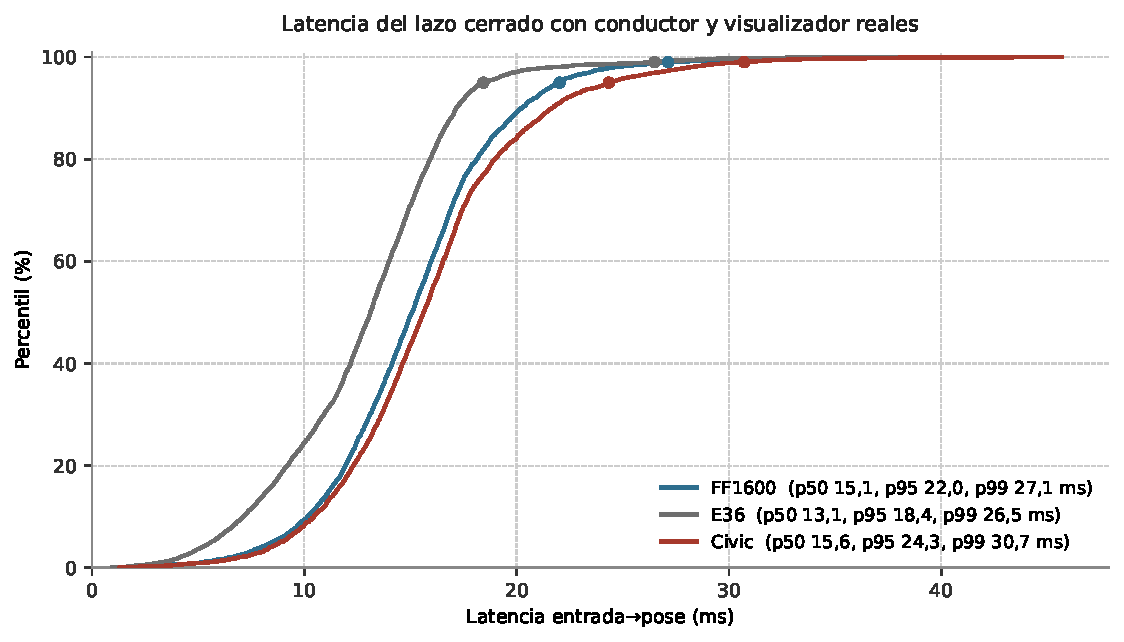
\includegraphics[width=0.86\textwidth]{img/latencia_lazo.pdf}
\caption[Distribución de la latencia del lazo cerrado]{Distribución acumulada de la latencia entrada$\rightarrow$pose para los tres vehículos. Los puntos marcan los percentiles $95$ y $99$. La mediana se sitúa entre $13$ y $16$ ms y la cola no supera los $31$ ms en el percentil $99$.}
\label{fig:latencialazo}
\end{figure}

\begin{figure}[H]
\centering
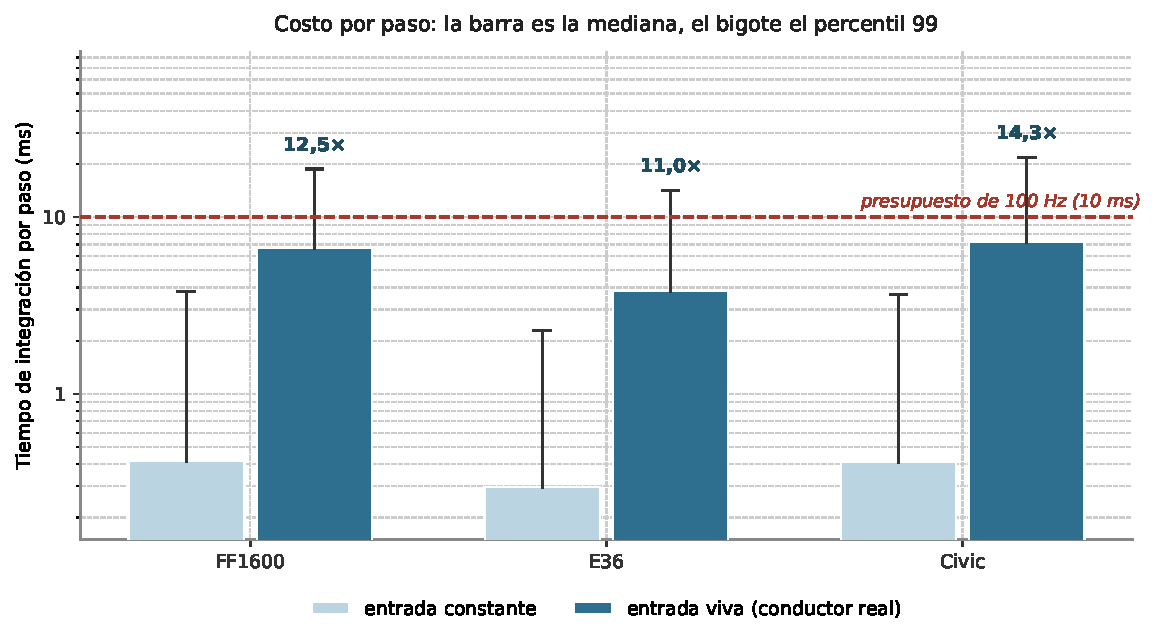
\includegraphics[width=0.86\textwidth]{img/paso_lazo.pdf}
\caption[Costo por paso con entrada viva y constante]{Tiempo de integración por paso en escala logarítmica. La barra es la mediana y la línea superior alcanza el percentil $99$. La línea discontinua marca el presupuesto de $10$ ms del paso de comunicación.}
\label{fig:pasolazo}
\end{figure}

Las nueve corridas completan su horizonte con un factor de $1{,}00\times$ respecto del reloj de tiempo real y sin descartar una sola pose. Se emitieron entre $22\,500$ y $22\,700$ datagramas por corrida, cinco por paso. La sincronización se mantiene con un período mediano de $10{,}07$ ms frente a los $10$ ms nominales.

Con medianas de $13$ a $16$ ms y percentiles $99$ de $26$ a $31$ ms, la contribución del modelo equivale a entre una y dos tramas a $60$ Hz. La antigüedad mediana del comando al aplicarse es de $7{,}6$ ms, mientras que la integración mediana cuesta entre $3{,}8$ y $7{,}2$ ms. Es decir aproximadente la mitad de la latencia no viene de la simulación si no de la espera del comando, sin embargo, siguen siendo valores bajos e imperceptibles para el humano.

Esta espera viene de la frecuencia de actualización del periférico. La separación mediana entre datagramas de comandos es de $15{,}60$ ms, equivalente a $64{,}1$ Hz, y no a los $100$ Hz que la aplicación de control asume. Elevar esta frecuencia reduciría el término dominante de la latencia. Un detalle a tener en cuenta es que la base utilizada en estas pruebas reporta una frecuencia de $1000$ Hz, por lo que esa limitante probablemente venga de la implementación de \textit{DeviceDrivers}.

Con la entrada constante, la integración cuesta entre $0{,}30$ y $0{,}42$ ms por paso, con el conductor real, entre $3{,}81$ y $7{,}24$ ms. El factor es de $11{,}0$ a $14{,}3$ según el vehículo. La causa de esto es la variación generada por la entrada: cada actualización del comando introduce un escalón en la señal mantenida, y con actualizaciones cada $15{,}6$ ms, prácticamente todo paso arrastra una perturbación que obliga al integrador a reducir el paso interno para recuperar la exactitud.

La consecuencia de esto es que las mediciones de lazo abierto obtenidas anteriormente, y particularmente los márgenes de $2{,}4\times$ a $16{,}1\times$ de la figura~\ref{fig:tiemporeal} son correctos para lo que miden, pero su comparación no es directa con la operación interactiva.


% \paragraph{La media no es la magnitud que importa.} Entre el $3{,}8\,\%$ y el $34{,}9\,\%$ de los pasos exceden el presupuesto de $10$ ms y, sin embargo, el lazo sostiene $1{,}00\times$ el tiempo real. La aparente contradicción se explica porque el acompasamiento solo espera cuando hay holgura: un paso de $16$ ms se compensa con los siguientes, que no duermen. En promedio el presupuesto se cumple; instante a instante, no. Contra la condición de control, donde apenas un paso de tres mil excede el presupuesto, queda claro que la ocupación pasa de un $4\,\%$ a un rango del $38$ al $72\,\%$ al cerrar el lazo con un conductor real. La holgura sigue existiendo, pero es un factor y no un orden de magnitud.

La extracción de las cinco poses y su conversión a cuaternión consumen entre $0{,}14$ y $0{,}20$ ms por paso, esto es, del $2$ al $3\%$ del total. La elección de Python para la aplicación de control no penaliza demasiado, la totalidad del costo reside en la integración, que ocurre en el código compilado de SUNDIALS.


\subsection{Limitaciones de esta medición} 
La conducción no fue guionada, los tres vehículos no se condujeron de forma idéntica, aunque se intentó mantener un comportamiento similar, por lo que las comparaciones entre ellos son indicativas y no controladas.


% \subsection*{Discusión}

% \paragraph{Robustez antes que velocidad.} El hallazgo más significativo de todo el capítulo no es de rendimiento sino de robustez, y los dos experimentos independientes coinciden en él. En el \textit{benchmark} de costo DASSL aborta en cuatro de seis configuraciones, incluida la totalidad de las que emplean terreno irregular; en la comparación de integradores aborta en dos de seis, y \verb|gbode| en una. CVODE, en cambio, completa las doce configuraciones de ambos experimentos sin una sola falla.

% Lo habitual al elegir un integrador es negociar entre velocidad y robustez. Aquí no hay tal negociación: CVODE es simultáneamente el más rápido —entre $1{,}5$ y $2{,}2$ veces más que DASSL, y entre $4$ y $6$ veces más que \verb|gbode|— y el único que nunca falla. La elección resulta, por lo tanto, inusualmente sencilla, y CVODE se adopta como integrador de referencia de la biblioteca.

% \paragraph{La tolerancia dejó de ser el factor limitante.} Los resultados de costo y de exactitud, leídos en conjunto, dan una respuesta clara al ajuste de la tolerancia. Del lado del costo, cada dos décadas de tolerancia adicional cuestan aproximadamente el doble de tiempo de cómputo. Del lado de la exactitud, esas mismas dos décadas reducen el error unos dos órdenes de magnitud. El intercambio es, por lo tanto, muy favorable a ajustar la tolerancia, y no existe razón de rendimiento para relajarla.

% Más relevante aún es la magnitud absoluta del error. Con la tolerancia $10^{-6}$ adoptada, la trayectoria se aparta de la de referencia entre $119$ y $233$ micrómetros al cabo de diez segundos de conducción, e incluso con la tolerancia más laxa ensayada el apartamiento máximo es de $2{,}1$ cm. Ambas cifras son varios órdenes de magnitud menores que la incertidumbre con la que se conocen los parámetros físicos del modelo —masas, rigideces, coeficientes de fricción, geometría de la suspensión—, que son en última instancia quienes acotan la fidelidad del simulador. El esfuerzo de mejora, por lo tanto, rinde mucho más aplicado a la caracterización del vehículo que al control de error del integrador.

% \paragraph{Las conmutaciones son la dificultad numérica dominante.} Un patrón atraviesa todos los experimentos de este capítulo: cada dificultad numérica observada se remonta a una no linealidad conmutativa, y ninguna al tamaño del sistema ni a la complejidad cinemática.

% La saturación del círculo de fricción degrada la convergencia de un factor $41$ a un factor $3{,}3$, hasta el punto de invalidar la maniobra agresiva como base de un estudio de exactitud. El modelo E36 multiplica por siete el número de muestras que devuelve al relajar la tolerancia, señal de un encadenamiento de eventos que no converge, y es el mismo modelo que aborta con $10^{-8}$ por exceso de iteraciones de evento y el único que ningún integrador alternativo consigue integrar. Las tres manifestaciones son caras distintas de un mismo problema. Y, en sentido inverso, las dos leyes de fuerza incorporadas al modelo físico —resistencia aerodinámica y resistencia a la rodadura— solo resultaron numéricamente inocuas porque se regularizó explícitamente su comportamiento en el entorno del reposo.

% La manifestación más costosa de todas, sin embargo, no está en el modelo sino en su entrada. El escalón que introduce cada actualización del comando del conductor multiplica por entre $11$ y $14$ el costo de integración respecto de una entrada constante, según se estableció en la sección anterior. Es la misma clase de perturbación —una discontinuidad que el integrador debe absorber reduciendo el paso— y su efecto supera a cualquier otro medido en este capítulo. Suavizar la reconstrucción del comando, en lugar de mantenerlo constante entre actualizaciones, es por lo tanto la optimización de mayor rendimiento potencial que este trabajo deja identificada.

% La lección práctica, transferible a modelos de esta clase, es que el esfuerzo invertido en suavizar de forma controlada las conmutaciones rinde más que el invertido en ajustar los parámetros del integrador. Una discontinuidad situada justamente en la condición de operación habitual —el reposo, en el caso de la resistencia a la rodadura— puede costar más que todo el resto del modelo.

% \paragraph{Costo del terreno irregular.} Para CVODE, pasar de terreno plano a sinusoidal multiplica el tiempo de simulación por factores de entre $1{,}9$ (FF1600) y $5{,}4$ (Civic). Esto es consistente con la naturaleza del modelo de contacto: sobre superficie plana la penetración del neumático se estabiliza en un valor cuasi-constante tras el asentamiento inicial, mientras que sobre el perfil sinusoidal oscila de forma continua, obligando al integrador a reducir el paso para seguir la dinámica vertical de la suspensión.

% \paragraph{Costo de inicialización.} La diferencia entre el tiempo total y el de simulación mide el costo fijo de inicialización y escritura de resultados. Para CVODE se sitúa entre $0{,}034$ y $0{,}090$ s, mientras que para DASSL alcanza aproximadamente $0{,}32$ s en las corridas completas. Aunque irrelevante para una simulación por lotes, este costo fijo sí importa en el arranque de una sesión interactiva.

% \paragraph{Complejidad del modelo y costo.} Confrontando los tiempos con la Tabla~\ref{tab:complejidad} se distinguen dos efectos separados. El primero sí responde al tamaño del modelo: el E36 tiene un $21{,}6\,\%$ menos de ecuaciones que los otros dos vehículos —consecuencia de que la suspensión \verb|McPherson|, construida sobre una única articulación \verb|Prismatic|, es cinemáticamente mucho más simple que el bucle cerrado del doble triángulo— y es, coherentemente, el más rápido sobre terreno plano: evaluar el lado derecho del sistema le cuesta menos.\\

% El segundo efecto no admite esa explicación. Los modelos \verb|Car| y \verb|CivicEKCar| tienen el mismo número de ecuaciones ($10\,981$), el mismo número de estados ($30$) y la misma topología de suspensión en las cuatro esquinas; sin embargo, sobre terreno sinusoidal el Civic tarda $2{,}85$ veces más que el FF1600. Con el tamaño del sistema fijo, esa diferencia solo puede provenir del número de pasos que el integrador necesita dar, es decir, de la rigidez numérica que introduce la parametrización concreta de cada vehículo: la masa suspendida, la rigidez del muelle y el amortiguamiento determinan la frecuencia propia del conjunto y, con ella, el paso máximo admisible. El Civic, con $990$ kg de masa suspendida sobre muelles de $16$ y $14$ kN/m, presenta una dinámica vertical más exigente de seguir que el monoplaza de $400$ kg.\\

% La conclusión práctica es que el costo de estos modelos tiene dos componentes independientes —el tamaño del sistema y la rigidez de la dinámica— y que reducir el primero, por ejemplo simplificando la cinemática de la suspensión, no reduce necesariamente el segundo.

% \paragraph{Qué limita realmente al simulador.} La exactitud no es la restricción: con errores del orden de las centésimas de milímetro y muy por debajo de la incertidumbre de los parámetros, el control de error del integrador no acota la calidad del resultado. El presupuesto de cómputo, en cambio, resulta bastante más ajustado de lo que las mediciones por lotes sugieren.

% La medición del lazo cerrado obliga a matizar los márgenes holgados de la Figura~\ref{fig:tiemporeal}. Al cerrar el lazo con un conductor real, la ocupación del presupuesto de $10$ ms pasa de un $4\,\%$ —con entrada constante— a un rango del $38$ al $72\,\%$, y entre el $4$ y el $35\,\%$ de los pasos individuales lo exceden. La holgura sigue siendo real, pero es un factor de dos o tres y no el orden de magnitud que el \textit{benchmark} por lotes anticipaba. Un modelo de neumático o de suspensión sensiblemente más detallado ya no entraría sin más.

% Las dos restricciones que gobiernan son, por lo tanto, la dispersión del tiempo por paso —no su media, dado que el acompasamiento compensa los excesos aislados a costa de la regularidad instantánea— y la robustez del modelo. El caso del E36 ilustra la segunda con claridad: un modelo puede resultar numéricamente frágil, hasta el punto de que dos de los tres integradores no logren integrarlo, con total independencia del margen de cómputo disponible. Y resulta llamativo que sea justamente el E36, el más frágil de los tres, el que menos cuesta en el lazo cerrado.

% Queda además una restricción que este trabajo no llegó a medir: la latencia total tal como la percibe el conductor. La contribución del modelo y su acoplamiento, de $13$ a $16$ ms de mediana, está caracterizada; la del periférico y la del renderizado en Unity, no.

% \subsection*{Limitaciones de la medición}

% Los tiempos del \textit{benchmark} de costo —Tablas~\ref{tab:tiempos} y \ref{tab:tolerancia}— corresponden a una única ejecución por configuración, sin repeticiones, por lo que no se dispone de una estimación de su dispersión. El estudio de exactitud sí repite cinco veces cada configuración, con desviaciones estándar de entre $0{,}01$ y $0{,}13$ s, lo que da una idea del orden de la variabilidad esperable también en aquellas mediciones. En una máquina de propósito general, con planificación de procesos y estados de caché variables, la variabilidad entre corridas idénticas puede ser significativa. Las conclusiones cualitativas —el orden de magnitud del margen respecto del tiempo real, y sobre todo el patrón de fallas de DASSL, que es determinista— son robustas frente a esa incertidumbre; las comparaciones finas entre vehículos, en cambio, deberían respaldarse con la media y la desviación estándar sobre un número suficiente de repeticiones.

% La medición del lazo cerrado, en cambio, sí informa percentiles sobre varios miles de pasos, y confirma la advertencia que motivaba esta precaución: un valor medio de tiempo por paso holgadamente inferior al umbral de tiempo real no garantiza por sí solo una experiencia interactiva satisfactoria, puesto que entre el $4$ y el $35\,\%$ de los pasos individuales exceden el presupuesto pese a que el promedio lo cumple. Su principal limitación es de otro tipo: la conducción no fue guionada, de modo que las comparaciones entre vehículos de esa sección no están controladas.

\section{Fidelidad del manejo}

Todas las mediciones anteriores son de carácter numérico, cuánto cuesta la simulación, cuánto tardan los integradores en coincidir, y con qué exactitud converge son medidas útiles para comparar el performance del modelo y de los integradores, pero no dicen nada sobre si el resultado se comporta como un vehículo real. Esta sección se centra en responder esa cuestión, comparando cuatro magnitudes del modelo contra lo que predice la teoría de dinámica vehicular y los valores típicos de automóviles reales.

Estos cuatro ensayos se eligieron por ser medibles sin instrumentar el modelo y cubren los ejes de la dinámica vehicular: el vertical, el lateral y el longitudinal.

\subsection{Frecuencia propia de la suspensión}

La frecuencia de la suspensión en su translación vertical (\textit{ride frequency}) es la manera más directa de medir el comportamiento vertical de un vehículo ante diferentes perturbaciones.

% La frecuencia de la suspensión en su modo de traslación vertical (\textit{ride frequency}) es el descriptor más inmediato del comportamiento vertical de un vehículo: fija la sensación de firmeza y determina el ancho de banda de las perturbaciones del terreno que la carrocería sigue.


% El ensayo se realiza, por lo tanto, dejando asentar el vehículo y perturbando después el estado correspondiente, con acceso al vector de estados a través de la interfaz de bajo nivel del FMU descrita en la Sección~\ref{sec:cosim}. Sobre la respuesta resultante se identifica un sistema de segundo orden, $\ddot{e} = -a\,\dot{e} - b\,e$, cuyo ajuste es lineal en los coeficientes y no depende de localizar máximos —escasos en una respuesta amortiguada—, de donde $\omega_n = \sqrt{b}$ y $\zeta = a / (2\omega_n)$.

Para realizar este ensayo se perturbó el estado de velocidad vertical del chasis, haciendo esto, los neumáticos conservan su compresión y los resortes de su deflexión al inicio, y al aplicar el impulso se excitan de forma natural, haciendo que el chasis se desplace mientras las ruedas permaneces quietas. El impulso empleado es de $0{,}05$ m/s, que produce amplitudes de $1{,}7$ a $2{,}4$ mm.

Sobre el resultado se obtiene un sistema de segundo orden. Dado que es un sistema resorte-amortiguador la ecuación que lo describe es la siguiente (escrita para un desplazamiento $e$ respecto a la altura de equilibrio).

\begin{equation}
    \ddot{e} = -\frac{c}{m}\,\dot{e} \;-\; \frac{k}{m}\,e
    \label{eq:segundo-orden}
\end{equation}

donde $m$ es la masa suspendida, $k$ la rigidez vertical y $c$ el amortiguamiento. De estos datos se pueden obtener la frecuencia natural y el amortiguamiento relativo:

\begin{equation}
    f_n = \frac{1}{2\pi}\sqrt{\frac{k}{m}},
    \qquad
    \zeta = \frac{c/m}{2\sqrt{k/m}}
    \label{eq:fn-zeta}
\end{equation}

El valor $R^2$ es el coeficiente de determinación, que es una medida de comparación entre el resultado esperado según la fórmula y el real, particularmente compara las aceleraciones. Un número cercano a 1 de de este valor confirmaría que este sistema es efectivamente de segundo orden y que no hay factores externos que lo modifiquen.

% El ajuste es lineal en ambos cocientes, de modo que tiene solución cerrada y aprovecha todas las muestras en lugar de depender de localizar máximos, que en una respuesta amortiguada son escasos. Su coeficiente de determinación $R^2$ sirve además de control: la Ecuación~\ref{eq:segundo-orden} es una hipótesis sobre el comportamiento del vehículo, no un hecho, y el $R^2$ mide si un único par de cocientes explica efectivamente toda la respuesta registrada. De no ser así, la frecuencia identificada no significaría nada.

% La Figura~\ref{fig:ajuste} superpone, para cada vehículo, la respuesta medida sobre el modelo y la función de segundo orden así identificada. La coincidencia es estrecha en el primer ciclo, que es donde reside la información sobre la frecuencia, y se abre en el rebote posterior: el modelo identificado predice un retroceso por debajo del cero algo mayor que el que el vehículo realmente describe. Esa discrepancia es la que explica que el $R^2$ se sitúe en torno a $0{,}97$ y no en la unidad, y su origen es que el vehículo completo no es un oscilador de un grado de libertad sino que acopla el modo vertical con el de cabeceo. El E36 es el caso que mejor ajusta, con $R^2 = 0{,}987$, y también aquel en que ambas curvas resultan casi indistinguibles.

\begin{figure}[H]
\centering
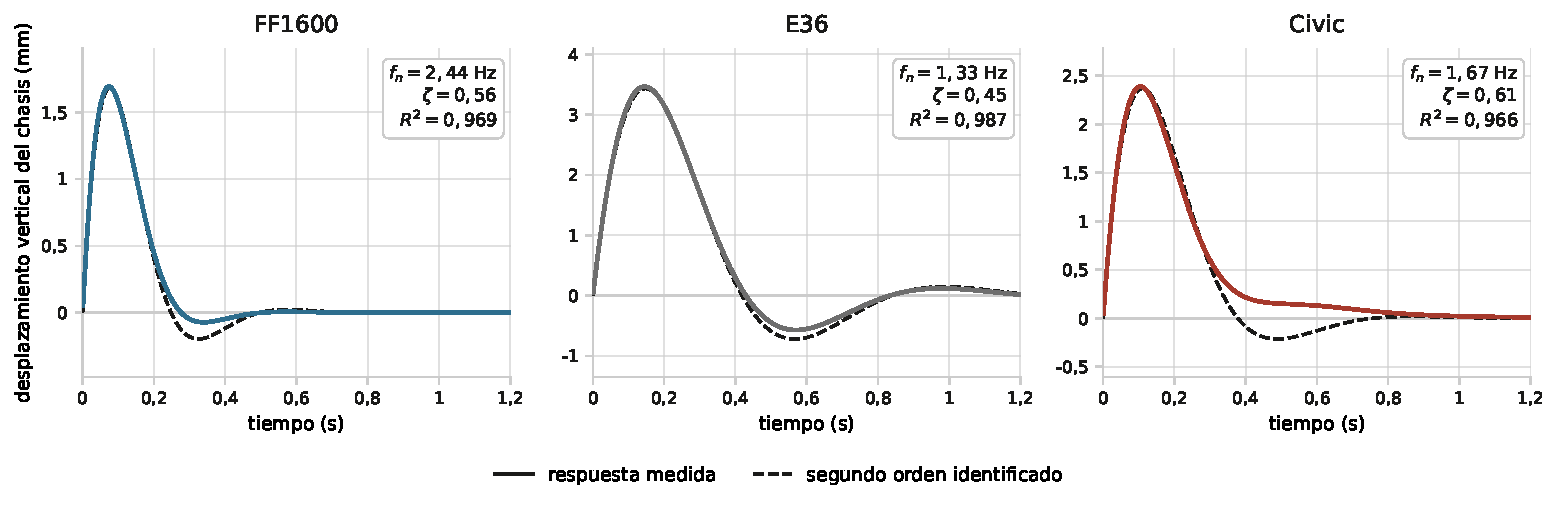
\includegraphics[width=\textwidth]{img/ajuste_segundo_orden.pdf}
\caption[Ajuste de segundo orden sobre la respuesta vertical]{Respuesta vertical libre del chasis tras el impulso de velocidad de $0{,}05$ m/s, en trazo continuo, y función de segundo orden identificada sobre ella, en trazo discontinuo. Un panel por vehículo, con las escalas verticales ajustadas a cada caso. Notar que las amplitudes son de apenas unos milímetros.}
\label{fig:ajuste}
\end{figure}

\begin{table}[H]
\centering
\begin{tabular}{lccccc}
\hline
Modelo & $f_n$ medida (Hz) & $\zeta$ & $R^2$ & Predicción (Hz) & Vehículo real (Hz) \\
\hline
FF1600 & $2{,}44$ & $0{,}56$ & $0{,}969$ & $2{,}42$ & $1{,}5$--$2{,}0$ \\
E36    & $1{,}33$ & $0{,}45$ & $0{,}987$ & $1{,}24$ & $0{,}5$--$1{,}5$ \\
Civic  & $1{,}67$ & $0{,}61$ & $0{,}966$ & $1{,}16$ & $0{,}5$--$1{,}5$ \\
\hline
\end{tabular}
\caption[Frecuencia propia y amortiguamiento de la suspensión]{Frecuencia natural y amortiguamiento relativo del modo vertical de la masa suspendida, identificados sobre la respuesta libre a un impulso de velocidad de $0{,}05$ m/s desde el estado asentado. La predicción es la Ecuación~\ref{eq:fn-zeta} evaluada con la rigidez y la masa declaradas en el modelo en lugar de con los cocientes ajustados, esto es $\frac{1}{2\pi}\sqrt{k_\text{ef}/m_\text{susp}}$, tomando el resorte en serie con la rigidez del neumático. La última columna muestra el rango habitual del tipo de vehículo que cada modelo representa. \cite{giaraffa_springs1}}
\label{tab:ride}
\end{table}

El caso del monoplaza da confianza en el procedimiento, su frecuencia medida coincide con la predicción teórica, es decir, para este vehículo el modelo se comporta como predice la fórmula. Los coeficientes de determinación confirman además que el modo es de segundo orden en los tres casos.

% \paragraph{El ensayo se valida a sí mismo.} El caso del monoplaza es el que da confianza en el procedimiento: su frecuencia medida, $2{,}44$ Hz, coincide con la predicción teórica, $2{,}42$ Hz, dentro del $1\,\%$. Es decir que para este vehículo el modelo se comporta exactamente como predice la fórmula elemental, lo que verifica a la vez la excitación empleada, el procedimiento de identificación y la propia predicción. Los coeficientes de determinación, entre $0{,}97$ y $0{,}99$, confirman además que el modo es efectivamente de segundo orden en los tres casos.

El resultado más interesante es la comparación con vehículos reales, para la que se toman como referencia los rangos de frecuencia de suspensión habituales en la práctica de la dinámica vehicular \cite{giaraffa_springs1,milliken1995}. El E36 se encuentra dentro de los rangos característicos de un vehículo de calle. En el caso del FF1600, si bien queda por encima del valor real esperado, este número no se pudo verificar con exactitud, principalmente por el hecho de que en autos de competición, los reglajes varían mucho entre equipos y circuitos, y no se tiene una fuente certera. Lo relevante, es que se ubica por encima de un vehículo de calle y por debajo de uno de competición con carga aerodinámica fuerte (entre  $3{,}0$ a $5{,}0$ Hz \cite{giaraffa_springs1}), por lo que es un punto medio en el que un monoplaza de este estilo puede vivir.


% El FF1600 queda donde corresponde un monoplaza sin carga aerodinámica, más duro que un vehículo de calle pero no tanto como un auto de competición con apoyo aerodinámico. En ambos casos el ensayo muestra que el comportamiento vertical coincide con el vehículo real.

El Civic también queda por encima del rango que le correspondería y es el que más se aparta de su predicción teórica. Esto se debe a que la predicción supone que el resorte se comprime lo mismo que la rueda, pero este está montado sobre los brazos de la suspensión, por lo que el cociente entre ambos recorridos (relación de instalación) depende de donde se fijen sus extremos. Calculando ese cociente en el modelo resulta en que el resorte recorre un $24\%$ más que la rueda, cuando en un vehículo real recorre menos de lo que recorre la rueda. Corregir los puntos de anclaje del conjunto resorte-amortiguador, llevándolos a una posición correspondiente al vehículo real ayudaría a que el modelo tenga valores más cercanos a la realidad, sin necesidad de tocar las rigideces declaradas.

% El Civic, con $1{,}67$ Hz, es el único que queda por encima del rango que le correspondería, y también el que más se aparta de su predicción teórica. Ambas desviaciones tienen la misma causa. La predicción supone que el resorte se comprime lo mismo que sube la rueda, pero el resorte no está montado sobre la rueda sino sobre los brazos de la suspensión, de modo que el cociente entre ambos recorridos —la \textit{relación de instalación}— depende de dónde se fijen sus extremos. En el Civic ese cociente vale $1{,}24$: el resorte recorre un $24\,\%$ más que la rueda, cuando en un automóvil real recorre \emph{menos}, entre un $50$ y un $70\,\%$ de lo que recorre la rueda. Como la rigidez percibida en la rueda escala con el cuadrado de esa relación, el vehículo resulta alrededor de un $50\,\%$ más rígido de lo que sus resortes declaran, y su frecuencia sube en consecuencia. Corregir los puntos de anclaje del conjunto muelle-amortiguador, llevándolos a una posición representativa de un vehículo real, situaría al Civic dentro del rango de calle sin necesidad de retocar las rigideces declaradas, que son valores realistas. Los otros dos vehículos no presentan el problema: el eje delantero del E36 tiene una relación de instalación de $1$ por construcción, su eje trasero de $0{,}92$ y el monoplaza de $0{,}97$.

El amortiguamiento relativo supera en los tres casos el rango habitual de $0{,}2$ a $0{,}4$ de un vehículo de calle \cite{giaraffa_springs3}, lo que se traduciría en una respuesta vertical algo más apagada que la real. Queda pendiente hacer una investigación más profunda para ver que puede llegar a causar esta diferencia.


\subsection{Cargas estáticas por rueda}

En equilibro, la velocidad vertical del contacto es nula, por lo que la ley de fuerza del suelo se reduce a $N = c \cdot (h + R_\text{wheel} - y)$ y la carga de cada rueda se obtiene de la altura de su centro, sin necesidad de exponer variables protegidas del modelo de contacto. La suma de las cuatro cargas debe igualar el peso total del vehículo, por lo que se va a realizar este ensayo para verificar la distribución de masas de el ensamblaje.


\begin{table}[H]
\centering
\begin{tabular}{lccccc}
\hline
Modelo & $N$ por rueda (N) & Total (N) & Masa implícita (kg) & Esperada (kg) & Reparto \\
\hline
FF1600 & $1343$ (las cuatro) & $5370$ & $547{,}4$ & $540$ & $50{,}0$ / $50{,}0$ \\
E36    & $2780$ / $2821$ & $11\,202$ & $1141{,}9$ & $1140$ & $49{,}6$ / $50{,}4$ \\
Civic  & $2789$ (las cuatro) & $11\,156$ & $1137{,}2$ & $1130$ & $50{,}0$ / $50{,}0$ \\
\hline
\end{tabular}
\caption[Cargas estáticas por rueda]{Cargas normales en equilibrio. En el E36 se indican las cargas delantera y trasera, que difieren; en los otros dos las cuatro coinciden. La masa esperada es la suma del chasis, los cuatro neumáticos de $20$ kg y los cuatro bujes de $15$ kg. El reparto es delantero/trasero en porcentaje.}
\label{tab:cargas}
\end{table}

El resultado tiene errores de entre el $0{,}6$ y el $1{,}4\%$, atribuible a la masa de componentes como brazos de suspensión, bujes, etc. que no se incluyen en la estimación. Esto valida la ley de contacto, la propagación del radio del neumático y el ensamblaje completo del vehículo. 

El reparto de cargas revela una limitación del modelo: los tres vehículos resultan equilibrados entre ejes, mientras que en la vida real esto no sucede siempre. Esto se debe a como está modelado el chasis, el hecho de que esté construido como un paralelepípedo de masa uniforme logra una abstracción que captura razonablemente las inercias pero no representa la posición longitudinal del centro de masa.

% El estado asentado muestra además una segunda limitación: la vía (distancia entre ruedas del mismo eje) es mayor de lo que debería en los tres vehículos. El E36 mide $2{,}02$ m de vía delantera y $1{,}96$ m trasera frente a los $1{,}42$ y $1{,}44$ m del vehículo real, el Civic $2{,}00$ m contra $1{,}47$ m y el FF1600 $2{,}46$ m. La causa es que no se pudieron obtener los valores del largo de brazos de suspensión el semiancho al que se fijan los anclajes ni la extensión lateral de los brazos se ajustaron a la geometría del vehículo que cada modelo representa. La consecuencia no es estética: una vía un $40\,\%$ mayor que la real aumenta en esa misma proporción el brazo de palanca con que las cargas verticales resisten el momento de vuelco, de modo que el modelo sobreestima la rigidez al balanceo y los límites laterales de la sección siguiente deben leerse como optimistas por ese motivo.



\subsection{Viraje y características laterales}

Para caracterizar el comportamiento lateral se realiza un ensayo de viraje con dirección constante. Se aprovecha el hecho de que con la resistencia aerodinámica incorporada cada valor de acelerador tiene su propia velocidad de equilibrio. El ensayo se realiza por valor de acelerador y se mide sobre los últimos cinco segundos, donde la velocidad casi no varía (menos del $6\%$ en todos los casos).

% Para caracterizar el comportamiento lateral se recurre al ensayo de viraje con dirección constante. Un ensayo a velocidad constante requeriría un regulador de velocidad, del que el modelo no dispone; en su lugar se aprovecha que, con la resistencia aerodinámica incorporada, cada valor de acelerador tiene su propia velocidad de equilibrio. Se realiza entonces un ensayo por valor de acelerador y se mide sobre los últimos cinco segundos, cuando la velocidad ya casi no varía —la deriva relativa en la ventana se mantiene por debajo del $6\,\%$ en todos los casos—, de modo que cada ensayo aporta un punto con el mismo ángulo de dirección.

\begin{figure}[H]
\centering
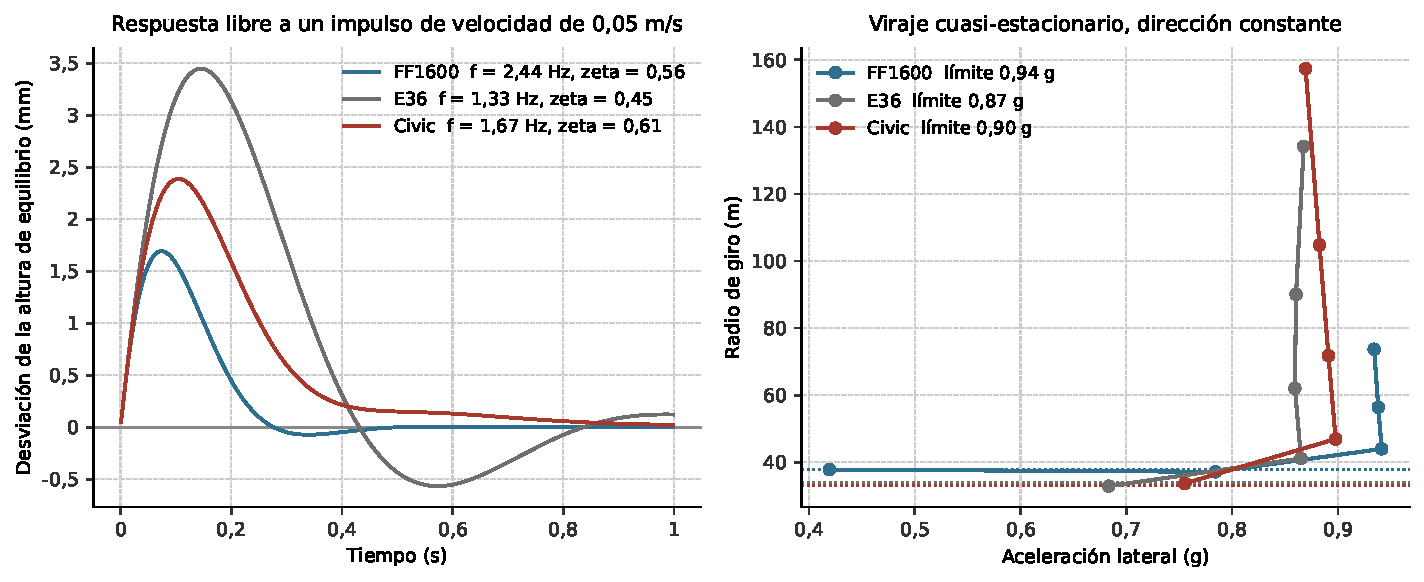
\includegraphics[width=\textwidth]{img/fidelidad.pdf}
\caption[Ensayos de fidelidad vertical y lateral]{Izquierda: respuesta libre del modo vertical tras perturbar en $5$ mm el estado asentado, con la frecuencia natural y el amortiguamiento identificados. Derecha: radio de giro en función de la aceleración lateral con dirección constante, un punto por valor de acelerador. Las líneas punteadas marcan el radio de Ackermann de cada vehículo, referencia de viraje neutro.}
\label{fig:fidelidad}
\end{figure}

La característica obtenida es la correcta, a baja aceleración lateral el radio se mantiene casi constante y a partir de cierto punto crece abruptamente sin que la aceleración lateral aumente, esto se debe a que el vehículo comienza a subvirar porque el neumático alcanzó su límite de adherencia.

% La característica obtenida es la correcta en su forma. A baja aceleración lateral el radio se mantiene aproximadamente constante y algo por encima del radio de Ackermann, y a partir de cierto punto crece abruptamente sin que la aceleración lateral siga aumentando: el neumático ha alcanzado su límite de adherencia y el vehículo se abre, esto es, subvira en el límite. Es el comportamiento que corresponde y el deseable desde el punto de vista de la seguridad.

El límite lateral alcanzado es de  $0{,}85$ g para el FF1600, $0{,}77$ g para el E36 y $0{,}85$ g para el Civic. Cabe aclarar que es un límite combinado y no puramente lateral, ya que al aplicar acelerador parte del presupuesto de agarre va también a la aceleración. Para un vehículo de calle sobre asfalto seco estos valores son válidos, sin embargo, para el monoplaza resultan bajos \cite{hyperphysics_tires}. Esto se debe a que el modelo de neumático utilizado fue el mismo para los tres vehículos, si se quisiera obtener un valor más preciso, habría que obtener y aplicar los parámetros de un neumático de competición.

% El ángulo de balanceo resulta remarcable. Los dos vehículos de calle se inclinan alrededor de $9$ grados por cada g de aceleración lateral (el E36 $6{,}8$ grados a $0{,}76$ g y el Civic $7{,}7$ a $0{,}82$ g) aproximadamente el doble de los $4$ a $5$ de un automóvil real. El monoplaza, con $3{,}3$ grados por g, queda donde corresponde.

% La causa es que no se implementó un modelo de barra estabilizadora, elemento del que un automóvil de calles obtiene buena parte de su resistencia al balanceo, lo que le permite montar resortes más blandos sin inclinarse demasiado al girar. El monoplaza no presenta esta falla debido a que un vehículo de competición si obtiene esa rigidez de resortes duros.  Agregarla es la corrección de fidelidad lateral más directa después de solucionar el reparto de pesos.


% El límite lateral alcanzado es de $0{,}74$ g para el FF1600, $0{,}70$ g para el E36 y $0{,}87$ g para el Civic. Conviene precisar que se trata de un límite combinado y no puramente lateral, puesto que el acelerador está aplicado y consume parte del presupuesto del círculo de fricción. Para un vehículo de calle sobre asfalto seco estos valores son verosímiles; para el monoplaza, en cambio, resultan bajos, ya que un vehículo de competición con neumáticos de compuesto blando supera holgadamente $1$ g.

% No fue posible extraer el gradiente de subviraje en el rango lineal. La resolución de acelerador disponible sitúa al vehículo por encima de $0{,}25$ g ya con el segundo valor ensayado, de modo que no se reúnen suficientes puntos por debajo del límite para ajustar una recta con sentido. Obtenerlo requeriría un regulador de velocidad que permitiera fijar pares (velocidad, radio) arbitrarios, lo que queda como trabajo pendiente.

\subsection{Distancia de frenado}

La prueba para verificar el comportamiento longitudinal consiste en acelerar y frenar a fondo luego de un tiempo determinado. Dado que este modelo no modela el downforce, la resistencia aerodinámica es menor, y tampoco tiene en cuenta la deformación del neumático, la frenada debe tener una desaceleración cercana al $1$ g, debido a que la carga normal del vehículo es solo su peso.

\begin{table}[H]
\centering
\begin{tabular}{lccccc}
\hline
Modelo & $v_0$ (km/h) & Distancia (m) & $a$ media (m/s$^2$) & $a$ media (g) & $a$ pico (m/s$^2$) \\
\hline
FF1600 & $93$  & $32{,}5$ & $10{,}18$ & $1{,}04$ & $10{,}92$ \\
E36    & $116$ & $51{,}4$ & $10{,}06$ & $1{,}03$ & $10{,}54$ \\
Civic  & $119$ & $54{,}6$ & $10{,}09$ & $1{,}03$ & $10{,}65$ \\
\hline
\end{tabular}
\caption[Distancia de frenado]{Frenada a fondo desde la velocidad indicada hasta la detención. La desaceleración media se calcula como $v_0^2 / 2d$.}
\label{tab:frenada}
\end{table}

Los resultados son consistentes con la cota mencionada anteriormente. Las desaceleraciones  medias del E36, Civic y FF1600 se sitúan justo sobre el límite de adherencia, superando el $1$ g debido al pico del inicio de la frenada. Las distancias resultantes coinciden con lo esperable.

% El monoplaza se detiene con una aceleración media menor, a pesa de que tiene el mismo coeficiente de fricción. Esto se debe a que la frenada no llega a alcanzar el agarre máximo de los neumáticos con el par que se le aplica, probablemente debido al menor peso del chasis. Si se quiere alcanzar una mejor frenada, se puede simplemente aumentar el parámetro de par máximo en el modelo para poder alcanzar el límite de adherencia.

Los valores pico superan la cota mencionada anteriormente porque corresponden a momentos transitorios en el momento de aplicar el freno, cuando la transferencia de pesos por el cabeceo del chasis incrementa la carga normal en el eje delantero, además de que la resistencia aerodinámica y de rodadura están más presentas a altas velocidades.



\subsection{Síntesis}

Tres de los cuatro ensayos dan resultados satisfactorios y el cuarto identifica una limitación concreta.

La contabilidad de las masas cierra con un error menor al $1{,}5\%$ con respecto a la suma de las masas declaradas, lo que valida la ley de contacto, la propagación del radio del neumático y el ensamblaje completo del vehículo. El comportamiento en frenada se corresponde a la cota del coeficiente de fricción y tiene valores coherentes con vehículos reales. El ensayo vertical sitúa tanto al E36 como al FF1600 dentro del rango esperado para la clase de vehículos que son.

La principal limitación es el reparto de cargas entre ejes, que es uniforme cuando no necesariamente debería serlo, esto es una consecuencia directa de modelar el chasis como un paralelepípedo con distribución de masa uniforme. Esta simplificación es la que más afecta al balance del vehículo y limita la fidelidad del comportamiento lateral. Una modificación en esta representación mejoraría la fidelidad significativamente.

% A esta limitación también se suma la ausencia de barras estabilizadoras: los dos vehículos de calle presentan un balanceo equivalente aproximadamente al doble del de un vehículo real. Agregar este componente es la segunda corrección en orden de importancia para mejorar la fidelidad, particularmente del viraje lateral.

% A ella se suma, en el mismo plano lateral, la ausencia de barra estabilizadora: con la vía en su valor correcto, los dos vehículos de calle acusan un gradiente de balanceo cercano a los $9$ grados por g, aproximadamente el doble del de un automóvil real, y en el límite su suspensión exterior alcanza los topes de compresión. Es la segunda corrección en orden de importancia, y no añade estados al sistema, ya que una barra estabilizadora es un resorte torsional entre las dos ruedas de un eje.

% A esto se suma una

% La limitación es el reparto de cargas entre ejes, uniforme cuando debería no serlo, consecuencia directa de modelar el chasis como un cuerpo de masa homogénea. Dado que ese reparto gobierna el balance del vehículo, es la simplificación que más acota la fidelidad lateral del modelo. A ella se suma, en el mismo plano lateral, una vía del orden de un $40\,\%$ mayor que la real en los tres vehículos, que sobreestima la rigidez al balanceo y obliga a leer los límites laterales medidos como optimistas. Son las dos magnitudes cuyo ajuste rendiría la mayor mejora de fidelidad, y ninguna de las dos exige cambios estructurales: la primera pide un chasis con centro de masa desplazado, la segunda un juego de anclajes y longitudes de brazo tomados del vehículo real.

Además quedan dos observaciones menos importantes: El Civic presenta una relación de instalación de $1{,}24$ cuando un automóvil real tiene alrededor de $0{,}5$ a $0{,}7$, lo que explica que la frecuencia vertical quede algo por fuera del rango de su tipo de vehículo. Revisar los puntos de anclaje del conjunto resorte-amortiguador, utilizando valores correspondientes a los reales debería corregir el problema sin modificar las rigideces declaradas. La otra observación es que en los tres modelos el amortiguamiento relativo excede el rango habitual.

Ninguna de estas limitaciones afecta a las conclusiones sobre desempeño de las secciones anteriores, pero si reducen la efectividad de su uso como simulador realista de conducción.

% Ninguna de estas limitaciones afecta a las conclusiones sobre desempeño de las secciones anteriores, que se refieren al costo y la exactitud de la integración y no al realismo del vehículo. Sí acotan, en cambio, el uso del simulador como herramienta de evaluación de comportamiento dinámico, y señalan con precisión qué habría que corregir para levantar esa restricción.

% Otra limitación, respecto al modelo de neumático, es que la fuerza lateral se modela como viscosa, proporcional a la velocidad lateral de deslizamiento, esto no tiene en cuenta, entre otras cosas la deformación del parche de contacto del neumático, ni el contacto de este en más de un punto del suelo. Esto se hizo para simplificar el sistema, debido a la complejidad que requiere desarrollar un modelo de neumáticos realista.

% Cabe añadir una limitación de fondo que estos ensayos ponen de manifiesto indirectamente. La fuerza lateral del neumático se modela como viscosa, proporcional a la velocidad lateral de deslizamiento, mientras que la de un neumático real es proporcional al ángulo de deriva, esto es, al cociente entre esa velocidad y la velocidad de avance. La consecuencia es que la rigidez de deriva efectiva del modelo crece de forma lineal con la velocidad en lugar de permanecer aproximadamente constante, lo que altera el balance del vehículo con la velocidad de un modo que no tiene contrapartida física. Sustituir la ley viscosa por un modelo basado en ángulo de deriva es, de todas las mejoras identificadas, la que más incidiría en la fidelidad del comportamiento lateral.


% Conclusions and Future Work
\chapter{Conclusiones y Trabajo Futuro}
\label{sec:conclusions}
El objetivo de esta tesina era desarrollar un simulador de dinámica vehicular capaz de ejecutarse en tiempo real con el conductor dentro del lazo. Las secciones que siguen resumen lo que el trabajo permite afirmar sobre ese objetivo, sobre las herramientas empleadas, sobre los límites que se encontraron y sobre mejoras posibles al proyecto.

\section{Conclusiones}

\subsection*{Es viable construir un simulador de conducción en Modelica}

La conclusión principal es positiva. Se pudo construir una biblioteca de dinámica vehicular multicuerpo en Modelica que acepta comandos de un conductor humano, o una herramienta externa, avanza la simulación al ritmo del tiempo real y devuelve la pose del vehículo a un entorno gráfico, todo con una latencia aceptable para la interacción con el ser humano. La mediana entre la recepción del comando y el envío de la pose es de entre $13{,}1$ y $15{,}6$ ms  y el percentil $99$ no supera los $31$ ms.



% El resultado no era evidente de antemano. Modelica es un lenguaje pensado para el modelado declarativo y la simulación por lotes, y su ecosistema no contempla la ejecución interactiva: no existe en él una noción de plazo ni de presupuesto de cómputo por paso, y el propio compilador asume que el integrador puede tomarse el tiempo que necesite. Llevar un modelo de esta clase a un lazo cerrado con un conductor exigió, por lo tanto, sacar el muestreo y el acompasamiento fuera del sistema de ecuaciones y dejar dentro únicamente la física continua. Esa separación, adoptada inicialmente para sortear una limitación de la herramienta, resultó ser la decisión de arquitectura más acertada del trabajo.

\subsection*{La composición orientada a objetos como herramienta de diseño}

Modelica organiza los modelos como componentes conectados por interfaces, esa estructura resultó determinante a la hora de implementar la biblioteca. Por ejemplo, las tres topologías de suspensión implementadas comparten una misma interfaz, por lo que cambiar la geometría de suspensión de un vehículo es tan simple como cambiar un bloque y sus parámetros con otro basado en esa misma clase. Esto se aplica a cualquier componente del vehículo, lo que permite la creación de diferentes variantes de manera muy simple.

Esto además permite la fácil expansión de la librería, por ejemplo, las barras estabilizadoras fue un componente que fue agregado a último momento, y lo único que se tuvo que hacer para implementarlo fue crear el modelo que lo represente y conectarlo a los marcos ya expuestos.
% Dos observaciones de este trabajo muestran que la propiedad no es solo declarativa. La primera es que los tres vehículos presentan exactamente el mismo número de estados continuos, treinta, pese a montar suspensiones de doble triángulo, de puntal telescópico y multibrazo: la interfaz común no impone un costo de representación, porque el cierre analítico del bucle cinemático evita introducir restricciones adicionales. La segunda es que incorporar la barra estabilizadora, un componente que no existía cuando se diseñaron las suspensiones, no requirió modificar ninguno de los modelos previos: bastó con escribir un componente nuevo que se conecta a los marcos ya expuestos.

% La parametrización también cumple un papel similar. Dos de tres vehículos representados tienen la misma geometría de suspensión, sin embargo son dos tipos de autos muy diferentes ( 

% La parametrización cumple el mismo papel a otra escala. Los tres vehículos representados —un monoplaza de escuela, una berlina de tracción trasera y un compacto de tracción delantera— se obtienen del mismo código cambiando masas, rigideces, radios y puntos de anclaje. Construir un cuarto vehículo no exige programar, sino medirlo.

\subsection*{El desacoplamiento por protocolo estándar}

La comunicación entre el simulador, el programa que controla el dispositivo de entrada y el entorno de visualización se resolvió utilizando UDP con un formato binario estandarizado. Esta elección de usar un protocolo de red en vez de, por ejemplo, una comunicación directa entre procesos, permite sustituir cada una de las piezas sin tocar las demás.

Los tres programas mencionados anteriormente son tres procesos independientes que solo comparten el mismo formato de mensajes. Durante el desarrollo se cambió la forma de ejecutar el modelo (de un ejecutable de OpenModelica a un FMU controlado desde Python) sin modificar ninguna línea del visualizador ni del programa de entrada. Esto permite en un futuro cosas como cambiar el visualizador por uno más avanzado, o distribuir los procesos en máquinas separadas.


\subsection*{El desempeño es holgado con CVODE}

A la hora de elegir integradores hay una clara elección, CVODE es a la vez el más rápido y el más robusto de todos los ensayados. Es entre $1{,}1$ y $1{,}3$ veces más rápido que CVODE, a la vez que más robusto en los casos de prueba y $3$ a $22$ veces más rápido que \verb|gbode|.

Con esa elección el márgen con respecto al tiempo real es más que suficiente. Ejecutando el modelo en lazo abierto está entre $2{,}4$ y $16{,}1$ veces con respecto al tiempo real. Al cerrar el lazo el márgen en menor, lo que es esperado debido a que la entrada deja de ser constante y el sistema debe coordinar la comunicación, pero sigue siendo suficiente, la latencia total se mantiene en el orden de la decena de milisegundos, lo que deja espacio para agregar modelos de suspensión o neumáticos más complejos por ejemplo.



\subsection*{Lo que limita la fidelidad no es el cómputo}

Los ensayos de fidelidad muestran que el techo del simulador no está en la parte numérica. Con la tolerancia elegida el apartamiento de la trayectoria respecto a una solución de referencia es de entre $47$ y $275$ micrómetros al cabo de diez segundos de conducción, incluso con la tolerancia más permisiva ensayada el error máximo es de $2{,}3$ cm. Son cifras con órdenes de magnitud menores que la incertidumbre con la que se conocen las masas, rigideces y geometría de las suspensiones.

Las limitaciones encontradas fueron de el último tipo mencionado. El reparto de cargas resulta uniforme porque el chasis se modela como un cuerpo de masa homogénea, lo que afecta a algunos modelos y la relación del conjunto resorte-amortiguador del Civic queda fuera del rango real porque no se tienen sus puntos de anclaje reales. Estos problemas se pueden solucionar agregando otra forma de modelar el chasis en el primer caso, y con datos en el segundo, en ambos casos es sencillo adaptar la solución al sistema ya existente.


% La conclusión práctica es directa. Disponer de medidas precisas de las dimensiones y de los puntos de anclaje de un vehículo real rendiría, en fidelidad, mucho más que cualquier refinamiento adicional del integrador o de la ley de contacto. El trabajo lo comprobó en sentido inverso más de una vez: corregir la ubicación de un anclaje cambió la frecuencia propia de una suspensión, su curva de caída y su vía, sin tocar una sola ecuación.

\subsection*{Las conmutaciones son la dificultad numérica dominante}

Un patrón que se repitió en todos los experimentos, y en particular en todos los obstáculos encontrados es que la principal dificultad numérica observada se debe a una no linealidad conmutativa y no al tamaño del sistema ni a una complejidad cinemática. Por ejemplo, los topes de suspensión son el origen de las fallas de integración más persistentes y el escalón que introduce cada actualización del comando del conductor multiplica el costo con respecto a una entrada constante.

Por lo tanto, es más rentable invertir esfuerzo en suavizar las conmutaciones que en intentar ajustar parámetros del integrador. Vale la pena prestar atención a las discontinuidades que se presentan cerca de la condición de operación habitual.

% La lección, transferible a modelos de esta clase, es que el esfuerzo invertido en suavizar de forma controlada las conmutaciones rinde más que el invertido en ajustar los parámetros del integrador. Conviene además prestar atención especial a las discontinuidades situadas en la condición de operación habitual: una regularización mal ubicada, justo donde el sistema pasa la mayor parte del tiempo, puede costar más que todo el resto del modelo.

\subsection*{OpenModelica como herramienta}

El balance sobre la herramienta tiene altos y bajos. Como entorno de modelado y de ejecución en lazo abierto, OpenModelica funcionó sin problemas, permite compilar los modelos multicuerpo con múltiples integradores, modificar sus parámetros de forma sencilla y expone herramientas de diagnóstico y visualización que permiten comprender como funciona el sistema.

% El balance sobre la herramienta es de dos caras. Como entorno de modelado y de ensayo en lazo abierto, OpenModelica cumplió sin reservas: compila modelos multicuerpo de varios miles de ecuaciones, ofrece tres integradores con los que contrastar resultados, expone las herramientas de diagnóstico necesarias para entender por qué un sistema es difícil de integrar, y permitió construir y validar la totalidad de la biblioteca.

Como entorno de ejecución en tiempo real mostró un problema que llevó a tener que buscar alternativas para este tipo de entorno: un reloj periódico de muestreo impide integrar con CVODE.

% Como entorno de ejecución en tiempo real, en cambio, mostró límites concretos. Se identificaron y documentaron cuatro defectos, cada uno con su caso mínimo de reproducción, y dos de ellos afectan de lleno al lazo cerrado: un reloj periódico de muestreo impide integrar con CVODE, y los FMU de co-simulación terminan durante el avance. El primero es el que obligó a trasladar el muestreo fuera del modelo; el segundo, a exportar como FMU de intercambio de modelos y proveer el integrador desde la aplicación externa.

Esta limitación no tiene que ver con el lenguaje Modelica, si no, viene de su implementación concreta del integrador CVODE específicamente. Aquí el carácter de software libre de OpenModelica permite la modificación de esta implementación, lo que hace que si se quisiese solucionar esta dificultad, se puede hacer sin problemas, en cambio una herramienta propietaria haría que se tenga que buscar una alternativa de forma obligatoria.

% Corresponde señalar que ninguna de esas limitaciones es del lenguaje Modelica, sino de una implementación concreta y de una versión concreta. Y aquí el carácter de software libre de OpenModelica deja de ser un detalle de licencia para convertirse en una propiedad técnica del proyecto: los cuatro defectos están documentados de forma reproducible, el código que los origina es público, y nada impide —a este trabajo o a otro— corregirlos en el propio compilador en lugar de rodearlos. Una herramienta cerrada con los mismos defectos habría dejado como único camino el que aquí se siguió, que es evitarlos.
\section{Trabajo futuro}

El simulador desarrollado es funcional y posee una arquitectura que permite su crecimiento sin rehacer lo construido. A continuación hay algunos puntos en los que el simulador se podría mejorar, las cuales podrían ser desarrolladas a partir de la base establecida en esta tesina.

% El simulador desarrollado es funcional y su arquitectura admite crecer en varias direcciones sin rehacer lo construido. Las líneas que siguen se ordenan de menor a mayor alcance: primero las que consisten en agregar componentes sobre las interfaces ya definidas, luego las que exigen revisar un modelo físico, y por último las que involucran al entorno de ejecución.

\subsection{Ampliación del catálogo de componentes}

La extensión más directa es agregar modelos nuevos sobre las interfaces definidas. Cada paquete de componentes de la biblioteca se define a partir de una clase base que fija su interfaz, por lo que un modelo nuevo se puede crear a partir de escribir la física correspondiente y adhiriéndose a la interfaz ya escrita, lo que permite que sea agregado a un vehículo sin modificar el resto de elementos.

Por ejemplo, un diferencial autoblocante sería una buena adición al sistema. El diferencial actual reparte el par por partes iguales en las dos ruedas, en cambio, un autoblocante transfiere par hacia la rueda con más agarre entre ambas salidas. Implementarlo simplemente consiste en crear un modelo a partir de la interfaz de diferencial y escribir la ley sobre los elementos de esta. De esta misma forma se pueden agregar geometrías de suspensión adicionales, frenos con distribución regulable entre ejes, entre otros.


\subsection{Modelo de transmisión y motor}

El tren motriz es actualmente la parte más simplificada del vehículo: el par motor se representa mediante un bloque que entrega un valor proporcional al input del acelerador, sin curva de par, relaciones de caja o embrague. Es suficiente para acelerar el vehículo y estudiar su comportamiento dinámico, pero se requeriría un modelo más complejo para simular correctamente un vehículo real.

El punto de conexión ya existe hoy en día, es la brida de par que alimenta al diferencial, por lo que agregar esto al sistema simplemente consiste en agregar el modelo y un input adicional de selección de marchas.

% La cadena de tracción es, hoy, la parte más simplificada del vehículo: el par motor se representa mediante un bloque que entrega un valor proporcional al comando del acelerador, sin curva de par en función del régimen, sin relaciones de caja y sin embrague. Es suficiente para acelerar el vehículo y estudiar su comportamiento dinámico, pero no para reproducir la conducción de un automóvil real, en la que el punto de cambio, la caída de par entre marchas y la respuesta del motor forman parte central de lo que el conductor percibe.

% Un modelo apropiado incluiría la curva de par en función del régimen, una caja con relaciones seleccionables, el embrague y la inercia rotacional de la cadena. La biblioteca \textit{Rotational} de Modelica provee los elementos necesarios, y el punto de conexión ya existe: es la brida de par que hoy alimenta el diferencial. Esta línea tiene además una consecuencia para el conductor humano, porque incorpora una entrada más —el cambio de marcha— al conjunto de comandos que el lazo ya transporta.

\subsection{Terreno con propiedades de superficie}

El modelo de contacto actual toma el coeficiente de fricción como un parámetro del vehículo, por lo que toda la pista tiene el mismo agarre. Darle propiedades locales al terreno leyendo el coeficiente de fricción en el punto de cada rueda, en vez de leerlo de un parámetro permitiría representar zonas de distinto agarre, superficies mojadas o pasto fuera de la pista, y lo haría sin alterar la estructura del modelo de contacto.

A esta mejora se lo podría sumar otra de consistencia. El terreno existe dos veces, una en el modelo físico y otra en el entorno gráfico, si se actualiza una, la otra también tiene que modificarse para que coincida. Unificarlas evitaría inconsistencias entre lo que ve el conductor y lo que se está calculando en la simulación, es particularmente útil en circuitos donde la geometría no es trivial.


\subsection{Modelo de neumático}

El neumático es un componente que mejorarlo aumentaría la fidelidad de forma significativa. La implementación actual es una simplificación de lo que se puede encontrar en una herramienta comercial, el desarrollo de un modelo de neumático realista podría ser una tesina por sí sola. Una mejora posible, por ejemplo, sería tener un modelo que habilite la elección de compuestos diferentes de neumáticos, esto permitiría poder diferenciar entre ruedas de calle o de competición, agregando fidelidad dependiendo del tipo de auto modelado.


% El neumático es el componente cuya mejora más incidiría en la fidelidad, por dos motivos distintos. El primero es de parametrización: un modelo que distinga compuestos permitiría diferenciar un neumático de calle de uno de competición, que hoy se representan variando un único coeficiente de fricción. El segundo es estructural y de mayor alcance: la fuerza lateral se modela como viscosa, proporcional a la velocidad lateral de deslizamiento, mientras que la de un neumático real es función del ángulo de deriva, esto es, del cociente entre esa velocidad y la de avance. La consecuencia es que la rigidez de deriva efectiva del modelo crece con la velocidad en lugar de mantenerse aproximadamente constante.

% Conviene señalar que un modelo de neumático más elaborado incorpora más no linealidades conmutativas, que es precisamente la clase de dificultad que este trabajo identificó como dominante: su implementación debería cuidar la regularización con el mismo criterio con que se cuidaron la resistencia a la rodadura y el círculo de fricción.

\subsection{Distribución longitudinal de masa}

El chasis se modela como un paralelepípedo de masa uniforme, por lo que el reparto de cargas entre ejes resulta simétrico. Es una limitación que en unos casos no es relevante (cuando el vehículo se acerca a esta distribución), pero en otros puede llegar a afectar significativamente a la fidelidad de la simulación, particularmente en su comportamiento lateral.

La corrección se podría hacer creando un nuevo modelo de chasis, que modele correctamente el desplazamiento del centro de masa, y en consecuencia, de una distribución entre ejes más realista. Para esto no es necesario hacer cambios estructurales, se puede lograr creando el modelo a partir de la interfaz ya definida. Se podría tratar de experimentar utilizando \verb|BodyShape| como reemplazo de \verb|BodyBox|.

% La corrección no exige cambios estructurales. Basta con desplazar el centro de masa del chasis respecto de su centro geométrico, o componer la carrocería a partir de varios cuerpos con masas y posiciones propias. Esta última variante tiene la ventaja de representar también las inercias con más realismo, y es la que mejor se presta a caracterizar un vehículo concreto a partir de datos reales.

\subsection{Retorno de fuerza al dispositivo de entrada}

El sistema de entrada actual es unidireccional, los comandos entran al simulador, pero el conductor no recibe feedback táctil de lo que esta sucediendo dentro del entorno. Agregar un retorno de fuerza agregaría esa funcionalidad y le daría al conductor información que ahora mismo solo se puede inferir de forma visual, como perdidas de agarre o cambios de elevación bruscos.

El sistema ya tiene lo necesario para hacerlo. Las fuerzan que tienen que enviarse ya se calculan dentro del modelo y el canal de comunicación no necesita grandes cambios, solamente hay que definir un mensaje más en el protocolo y reservar un puerto extra para eso.



% Esta línea vuelve exigible una medición que este trabajo no realizó: la latencia total del lazo tal como la percibe el conductor. Está caracterizada la contribución del modelo y de su acoplamiento, pero no la del periférico ni la del renderizado. Mientras el lazo es visual, un retardo adicional pasa relativamente inadvertido; con retorno de fuerza deja de hacerlo, porque el conductor lo percibe en las manos y la tolerancia es mucho menor.

\subsection{Suavizado de la reconstrucción del comando}

Entre las mejoras de rendimiento, una mejora potencial no está en el modelo si no en la entrada que le llega. Los comandos del conductor se reciben en intervalos discretos y se mantienen constantes entre actualizaciones, por lo que cada actualización genera un escalón que el integrador debe procesar, reduciendo el paso. Reconstruir el comando de forma continua (interpolando entre muestras por ejemplo) eliminaría estas discontinuidades sin alterar la física.

% Entre las mejoras de rendimiento, la de mayor efecto potencial no está en el modelo sino en su entrada. Los comandos del conductor llegan a intervalos discretos y se mantienen constantes entre actualizaciones, de modo que cada actualización introduce un escalón que el integrador debe absorber reduciendo el paso. Reconstruir el comando de forma continua —interpolando entre muestras, o filtrando la señal con una constante de tiempo pequeña frente a la respuesta del vehículo pero grande frente al paso de comunicación— eliminaría esas discontinuidades sin alterar la física.

% Es la aplicación directa de la lección que atraviesa todo el capítulo de experimentos, y la que mejor relación ofrece entre esfuerzo de implementación y margen de cómputo recuperado.

\subsection{Unificación del entorno de ejecución}

Toda la arquitectura de co-simulación adoptada existe porque OpenModelica no permite integrar con CVODE un modelo que tenga un reloj de muestreo. Corregir este defecto en el propio compilador permitiría ejecutar la totalidad del sistema desde OpenModelica, unificando todas las herramientas de la simulación en sí, lo cual es posible debido a la naturaleza de código abierto del compilador.



% La última línea no es sobre el simulador sino sobre la herramienta. La arquitectura de co-simulación adoptada, con el muestreo y el acompasamiento fuera del modelo, existe porque OpenModelica no admite integrar con CVODE un modelo que contenga un reloj periódico de muestreo. Corregir ese defecto en el propio compilador permitiría ejecutar el lazo cerrado íntegramente dentro de OpenModelica y disponer de una única herramienta para modelar, ensayar y ejecutar, en lugar de las dos que este trabajo debió combinar.

% El defecto está documentado en el apéndice con su caso mínimo de reproducción, que es el insumo que un informe al proyecto necesita. Vale aclarar que la corrección no invalidaría la arquitectura desarrollada: el desacoplamiento entre el motor físico, la entrada y la visualización seguiría siendo deseable por sí mismo, y de hecho es lo que permite sustituir el motor físico por otro. Lo que la corrección aportaría es la posibilidad de elegir, en lugar de la obligación de rodear una limitación.


\appendix
\label{sec:appendix}
\chapter{Defecto identificado en OpenModelica 1.25.5}
\label{sec:defectos}

En el desarrollo de esta tesina se identificó un defecto de OpenModelica~1.25.5 que condicionaron decisiones de arquitectura. Se documenta aquí con sus casos de reproducción para que puedan comunicarse al proyecto.

% En el curso de este trabajo se identificaron tres defectos de OpenModelica~1.25.5 que condicionaron decisiones de arquitectura. Se documentan aquí con sus casos mínimos de reproducción, tanto para justificar esas decisiones como para que puedan comunicarse al proyecto. Los tres se caracterizaron por eliminación, descartando una a una las causas alternativas.

\section{Un reloj periódico de muestreo impide integrar con CVODE}
\label{sec:defecto-reloj}



\paragraph{Síntoma.} Con el integrador CVODE, la simulación deja de avanzar en un punto de tiempo determinado (siempre constante con el mismo modelo) y emite indefinidamente el diagnóstico \textit{«Desired step to small»}. No hay mensaje de error ni terminación: la simulación queda consumiendo procesador sin avanzar.

\paragraph{Caso mínimo.} Basta con agregar a un modelo que funciona correctamente el siguiente fragmento:

\begin{verbatim}
discrete Integer ticks(start = 0, fixed = true);
equation
  when sample(0, 0.01) then
    ticks = pre(ticks) + 1;
  end when;
\end{verbatim}

La variable \verb|ticks| no está conectada a ningún componente y no interviene en otra ecuación. Con estar tres líneas el caso del modelo evaluado no supera nunca los  $19$ s, sin ellas completa $50$ s en $0{,}6$ s de cómputo. Tres bloques \verb|Modelica.Blocks.Discrete.Sampler| transmitiendo valores constantes producen el mismo efecto.

% La variable \verb|ticks| no está conectada a nada y no interviene en ninguna otra ecuación. Con estas tres líneas el modelo no supera los $19$ s; sin ellas completa $50$ s en $0{,}6$ s de cómputo. Tres bloques \verb|Modelica.Blocks.Discrete.Sampler| transmitiendo valores constantes producen el mismo efecto, al igual que una variante en la que el reloj alimenta un estado continuo aislado mediante \verb|der(x) = 1e-30*held|.



\paragraph{Descartado por medición.} El comportamiento es independiente de cualquier comando ingresado y del estado del vehículo, de la velocidad y distancia recorridas, de la vía de entrada de datos, del bloque\verb|RealtimeSynchronize|, de la representación de la orientación y de la frecuencia del reloj.



\paragraph{Alcance.} DASSL no presenta el problema, la consecuencia práctica es que CVODE resulta inutilizable para un sistema con intervención humana, que por definición muestrea su entrada. Es el defecto que motiva la arquitectura de la Sección~\ref{sec:cosim}.

% \section{\texttt{Frames.to\_Q} hace fallar al generador de código FMI}
% \label{sec:defecto-toq}

% \paragraph{Síntoma.} Un modelo que expone la orientación de un cuerpo como cuaternión, obtenido con \verb|Modelica.Mechanics.MultiBody.Frames.to_Q|, se exporta como FMU sin errores pero aborta al inicializarlo:

% \begin{verbatim}
% generic_array.c:72: check_copy_sanity:
%     Assertion `generic_array_ndims_eq(src, dst)' failed.
%     src->ndims != dst->ndims, 2 != 1
% \end{verbatim}

% El diagnóstico corresponde a la copia de una matriz de $3\times3$ sobre un vector de tres componentes en el código generado.

% \paragraph{Localización.} El mismo modelo se compila y simula sin dificultad como ejecutable autónomo, de modo que el defecto está en el generador de código FMI y no en el modelo. Se acotó comparando cuatro variantes que difieren únicamente en lo que exponen: una sin salidas, una con las tres coordenadas de posición y una con las nueve componentes de la matriz de rotación inicializan correctamente; la que expone el cuaternión mediante \verb|to_Q| es la única que aborta. La forma en que se declaran las salidas —arreglos o escalares— no influye.

% \paragraph{Alternativa.} Exportar la matriz de rotación y convertirla a cuaternión fuera del modelo.

% \section{Los FMU de co-simulación terminan durante el avance}
% \label{sec:defecto-cs}

% \paragraph{Síntoma.} Un FMU exportado con \verb|fmuType = "cs"| se instancia, supera la inicialización, configura el integrador —el registro muestra los parámetros de CVODE— y a continuación el proceso termina abruptamente, sin mensaje, dentro del primer segundo de tiempo simulado.

% \paragraph{Alcance.} Ocurre incluso con una envoltura que no expone ninguna salida, de modo que no depende de lo que el modelo comunique. Se verificó con los tres modelos de vehículo.

% \paragraph{Alternativa.} Exportar con \verb|fmuType = "me"|. El FMU de intercambio de modelos no contiene integrador propio, con lo cual el entorno de ejecución afectado no participa: la aplicación externa provee la integración. Con esta variante los mismos modelos completan sin dificultad horizontes de $50$ s.

% \section{Observaciones adicionales}

% Durante el trabajo se encontraron además tres comportamientos que, sin constituir defectos, resultan contraintuitivos y conviene registrar.

% \paragraph{\texttt{translateModelFMU} no genera archivo.} La instrucción traduce el modelo, informa éxito y no produce ningún FMU. La que genera el archivo es \verb|buildModelFMU|.

% \paragraph{Las opciones repetidas no se combinan.} Indicar dos veces \verb|-override| en la línea de órdenes produce el error \textit{«Command line option override is supposed to be combined on repetition. This has not been implemented yet»}; con \verb|-lv| la segunda aparición sustituye silenciosamente a la primera. Como OMEdit genera su propio \verb|-override|, los valores deben fijarse desde su interfaz y no agregarse a mano.

% \paragraph{\texttt{evaluateParameters} inhabilita las sustituciones.} Con el módulo de preoptimización \verb|evaluateParameters| activo, los parámetros se evalúan en tiempo de compilación y \verb|-override| deja de tener efecto sobre ellos, lo que impide barrer valores sin recompilar.


% just to avoid warning "Empty `thebibliography' environment". Remove after adding some citations
\nocite{*}

% Bibliography
\bibliographystyle{elsarticle-num}
\begin{small}
\bibliography{tesina}
\end{small}

\end{document}
